% *******************************************************************************
% ***               Edouard Leurent's "PhD Thesis" main file                    ***
% ***     Source code on: https://github.com/eleurent/phd-thesis/               ***
% ***     Original template: https://github.com/eleurent/phd-thesis-template     ***
% *******************************************************************************

% Class (remove "print" for digital version, remove "draft" for final version)
 \documentclass[a4paper,12pt,twoside,PageStyleII,custombib]{0-Misc/PhDThesisPSnPDF}
% \documentclass[a4paper,12pt,twoside,index,PageStyleII]{0-Misc/PhDThesisPSnPDF}
%\documentclass[a4paper,12pt,twoside,index,PageStyleII,print]{0-Misc/PhDThesisPSnPDF}

\title{Safe and Efficient Reinforcement Learning for Behavioural Planning in Autonomous Driving}
\author{Edouard Leurent}
\subject{This document is the PhD thesis of Edouard Leurent.}
\degreedate{October 2020}
\degreetitle{Thèse de Doctorat en Informatique}
\dept{Université des Sciences et des Technologies de Lille}
\college{Centre de Recherche en Informatique Signal et Automatique de Lille}
\university{École Doctorale Sciences pour l'Ingénieur}
\supervisor{Odalric-Ambrym Maillard \& Wilfrid Perruquetti}
\advisor{Denis Efimov \& Yann Blanco}
\keywords{%
	}

% FIXME compile with pdfx to have a PDF/A file
% \usepackage[a-1b]{pdfx}  % https://www.ctan.org/pkg/pdfx, PDF/A1-b for archiving

% --- Draft Mode
\SetDraftVersion{final}

% Packages (add your own packages here)
% --- French package
%\usepackage[french,greek]{babel}

% --- Front page Font
\newenvironment{frontfont}{\fontfamily{phv}\selectfont}{\par}
\DeclareTextFontCommand{\textFF}{\frontfont}

% --- Space between paragraphs/enums/items...
\setlength{\parskip}{0.5em}
\raggedbottom
\usepackage{etaremune}
\usepackage{enumitem}
\setlist[enumerate,itemize,description]{topsep=0em}

% --- Algorithms packages
\usepackage[algochapter,linesnumbered,commentsnumbered,inoutnumbered]{algorithm2e}

% --- Maths packages
\usepackage{amsmath}
% https://tex.stackexchange.com/a/12561/97964
\allowdisplaybreaks
\usepackage{amsthm}
\usepackage{amssymb}
\usepackage{bbm}
\usepackage{bm}
\usepackage{mathrsfs}
\usepackage{mathtools}
\usepackage{amsfonts}
\usepackage{empheq}
\usepackage{blkarray}

\usepackage{enumitem}
\usepackage{stmaryrd}

\usepackage{setspace}
\usepackage{stmaryrd}
\usepackage{cases}
\usepackage{stackengine}

% --- Figures and Captions
\usepackage{epstopdf}
\usepackage[small,bf,labelsep=endash,tableposition=bottom]{caption}
\usepackage{graphicx}
\DeclareGraphicsExtensions{.jpg,.pdf,.mps,.eps,.png}
% \usepackage{graphics}

% \usepackage{rotating}
% \usepackage{wrapfig}
\usepackage{float}
%\usepackage[caption=false,font=footnotesize]{subfig}
\usepackage[lofdepth,lotdepth]{subfig}
% \usepackage{subfigure}
% \usepackage{subcaption}
\newcommand{\subcaption}[1]{\caption{#1}}
\usepackage{cleveref}

% --- Figures Tikz
\usepackage{tikz}
\usetikzlibrary{positioning}
\usetikzlibrary{fit}
\usetikzlibrary{arrows}
\usetikzlibrary{shapes.geometric}
\usetikzlibrary{shapes.symbols}
\usetikzlibrary{backgrounds}
\usetikzlibrary{chains}
\usetikzlibrary{automata}
\usetikzlibrary{intersections}
\usetikzlibrary{decorations.pathreplacing}
\usepackage{tikzsymbols}  % http://texdoc.net/texmf-dist/doc/latex/comprehensive/symbols-a4.pdf for the \Coffeecup{} command!

% --- Color definition
\usepackage{xcolor}
\definecolor{Bleu}{RGB}{0,0,204}           % Define a new color rgb(0,0,204)
\definecolor{darkblue}{RGB}{0,0,126}       % Define a new color rgb(0,0,126)
\definecolor{Violet}{RGB}{102,0,204}       % Define a new color rgb(102,0,204)
\definecolor{deeppurple}{RGB}{102,0,204}   % Define a new color rgb(102,0,204)
\definecolor{darkgreen}{RGB}{0,100,0}      % Define a new color rgb(0,100,0)
\definecolor{lightgreen}{RGB}{185,220,87}      % Define a new color rgb(185,220,87)
\definecolor{gold}{RGB}{255,184,0}         % Define a new color rgb(255,184,0)
\definecolor{deepgold}{RGB}{205,105,0}     % Define a new color rgb(205,105,0)
\definecolor{Rouge}{RGB}{204,0,0}          % Define a new color rgb(204,0,0)
\definecolor{darkred}{RGB}{174,0,0}        % Define a new color rgb(174,0,0)
\definecolor{Highlight}{RGB}{251,0,0}      % Define a new color rgb(251,0,0)
\definecolor{gold}{RGB}{255,184,0}         % Define a new color rgb(255,184,0)

% --- Tables
\usepackage{booktabs}
\usepackage{multirow}
\usepackage{multicol}
\usepackage{rotating}
\usepackage{array}
\usepackage{multirow}  % https://en.wikibooks.org/wiki/LaTeX/Tables#Columns_spanning_multiple_rows
\usepackage{arydshln}
\usepackage{hhline}
\usepackage{makecell}
\usepackage[flushleft]{threeparttable}

% --- SI Units
\usepackage[binary-units,detect-all]{siunitx}

% --- Nomenclature
\usepackage{nomencl}
\makenomenclature

% --- Line Spacing
%\doublespacing
%\onehalfspacing
%\singlespacing

% --- Footnotes
%\usepackage[perpage]{footmisc}

% --- Bibliography
% Add `custombib' in the document class option to use this section
\ifuseCustomBib
	\usepackage[square,sort,authoryear]{natbib}
    %\usepackage[sort,numbers]{natbib}
	%\usepackage[backend=bibtex,style=alphabetic,natbib=true]{biblatex}
	%\renewbibmacro{in:}{}
	%\DefineBibliographyExtras{french}{\restorecommand\mkbibnamelast}
	%\bibliography{all-phd-thesis}
\fi

% changes the default name `Bibliography` -> `References'
\renewcommand{\bibname}{List of References}
\renewcommand{\contentsname}{Table of Contents}
\renewcommand{\nomname}{Abbreviations and Notations}

% --- User Defined
% \renewcommand{\partname}{Partie}
% \renewcommand{\chaptername}{Chapitre}
% \renewcommand{\listfigurename}{Liste des Figures}
% \renewcommand{\listtablename}{Liste des Tableaux}
% \renewcommand{\listlistingname}{Liste des Exemples de Programmes}
% \renewcommand{\appendixtocname}{Liste des Annexes}
% \renewcommand{\appendixname}{Annexe}

\newcommand*{\everymodeprime}{\ensuremath{\prime}}

% --- Table of Content
\setcounter{secnumdepth}{2}
\setcounter{tocdepth}{1}
% TODO FIXME change tocdepth to 1 for final version of the manuscript
\usepackage{minitoc}
\setcounter{minitocdepth}{1}

% --- Source code input, see https://en.wikibooks.org/wiki/LaTeX/Source_Code_Listings

\usepackage{framed}
%\usepackage[chapter,draft=false,final=true]{minted}

% https://tex.stackexchange.com/a/64845/97964
%\renewcommand{\listingscaption}{Code Example}% Listing -> Code Example
%\renewcommand{\listoflistingscaption}{List of Code Examples}% List of Listings -> List of Code Examples

% % https://tex.stackexchange.com/a/64845/97964
% \renewcommand{\lstlistingname}{Code example}% Listing -> Algorithm
% \renewcommand{\lstlistlistingname}{List of \lstlistingname s}% List of Listings -> List of Algorithms

% --- To Do notes
\ifsetDraft
	\usepackage[colorinlistoftodos]{todonotes}
	\newcommand{\TODO}[1]{\todo[inline]{TODO: #1}}
	\newcommand{\TODOE}[1]{\todo[inline,color=blue!40]{Edouard: #1}}
	\newcommand{\FIXME}[1]{\todo[inline]{FIXME: #1}}
\else
	\newcommand{\mynote}[1]{}
	\newcommand{\listoftodos}{}
	\newcommand{\TODO}[1]{}
	\newcommand{\TODOE}[1]{}
	\newcommand{\FIXME}[1]{}
\fi

%% Theorem English
%\newtheorem{theorem}{Théorème}[chapter]
%\newtheorem{lemma}{Lemme}[chapter]
% \newtheorem{proposition}{Proposition}[chapter]
\newtheorem{theorem}{Theorem}[chapter]
\newtheorem{assumption}[theorem]{Assumption}
\newtheorem{claim}[theorem]{Claim}
\newtheorem{corollary}[theorem]{Corollary}
\newtheorem{definition}[theorem]{Definition}
\newtheorem{defn}[theorem]{Definition}
\newtheorem{example}[theorem]{Example}
\newtheorem{lemma}[theorem]{Lemma}
\newtheorem{notation}[theorem]{Notation}
\newtheorem{proposition}[theorem]{Proposition}
\newtheorem{remark}[theorem]{Remark}

%\addto\captionsfrench{\def\figurename{{Figure}}}
%\addto\captionsfrench{\def\tablename{{Tableau}}}
%\addto\captionsfrench{\def\ALG@mname{{Tableau}}}
% \makeatletter
%\renewcommand{\ALG@name}{Algorithme}
% \makeatother
% \makeatletter
\newcommand{\clearevenpage}{%
	\clearpage%
	\if@twoside%
		\ifodd\c@page%
			\hbox{}\newpage%
			\if@twocolumn%
				\hbox{}\newpage%
			\fi%
		\fi%
	\fi%
}
\makeatother

\makeatletter
% https://tex.stackexchange.com/a/365249/97964
\def\cleardoublepage{%
	\clearpage%
	\if@twoside%
		\ifodd\c@page%
		\else%
			\hbox{}\thispagestyle{empty}\newpage%
			\if@twocolumn%
				\hbox{}\newpage%
			\fi%
		\fi%
	\fi%
}
% https://tex.stackexchange.com/a/365249/97964
\newcommand*{\cleartoleftpage}{%
	\clearpage%
	\if@twoside%
		\ifodd\c@page%
			\hbox{}\thispagestyle{empty}\newpage%
			\if@twocolumn%
				\hbox{}\newpage%
			\fi%
		\fi%
	\fi%
}
\makeatother

% https://tex.stackexchange.com/questions/25137/how-to-change-the-background-color-only-for-the-current-page
% \usepackage{afterpage}% for "\afterpage"
% \usepackage{pagecolor}% With option pagecolor={somecolor or none}
% \newcommand{\colorthispage}[1]{
% 	\newpagecolor{#1}%
% 	\afterpage{\restorepagecolor}%
% }
% \newcommand{\emptycolorpage}[1]{
% 	\newpagecolor{#1}%
% 	\newpage%
% 	\afterpage{\restorepagecolor}%
% }
% FIXME comment or uncomment if you need to compress the document
\newcommand{\emptycolorpage}[1]{
	% \null
	% \if@print
		% \clearpage%
		\cleardoublepage%
		% \cleartoleftpage%
		% \newpage%
		\thispagestyle{plain}%
		\null%
		% \pagecolor{#1}%  FIXME bring back color if I need
		\pagecolor{white}%
		% \null%
		\newpage%
		% \null%
		\pagecolor{white}%
	% \fi
}
% \newcommand{\emptycolorpage}[1]{\pagecolor{white}}

% Macros from Émilie Kaufmann's articles
\usepackage{0-Misc/macrosText}

% FIXME can I use the font I like?
% https://tex.stackexchange.com/questions/84770/using-palatino-and-euler-math#comment182397_84770
\usepackage{tgpagella}
% \usepackage{eulervm}


% pagecolorWhen  setting  the  background  color  with\pagecolor(a  commandfromcolor.sty), the first\pagecolormustprecede\usepackage{pdfpages}.\usepackage{color}\pagecolor{white}\usepackage{pdfpages}The color is nonrelevant, it can be changed afterwards by using\pagecoloragain.   Just  the  order  (first\pagecolorbefore\usepackage{pdfpages})  isimportant.
\pagecolor{white}
\usepackage{pdfpages}


% \usepackage{ifxetex,ifluatex}
% \ifnum 0\ifxetex 1\fi\ifluatex 1\fi=0% if pdftex
% 	\usepackage[T1]{fontenc}
% 	\usepackage[utf8]{inputenc}
% \else% if luatex or xelatex
% 	\ifxetex
% 		\usepackage{mathspec}
% 	\else
% 		\usepackage{fontspec}
% 	\fi
% 	\defaultfontfeatures{Ligatures=TeX,Scale=MatchLowercase}
% \fi
% % use upquote if available, for straight quotes in verbatim environments
% \IfFileExists{upquote.sty}{\usepackage{upquote}}{}
% % use microtype if available
% \IfFileExists{microtype.sty}{%
% \usepackage{microtype}
% \UseMicrotypeSet[protrusion]{basicmath} % disable protrusion for tt fonts
% }{}


\addbibresource{all-phd-thesis.bib}
\addbibresource{chapter*.bib}
\addbibresource{contributions.bib}

\begin{document}

	% ******************************** Preamble *********************************
	\frontmatter
	% List of included preambles goes here
%\begin{frontpage}
%\includepdf[pages={1}]{1-Preamble/1-Front/cover.pdf}
%\maketitle

%\end{frontpage}


\makeatletter
\def\parsecomma#1,#2\endparsecomma{\def\page@x{#1}\def\page@y{#2}}
\tikzdeclarecoordinatesystem{page}{
	\parsecomma#1\endparsecomma
	\pgfpointanchor{current page}{north east}
	% Save the upper right corner
	\pgf@xc=\pgf@x%
	\pgf@yc=\pgf@y%
	% save the lower left corner
	\pgfpointanchor{current page}{south west}
	\pgf@xb=\pgf@x%
	\pgf@yb=\pgf@y%
	% Transform to the correct placement
	\pgfmathparse{(\pgf@xc-\pgf@xb)/2.*\page@x+(\pgf@xc+\pgf@xb)/2.}
	\expandafter\pgf@x\expandafter=\pgfmathresult pt
	\pgfmathparse{(\pgf@yc-\pgf@yb)/2.*\page@y+(\pgf@yc+\pgf@yb)/2.}
	\expandafter\pgf@y\expandafter=\pgfmathresult pt
}
\makeatother

\begingroup
\thispagestyle{empty} % Suppress headers and footers on the title page


\begin{tikzpicture}[remember picture,overlay]
\node [rectangle, anchor=north, minimum width=\paperwidth, minimum height=\paperheight] (box) at (current page.north){};
%    \node[inner sep=0pt] (background) at (current page.center)
%    {\includegraphics[width=\paperwidth]{background2.pdf}};
\draw (page cs:0.,0.8) node [text opacity=1,inner sep=1cm]
{\large\centering\parbox[c][][t]{\paperwidth}
	{\centering Université des Sciences et des Technologies de Lille\\Ecole Doctorale Sciences Pour L'ingénieur}
};

\draw (page cs:0.,0.6) node [text opacity=1,inner sep=1cm]
{\large\centering\parbox[c][][t]{\paperwidth}
	{
		\centering {\LARGE\textsc{Thèse de Doctorat}}\\[0.8cm]
		\centering Spécialité \textbf{Informatique} \\[0.4cm]
		\normalsize présentée par\\
		{\Large \textbf{\textsc{Edouard Leurent}}}
    }
};

\draw (page cs:0.,0.35) node [inner sep=1cm]
{\large\centering\parbox[c][][t]{\paperwidth}
	{\centering  \par\noindent\rule{0.9\textwidth}{0.4pt}\\
		{\LARGE\textsc{Safe and Efficient Reinforcement Learning}\\ \textsc{for Behavioural Planning in Autonomous Driving}}\\
		 \par\noindent\rule{0.9\textwidth}{0.4pt}
}};

\draw (page cs:0.,0.1) node [text opacity=1,inner sep=1cm]
{\Huge\centering\parbox[c][][t]{\paperwidth}
	{\centering\normalsize sous la direction de \large \textbf{Odalric-Ambrym Maillard}\\
	\normalsize et de \large \textbf{Wilfrid Perruquetti},\\
	\normalsize ainsi que l'encadrement de \large \textbf{Denis Efimov}\\
	\normalsize et de \large \textbf{Yann Blanco}.}
};


\draw (page cs:0.,-0.15) node [text opacity=1,inner sep=1cm]
{
	\normalsize\centering
	\parbox[c][][t]{\paperwidth}
	{
		\centering \par\noindent\rule{0.5\textwidth}{0.4pt}\\
		Soutenue publiquement à \textbf{Villeneuve d'Ascq}, le \textbf{XX octobre 2020} devant le jury composé de
	}
};

\draw (page cs:0.,-0.35) node [text opacity=1,inner sep=1cm]
{\normalsize\centering\parbox[c][][t]{\paperwidth}
	{\centering
		\begin{tabular}{l l l}
		

		M. Lucian \textbf{Buşoniu} & Technical University of Cluj-Napoca & Rapporteur \\
		First Name \textbf{Last Name} & University & Rapporteur \\
		M. Marc \textbf{Deisenroth} & University College London & Examinateur \\
		First Name \textbf{Last Name} & University & Examinateur \\
		M. Odalric-Ambrym \textbf{Maillard} & Université de Lille & Directeur de thèse \\
		M. Denis \textbf{Efimov} & Université de Lille & Encadrant \\
%		M. Wilfrid \textbf{Perruquetti} & Centralle Lille & Directeur de thèse \\
%		M. Yann \textbf{Blanco} & Groupe Renault & Encadrant industriel
		\end{tabular}}
};

\draw (page cs:0.,-0.65) node [text opacity=1,inner sep=1cm]
{\normalsize\centering\parbox[c][][t]{\paperwidth}
	{\centering  \par\noindent\rule{0.5\textwidth}{0.4pt}\\
		Centre de Recherche en Informatique, Signal et Automatique de Lille (CRIStAL), \\UMR 9189 Équipe SequeL, 59650, Villeneuve d’Ascq, France}
};



\draw (page cs:0.,-0.8) node[inner sep=0pt]
{
	\hspace*{1em}
   	
\includegraphics[height=0.05\paperheight]{1-Preamble/1-Front/img/renault} \hspace*{1em}
   	
\includegraphics[height=0.05\paperheight]{1-Preamble/1-Front/img/univ-lille} \hspace*{1em}
   	
\includegraphics[height=0.05\paperheight]{1-Preamble/1-Front/img/CRIStAL} \hspace*{0.5em}
   	
\includegraphics[height=0.05\paperheight]{1-Preamble/1-Front/img/inria}
};

\end{tikzpicture}
\vfill
\endgroup

 % ******************************* Thesis Dedication ********************************

\begin{dedication}

    À mes grands-pères, Marc et Germain,\\ qui ont toujours nourri mon goût pour les sciences.

\end{dedication}
% FIXME declaration?
% % ******************************* Thesis Declaration ***************************

\begin{declaration}

% Author and date will be inserted automatically from thesis.tex \author \degreedate
Declaration of honor.

\end{declaration}


% FIXME bring back acknowledgement after sending/printing for reviewers
% ************************** Thesis Acknowledgements **************************

\begin{acknowledgements}
Un concept central en apprentissage par renforcement est celui du \emph{``credit assignment''} («~attribution du mérite~»). Selon ce principe, lors de l'obtention d'une haute récompense, il convient de remonter l'historique des évènements survenus par le passé afin d'identifier ceux qui furent responsables de ce succès.
Prêtons-nous à l'exercice.

Tout d'abord, je dois beaucoup à mes parents, ainsi qu'à mon frère et mes sœurs. Leur affection et encouragements constants au fil des années m'ont permis de m'engager avec confiance dans cette aventure.

Mais je n'aurais pas entrepris cette thèse sans l'exemple éclatant des doctorants de Parrot, Gauthier Rousseau et Clément Pinard, ni le concours de Jill-Jênn Vie, Edouard Oyallon, Alberto Bietti et Michal Valko qui ont tous conspiré à me mener au laboratoire SequeL. Je remercie également l'examen du permis de conduire, auquel mes échecs répétés m'ont permis de développer un intérêt égoïste mais pragmatique pour ce sujet de thèse en particulier.

J'adresse maintenant mes plus hautes \emph{traces d'éligibilité} ainsi que mes plus chaleureux remerciements à mes encadrants. Odalric et Denis, j'admire profondément votre intégrité et votre rigueur scientifique, ainsi que l'étendue de vos connaissances, que vous savez mobiliser pour répondre à la moindre de mes interrogations avec une facilité déconcertante. Merci également pour votre ouverture d'esprit, dont témoigne particulièrement la rencontre de vos disciplines respectives et la confrontation fructueuse des points de vue et des méthodes qui en découle. Mais avant tout, je vous suis reconnaissant pour votre bienveillance, votre disponibilité et votre soutien appuyé lorsque j'en avais besoin.
Yann, je te remercie pour avoir monté ce projet ambitieux, et pour m'avoir accordé une pleine liberté dans mes recherches, bien qu'elles se soient parfois écartées des préoccupations très concrètes de l'ingénierie Renault. Enfin, Wilfrid je te remercie pour tes précieux conseils toujours pertinents.

I am also very grateful to Lucian Busoniu and Jorge Villagra for their thoughtful reporting on this manuscript, as well as to all members of the jury, Luce Brotcorne, Marc Deisenroth and Rosane Ushirobira, for their valuable feedback, and for giving their time and energy to make it possible for my defence to take place amid the turmoil of a global pandemic despite being under lockdown.

J'en viens à mes coreligionnaires de la pause-café, avec qui j'ai pu décompresser, partager mes intérêts, mes joies et mes peines. A SequeL tout d'abord, je remercie particulièrement Mathieu et Xuedong, camarades de la première heure avec qui j'ai entamé d'inoubliables marches aléatoires dans les montagnes de Stellenbosch~; Nicolas et Omar, avec qui j'ai eu le privilège et le plaisir de collaborer~; Guillaume et Lilian dont l'éloignement rendait la visite occasionnelle d'autant plus festive~; Nathan et Dorian, dont l'appétence pour le débat n'a d'égale que leur propension à le trancher à coups d'étude ad-hoc~;  Pierre Ménard dont la cinéphilie et l'hospitalité ont permis la renaissance en grande pompe du Cinéquel~; Pierre Schegg, compagnon d'armes avec qui nous défendons fièrement le bastion des roboticiens à SequeL, ainsi que Florian, Ronan, Merwan, Mahsa, Julien, Yannis, Reda, Romain, Jean, Sarah et Antoine. Sans oublier les chercheurs~: merci Emilie, Jill-Jênn et Philippe pour vos contributions à la vie du laboratoire et à sa convivialité, ainsi que pour les collaborations et conversations scientifiques.
À Renault maintenant, Jean, j'ai su dès notre rencontre à Munich que ton goût communicatif et intarissable pour la philosophie nous conduirait à de précieuses et mémorables conversations. Merci également à Lu, Clara, Edwin, Federico, Louis et Thomas pour nos fameux repas-mini-doc\textsuperscript{\tiny\textsf{TM}}. Je salue aussi les doctorants du CAOR, Philip, Marin et Florent, avec qui il est toujours agréable de discuter, aux Mines ou en conférence, de nos approches différentes à un sujet commun.

Mais il y a une vie en dehors du travail, et je dois ses meilleurs moments à mes amis, merci Luc, Pierre, Bertrand, Adrien, Benjamin, Mano, Quentin, Thomas D., Thomas L., Simon, Oriane, Ivain, Magali et Daniel.

Enfin, merci Ariane pour ton soutien indéfectible, pour toutes tes qualités que j'admire tant, et pour me donner envie d'être et de donner le meilleur de moi-même.
\end{acknowledgements}
% ************************** Thesis Abstract *****************************
% Use `abstract' as an option in the document class to print only the titlepage and the abstract.
\begin{abstract}
% ----------------------------------------------------------------------------
\begin{center}
	\textbf{{\LARGE Résumé}}
\end{center}
% ----------------------------------------------------------------------------
\noindent
Dans cette thèse de doctorat, nous ...

% ----------------------------------------------------------------------------
\hr{}

% \newpage
% ----------------------------------------------------------------------------
\begin{center}
	\textbf{{\LARGE Abstract}}
\end{center}
In this PhD thesis, we...

\end{abstract}

%\begin{resume_fr}

% Résumé de la thèse en français.

% ----------------------------------------------------------------------------

%Ce manuscrit ...

% ----------------------------------------------------------------------------
%\section*{Contexte}
%
%\section*{Contributions}
%
%\section*{Organisation du manuscrit}


%% WARNING
%\vfill{}
%
%\hr{}
%
%\textbf{Note sur le droit intellectuel.}
%%
%Ce document est \href{https://github.com/eleurent/phd-thesis/}{publié} selon les termes de la
%\href{https://creativecommons.org/licenses/by-nc-sa/4.0/}{licence Creative Commons CC BY-NC-SA 4.0} (attribution - pas d'utilisation commerciale - partage dans les mêmes conditions),
%et les ressources additionnelles requises pour le générer (notamment les fichiers \LaTeX, les figures, etc.)
%sont \href{https://github.com/eleurent/phd-thesis/}{distribuées},
%sous la \emph{licence MIT} open-source,
%en ligne sur \href{https://github.com/eleurent/phd-thesis/}{\texttt{GitHub.com/eleurent/phd-thesis/}}.


%\begin{center}
%    \textbf{Copyright 2017-2020, \copyright ~Edouard~Leurent.}
%\end{center}


\end{resume_fr}



	% *************************** TOC ****************************
	\dominitoc
	\tableofcontents

	% *************************** Nomenclature ***************************
	%	\begin{spacing}{0.93}
	\glsaddallunused
	\printglossary[type=main, title={List of Acronyms}]
	\mtcfixglossary[chapter]
	
	\newcommand*{\Agroupname}{Mathematical notations}
	\newcommand*{\Bgroupname}{Markov Decision Processes}
	\newcommand*{\Egroupname}{Budgeted Reinforcement Learning}
	\newcommand*{\Zgroupname}{Linear Systems}
	\printglossary[type=symbols, title={List of Symbols}]
	\mtcfixglossary[chapter]
	%	\end{spacing}

	% *************** Chapters ****************
	\mainmatter

	%!TEX root = ../PhD_thesis__Edouard_Leurent
% Set counter to define 1st miniTOC.
\setcounter{mtc}{-1}
% FIXME change here if this issue happens again https://github.com/Naereen/phd-thesis/issues/4
\adjustmtc
% List of included chapters goes here

\part{First Part}
%!TEX root = ../../PhD_thesis__Edouard_Leurent.tex

\graphicspath{{2-Chapters/1-Chapter/}}

\chapter{Introduction}
\label{chapter:1}

\begin{flushright}
	\begin{tabular}{@{}l@{}}
%		\emph{What we call the beginning is often the end}\\
%		\hdashline
		\emph{We shall not cease from exploration}\\
		\emph{And the end of all our exploring}\\
		\emph{Will be to arrive where we started}\\
		\emph{And know the place for the first time.}\\
	\end{tabular}
	
	%T. S. Eliot, \href{https://eleurent.github.io/sisyphe/texts/little-gidding.html}{\enquote{Little Gidding}}. \emph{Four Quartets}.
	T. S. Eliot, \href{https://eleurent.github.io/sisyphe/texts/little-gidding.html}{\emph{Little Gidding}}.
\end{flushright}


\section{Context and scope}


\subsection{How should a driving robot make decisions?}
\label{sec:trolley}


\begin{figure}[tp]
	\centering
	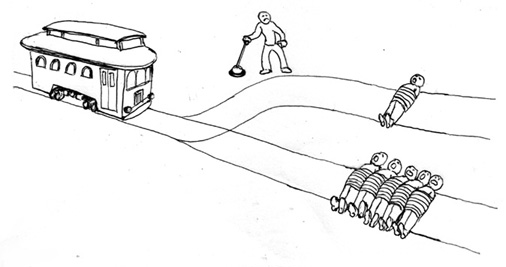
\includegraphics[width=0.7\linewidth]{img/trolley}
	\caption{The Trolley Problem \citep{Foot1967}. Illustration by \href{http://subcortex.com/}{Jesse J. Prinz}.}
	\label{fig:trolley}
\end{figure}

In the first few weeks of my Ph.D., I observed that layman interlocutors, when confronted with this question on the occasion of a social dinner, have a general tendency to conjure up disaster scenarios involving imminent accidents with unavoidable casualties. This reflex is likely to stem from the popularisation of the Trolley Problem \citep{Foot1967}, a famous thought experiment in moral philosophy, depicted in \Cref{fig:trolley}, in which a runaway trolley is headed straight toward five people tied up on the main track and unable to move. When pulled, a lever switches the trolley to a side track occupied by one person: what should you do? Answering this general question of what we \emph{ought} to do in any situation, what is a \emph{right} or \emph{wrong} decision, is the focus of the field of {normative ethics}. This dilemma illustrates a clash between two schools of thought: utilitarianism and deontological ethics. According to utilitarians, the rightfulness of an action should be evaluated based on its consequences, and actions maximising a \emph{utility} --the happiness and well-being for the affected individuals-- should be preferred. Conversely, deontologists evaluate the morality of actions \emph{per se}, according to a series of rules, rather than based on their consequences. Although this problem was initially introduced as a thought experiment, its transposition to the context of autonomous driving and arguably more realistic scenarios made it heavily cited in discussions regarding safety \citep[\eg][]{Lin2015,Bonnefon2016,Gogoll2017}. In early 2017, MIT's Media Lab launched the \emph{Moral Machine} platform \citep{Awad2018}, in which they invited members of the public to select the morally acceptable decision out of several options available to an autonomous vehicle. The authors argued that the recovered global preference would provide \emph{\enquote{essential topics to be considered by policymakers}}, and \citet{Noothigattu2018} proposed an implementation of a system aggregating these preferences, trained on the collected data. However, the relevance of this analogy to inform engineering and policy has been called into question. Thus, \citet{DeFreitas2019} point out that such dilemmas are unlikely to occur on real roads, hard to detect by perception systems and to act upon by control systems, and that they are distracting researchers from the more appropriate goal of how to avoid accidents altogether. Indeed, when we drive, we seldom find ourselves in such extreme situations but rather constantly ponder over less tragic considerations: Where does this vehicle intend to go? Do I have the time to proceed or should I yield? What is the appropriate speed to drive at right now? 
% https://www.grammarphobia.com/blog/2019/08/series-of-questions.html
The object of this thesis is to artificially reproduce this cognitive process of how to avoid accidents while driving, which is more a technical matter than an ethical one. Still, the Trolley Problem, though unrealistic, reveals and raises a number of legitimate questions. Should we base driving decisions on a set of rules? Can these rules be learned, \eg by imitating human drivers? Should we instead make decisions by comparing the utility of possible outcomes, like utilitarians advocate? And if so, how do we choose a good utility? This last interrogation becomes particularly sensitive if we add uncertainty to the Trolley Problem. Facing a potential collision, driving slowly decreases the risk of accident at the expense of efficiency, which can ultimately have an economical impact. What is the \emph{right} level of caution to take? This question directly translates as that of the \emph{value of life}, which has been taken up by economists for decades \citep{Abraham1960,Dreze1962,Schelling1968life,Banzhaf2014,Tirole2017,Charpentier2019} and has countless practical implications for public policies, including recent debates on lowering the speed limits on highways and trunk roads, but also on the appropriate lockdown durations during a pandemic.
It would be illusory to pretend that the practical implications of the Trolley Problem can simply be swept aside and entirely replaced by technicality. Throughout this manuscript, we will see that ethical concerns still underpin most assumptions and design choices of safety-critical software.


\subsection{Nuts and bolts of self-driving software}
\label{sec:nuts-and-bolts}

\begin{figure}[th]
	\centering
	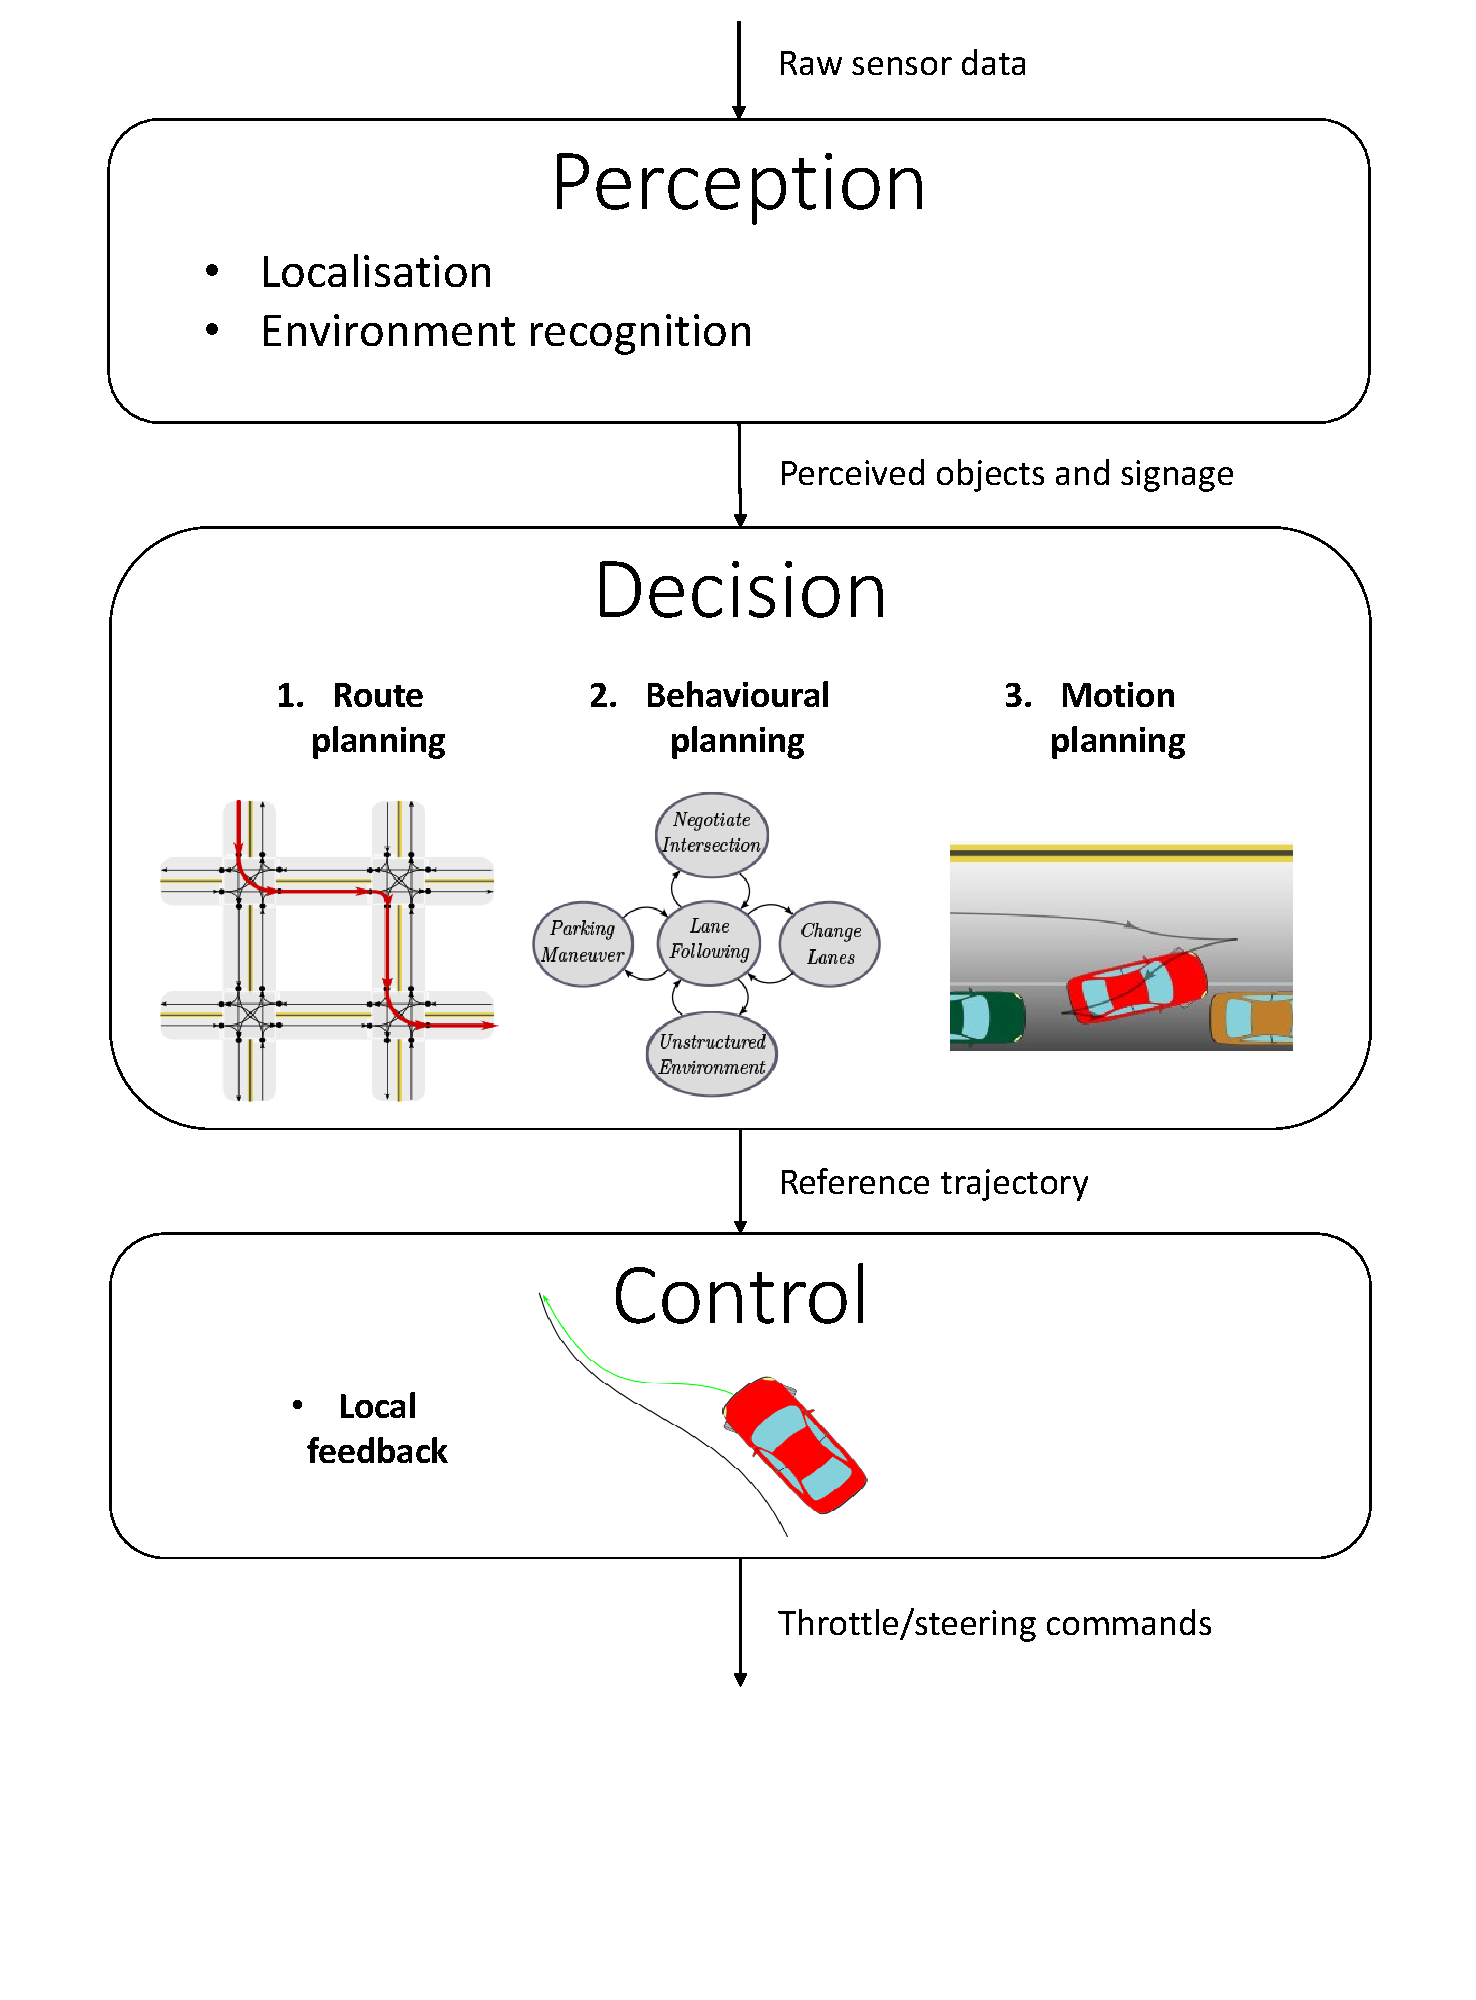
\includegraphics[trim={0 5cm 0 0}, clip, width=0.7\linewidth]{img/pipeline}
	\caption{The architecture of a typical self-driving software}
	\label{fig:robotics-pipeline}
\end{figure}

Historically, autonomous vehicles have been developed following a traditional robotics pipeline, illustrated in \Cref{fig:robotics-pipeline}. This architecture decomposes the task of driving as a series of three functions: \emph{Perception}, \emph{Decision}, and \emph{Control} (also called the Sense-Plan-Act paradigm, or Navigation, Guidance and Control in aerospace engineering). The {Perception} module takes raw sensor data as input and produces a high-level reconstruction of the scene. The {Decision} module then determines the desired trajectory of the vehicle, based on the current situation. Finally, the {Control} module manipulates forces, by way of steering and throttle controls, to track the desired trajectory. In the context of Autonomous Driving, the Decision module is often implemented with a hierarchical structure whose layers work at different timescales. First, a \emph{Route Planning} layer searches for the shortest route in a road network from the current location to the desired destination. Second, the \emph{Behavioural Planning} layer specifies a coarse driving behaviour through short-term goals or semantic decisions, such as changing lane, slowing down at an intersection, or yielding to a vehicle. This layer is thus responsible for following the planned route while adapting to the current state of the traffic in real-time. Third, the \emph{Motion Planning} layer generates a continuous, feasible trajectory that implements the desired behaviour while ensuring comfort and safety.

Great strides have been made in the two end-of-pipe tasks: Perception has benefited from the substantial progress in the field of computer vision due to the recent advent of deep learning \citep[surveyed in][]{janai2017computer}, and many Control schemes \citep[surveyed in][]{Polack2018} have been developed for ground vehicles. In the Decision module, Route Planning is virtually solved and already provided by services such as \href{https://wiki.openstreetmap.org/wiki/Routing}{Open Street Maps}, and there exist a vast body of Motion Planning algorithms, discussed in \Cref{chapter:2}. All these building blocks are widely used for industrial applications, including \gls{ADAS} functions such as \gls{LKA}, \gls{ACC}, \gls{AEB} or \gls{AES}; and in academic research challenges. Ultimately, we claim that Behavioural Planning remains the only neglected link in the chain. Indeed, most of these applications focused so far on simple settings with little complexity: \gls{ADAS} systems are mostly tailored for highway driving and struggle whenever required to interact with other drivers, \eg for merging into traffic\footnote{This difficulty, which motivated this thesis, was reported by engineers from the \gls{ADAS} team at Renault.}.
Similarly, most academic challenges focused on highway driving, with the exception of the DARPA Urban Challenge, which required more advanced interactions with other vehicles. Nevertheless, even this event still constituted a controlled environment, simple enough that all participants could rely on rule-based systems for behavioural planning \citep{Buehler2009}, such as finite state machines whose transitions are triggered by handcrafted criteria \citep[\eg][]{Baker2008}. Unfortunately, there is little hope that this approach can scale to complex scenes since responses tailored for specific use-cases cannot be easily merged. %TODO: ref needed

\subsection{Scope and Challenges of this Thesis}
\label{sec:scopes-and-challenges}

In the light of the above, this thesis is dedicated to addressing a weak link in the \gls{AD} chain: \emph{Behavioural Planning}.  We ask the following question: assuming that we had access to a ground truth perception and a perfectly accurate control system, what steps would remain to achieve fully autonomous driving?


\paragraph{Humans in the loop}

Unless restrained to dedicated infrastructure, Autonomous Vehicles will have to share the road with human drivers. This introduces a great deal of uncertainty in the decision problem. Indeed, while the location and velocity of a vehicle can be perceived, the mind of its driver remains impenetrable. Even though the present state is known, the future becomes uncertain: where are they headed? Are they paying attention to their surroundings? In that regard, it seems impossible to manually model all the factors involved in the human decision-making process. However, human drivers do not drive erratically either, and their behaviour is highly structured: humans drivers tend to follow the lanes, avoid collisions with other vehicles, and generally respect road signage. In other words, human drivers are \emph{predictable}. This motivates the idea of learning from data, and hope for a better comprehensiveness than handcrafted decision systems.%, either direct predictive models of human behaviours or a driving policy based on implicit predictions of what they might do next.
% We want to quantify uncertainty
% Recall aletoric vs epistemic uncertainty?

\paragraph{Learning to act}

The skill of driving a car involves taking a series of decisions, where early stages influence the resulting outcomes and subsequent reasoning at late stages. This aspect is known as sequential (or multistage) decision-making. Let us start by introducing some useful notations. At each time step $t$, the system is described by its \emph{state} $s_t$ that belongs to a measurable\footnote{A measurable space is a set with a $\sigma$-algebra, that allows to define random variables. For example, this set can finite ($[N]$), countable ($\Natural$), or continuous ($\Real$).} state space $\cS$. Then, the agent can take an \emph{action} $a_t$ within a measurable action space $\cA$, before transitioning to a next state $s_{t+1}\in\cS$, drawn from a conditional distribution $\Ps\parentheses{s_{t+1} \mid s_t, a_t}$ that we call the \emph{system dynamics} $\Ps\in\cM(\cS)^{\cS\times\cA}$, where $\cM(\cX)$ denotes the set of probability measures of a measurable set $\cX$. The agent actions can themselves be drawn from a distribution $\policy\parentheses{a_t\mid s_t}$, called the \emph{policy} $\policy\in\cM(\cA)^{\cS}$.

\gls{RL} is a general framework for learning-based sequential decision-making. It is formulated as an optimal control problem: the policy $\policy$ is chosen to maximise an objective function. It is generally formalised as a \gls{MDP}, \ie a tuple $(\gls+{cS}, \gls+{cA}, \gls+{transition}, \R, \discount)$ in which at each step $t$, the agent receives a bounded reward $R(s_t, a_t)$, where $R\in[0, 1]^{\cS\times\cA}$ is a deterministic reward function and $\discount\in[0,1)$ is a discount factor. Adequate long-term behaviour of policies $\policy$ is fostered by considering their \emph{return}.

\begin{definition}[Policy return]
	\begin{leftbar}[defnbar]
	The {return} $\return^{\gls+{policy}}$ of a policy $\policy$ is a random variable defined as the discounted sum of rewards 
	\begin{equation*}
	\gls+{return}^{\gls+{policy}} = \sum_{t=0}^\infty \discount^t \R(s_t, a_t)
	\end{equation*}
	accumulated along a trajectory $\tau = (s_0, a_0, s_1, a_1, \dots)$ induced by the policy $a_t\sim \policy(a_t|s_t)$ and system dynamics $s_{t+1}\sim \Ps(s_{t+1} \mid s_t, a_t)$.
	\end{leftbar}
\end{definition}

The performance of a policy $\policy$ is then evaluated through its \emph{value} function. 
\begin{definition}[Value functions]
	\begin{leftbar}[defnbar]
	\label{def:value-functions}
	The state value $\V^\policy(s)$ of a policy $\policy$ is the expected return of the policy when starting in a state $s$
	\begin{align*}
	\gls+{V}^\policy(s) \eqdef \expectedvalue\left[ \return^\policy \mid s_0=s\right].
	\end{align*}
	Similarly, the state-action value $\Q^\policy(s, a)$ of a policy $\policy$ is the expected return of the policy when starting in the state $s$ and taking the action $a$
	\begin{align*}
	\gls+{Q}^\policy(s, a) &\eqdef \expectedvalue\left[ \return^\policy \mid s_0=s, a_0 = a\right].
	\end{align*}
	\end{leftbar}
\end{definition}

This allows to define the goal of \glsxtrlong{RL}: finding an \emph{optimal} policy $\optimalpolicy$.

\begin{definition}[Optimality]
	\begin{leftbar}[defnbar]
	\label{def:optimality}
	A policy $\gls+{optimalpolicy}$ is said to be optimal if it maximises the value functions $V^\policy$ and $Q^\policy$ in every state and action.
	We also define the optimal value functions $\gls+{V}^\star$ and $\gls+{Q}^\star$ as 
	\begin{align*}
	&\forall s\in \cS, & \gls+{V}^\star(s) &\eqdef Q^{\policy^\star}(s) = \max_\policy V^\policy(s);\\
	&\forall (s,a)\in \cS\times\cA,& \gls+{Q}^\star(s, a) &\eqdef Q^{\policy^\star}(s, a) = \max_\policy Q^\policy(s, a).
	\end{align*}
	\end{leftbar}
\end{definition}

\paragraph{Sample efficiency}
Several performance measures have been introduced to evaluate \gls{RL} algorithms. In this thesis, we consider the goal of finding a near-optimal policy as fast as possible. The \emph{fixed-confidence} setting evaluates the smallest sample complexity, \ie number of interactions, required to find a near-optimal policy $\optimalpolicy$ with high probability. Alternatively, in the \emph{fixed-budget} setting, the \emph{simple regret} $\regret$ of an algorithm measures the \emph{expected} sub-optimality of the recommended policy $\hat{\policy}_n$ after a fixed number $n$ of interactions
\begin{equation*}
\gls+{regret}(s) \eqdef \expectedvalue_{\hat{\policy}_n} \left[ V^\star(s) - V^{\hat{\policy}_n}(s) \right].
\end{equation*}

%Conversely, in real environments where exploration is costly, another objective is to minimise the \textit{cumulative regret}.
%\begin{equation*}
%\cR_n(s_0, \cA) = \expectedvalue_{\hat{\policy}_t\sim \cA}\left[ \sum_{t=0}^{n-1} V^\star(s_t) - V^{\hat{\policy}_t}(s_t) \right]
%\end{equation*}

The goal of this thesis is to provide \emph{sample-efficient} algorithms for learning a driving policy. In the particular context of Behavioural Planning for Autonomous Driving, this goal will be articulated around a few main questions and challenges.

\paragraph{Model-free \vs model-based}

\glsxtrlong{RL} algorithms can be grouped into two main families. 
To find an optimal policy $\optimalpolicy$, model-based \glsxtrlong{RL} algorithms first attempt to estimate the \gls{MDP} parameters $\hat{P}$ and $\hat{R}$ based on a history of transitions $\cD = \{(s_{t},a_t, r_t, s_{t+1})\}$, using for instance \gls{MLE} in a hypothesis class of dynamics and reward functions:
\begin{equation*}
\max_{\hat{P}} \prod_{t}\hat{P}\parentheses{s_{t+1} \mid s_t,a_t} \quad \text{and} \quad \min_{\hat{R}} \sum_{t}\|R(s_t,a_t) - \hat{R}(s_t,a_t)\|^2_2.
\end{equation*}
This allows to \emph{plan} in the estimated \gls{MDP} $(\cS,\cA, \hat{P}, \hat{R}, \discount)$, \ie compute the associated optimal policy $\hat{\policy}^\star$. This can be achieved using planning algorithms such as Dynamic Programming or Linear Programming.
Conversely, model-free \gls{RL} algorithms do not estimate the underlying \gls{MDP} and aim instead to optimise a policy $\policy$ directly. Policy-based methods evaluate the value $Q^\policy$ of the current policy $\policy$, so that it can be locally improved \eg by gradient ascent. Value-based method bypass this alternation of evaluation and improvement steps by directly learning the optimal value function $Q^\star$.

The question of which approach is appropriate depends on the underlying problem. Indeed, model-based techniques are relevant when the dynamics are simple but the optimal policy is complex. For instance, the case of Computer Go was tackled in AlphaGo \citep{Silver2016,Silver2017,Silver2018} with a \gls{MCTS} planning module, which leveraged the knowledge of the Go dynamics (placing pawns on the board) to sample sequences of plies in a game tree. On the contrary, the model-free approach is useful when the system dynamics are complex, but the optimal policy is simple. Thus, a swimming robot would require massive fluid dynamics simulation to accurately predict the effect of moving its fins, while a simple periodic gait could suffice to propel it forward in the water. Which brings us to the question: which scenario does \gls{AD} fall into? Unfortunately, the answer is not so clear-cut. On the one hand, the motion planning literature has historically been heavily relying on kinematics and dynamics models to plan trajectories, as detailed in \Cref{chapter:2}. Reliable priors are available to describe the physics of a vehicle, but not so much for the actual driving policy. On the other hand, automotive companies such as Mobileye reportedly\footnote{These comments are reported from discussions between Renault and Mobileye.} advocated that the task of predicting a driving scene is actually more difficult than that of driving. In fact, the case of \glsxtrlong{AD} is peculiar in that the two problems of prediction and control are somewhat equivalent, due to the presence of other drivers: a good trajectory predictor can be used to predict the action that a human would take in place of the ego-vehicle, and a good driving policy can be applied to each agent in the scene to produce reasonable predictions of their trajectory. Hence, both approaches seem equally relevant and will be considered in this thesis.

\paragraph{Social interactions and coupled dynamics}

To ensure safety while driving, traditional motion planning techniques rely on conservative independence assumptions on the behaviour of other vehicles. This makes them suffer from an effect colloquially known as the \emph{\enquote{freezing robot problem}} \citep{Trautman2010}: due to massive uncertainty, these systems tend to struggle in situations that require interacting --or negotiating-- with other vehicles, such as unprotected left-turns, intersections, or highway merges (see \eg these \href{https://www.youtube.com/watch?v=HjtiiGCe1pE}{two} \href{https://twitter.com/nitguptaa/status/990683818825736192}{videos} where a Waymo car fails to merge). 
Thus, for an autonomous vehicle to efficiently integrate with the traffic flow, it must anticipate the effect of its own actions on the behaviour of other agents. This skill is known as \emph{socially-aware} decision-making. Unfortunately, interactions between vehicles translate into complex and coupled traffic dynamics where local deviations must be propagated from one vehicle to the next, which can result in a quick and chaotic build-up of uncertainty. We will need to contain this escalation to prevent instability in our predictions.

\paragraph{Ensuring safety}

The complexity of the task of driving leads us to consider learning algorithms. However, these methods typically raise a legitimate concern among car manufacturers: how can we guarantee the \emph{safety} of such systems, in the presence of uncertainty? In this thesis, we will strive to formalise this concern by formulating different notions of \emph{risk}, as functions of the distribution of outcomes induced by a policy. We will study \emph{Safe} \glsxtrlong{RL} algorithms, that seek to explicitly estimate and control the level of risk taken by a policy.

\paragraph{Balancing safety and efficiency}
However, protecting against risk often comes at the price of efficiency in achieving a goal.
Consider for a moment a situation where a vehicle is driving slowly in front of you on the road, and so you decide to overtake them. How do you know, at that very moment, that the driver has seen you and is not going to change lane at the last moment, causing an accident? In fact, you don't, at least not with certainty. In this situation, the only way to guarantee safety is to refrain from overtaking. By pushing this simple argument through to its conclusion, it becomes apparent that the only way to \emph{fully} ensure safety is to stay in the garage.
You are thus facing an irreducible dilemma: the two objectives of driving fast and safely are contradictory.
This opposition induces a trade-off that we typically observe with human drivers, especially in situations of negotiations: some people adopt \emph{aggressive} behaviours and try to force their way through traffic, while others act more \emph{defensively}, favouring safety. This ambiguity is difficult to capture manually in an objective function and soon leads to the pitfall of reward engineering. To provide a principled control over this trade-off, the learning algorithms that we consider will be required to respect an \emph{adjustable} level of risk.

\section{Outline and Contributions}

\begin{figure}[ht]
	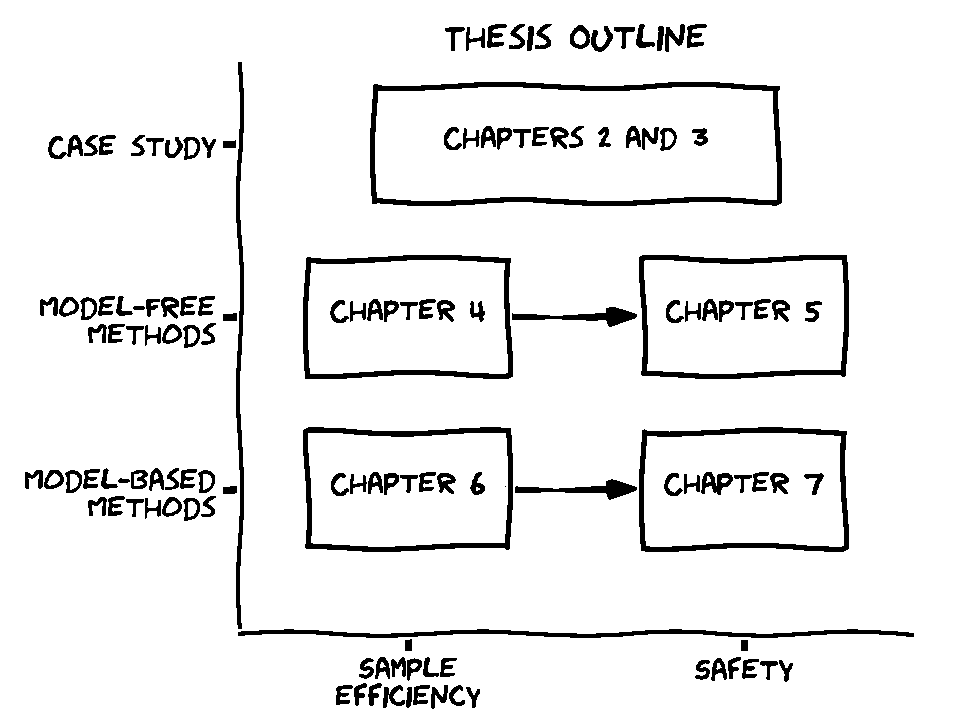
\includegraphics[width=0.9\linewidth]{img/outline}
	\caption{This thesis is structured around two disjunctions: model-free \vs model-based on the one hand, and sample-efficiency \vs safety on the other hand.}
	\label{fig:thesis-outline}
\end{figure}

% Part I
The ultimate goal of this thesis could be summarised in the following question: \emph{\enquote{how can an algorithm learn to drive and avoid accidents?}}. The first step in such an endeavour must necessarily be to formalise more precisely the meaning of this ill-posed formula, which we try to do in \textbf{\Cref{part:1}}.
It is only natural that we begin this effort by turning to the standard model for sequential decision making: the \glsxtrlong{MDP}. At first glance, this framework shines with its simplicity and elegance, but also its apparent generality and representation power. Yet, as we embark on the ambitious task of casting the blurry problem of autonomous driving into this rigid mould, we highlight in \textbf{\Cref{chapter:2}} how reductive each step of the formalisation is, how approximations and assumptions always hide behind each symbol and each equation. This observation is supported by the numerous variations of the framework developed by the research community, in as many attempts to address these concerns. Such limitations are as varied as partial observability, temporal abstraction, the reward hypothesis, transfer from simulation to real-world and safety; and we relate these research directions to specific works in the autonomous driving literature.

In order to progress, we put aside some of these questions in \textbf{\Cref{chapter:3}} and commit to an (observable) state space, a (hierarchical) action space, a (quasi-linear) system dynamics and a (dense) reward function that we deem suitable for a large class of behavioural planning tasks. This allows us to refocus on two fundamental issues: \textit{sample-efficient} and \textit{safe} \glsxtrlong{RL}. In the sequel we tackle them through the perspective of the two main approaches to \glsxtrlong{RL} aforementioned: first model-free, and then model-based algorithms. This organisation is depicted in \Cref{fig:thesis-outline}.

% Part II
\textbf{\Cref{part:2}} is dedicated to the study of how model-free methods can be applied for efficient and safe \glsxtrlong{AD}. In \textbf{\Cref{chapter:4}}, we question the choice of state representation and model architecture in relation to their associated sample-efficiency. In particular, we identify desirable properties and inductive biases that the policy should enjoy, such as \emph{permutation invariance} with respect to vehicles in the scene. We propose an attention-based architecture that fulfils our criteria, and compare it to standard representations and model architectures that have been used for behavioural planning tasks. 

In \textbf{\Cref{chapter:5}}, we consider a continuous notion of risk, defined as an expected discounted sum of a cost signal. This formulation allows highlighting  a trade-off between two separate objectives: the traditional return associated with task completion, and the risk related to safety. In this multi-objective perspective, the Pareto frontier of non-dominated policies defines a spectrum of behaviours, from risk-averse on one side to risk-seeking on the other. In order to explicitly control the level of risk taken in real-time, we place ourselves within the \gls{BMDP} framework, in which the risk is constrained to lie below an --adjustable-- threshold. 
So far, \glspl{BMDP} could only be solved in the case of finite state spaces with known dynamics. This chapter extends the state-of-the-art to environments with continuous state space and unknown dynamics. We show that the solution to a \gls{BMDP} is a fixed point of a novel Budgeted Bellman Optimality operator, which enables to estimate both the expected return and risk of an action, in a model-free fashion. This observation allows us to introduce natural extensions of Deep Reinforcement Learning algorithms to address large-scale \glspl{BMDP}.

% Part III
\textbf{\Cref{part:3}} is devoted to the study of model-based methods, that solve the \glsxtrlong{RL} problem by planning with a learned generative model.
In \textbf{\Cref{chapter:6}}, we assume that a reliable generative model has already been learnt and focus on the sample-efficiency of the planning procedure specifically. More precisely, we look into the theoretical and practical aspects of planning algorithms under budget constraints. First, we consider the \gls{OLOP} algorithm that enjoys good theoretical guarantees but is overly conservative in practice, as we show in numerical experiments. We propose a modified version of the algorithm with tighter upper-confidence bounds, \KLOLOP, that leads to better practical performances while retaining the sample complexity bound. Second, we study a limitation of \gls{MCTS} algorithms: they do not identify together two similar states reached via different trajectories and represented in separate branches of the tree. We propose a \emph{graph-based} planning algorithm, which takes into account this state similarity, provide a regret bound that depends on an improved problem-dependent measure of difficulty, and illustrate its empirical benefits numerically.

In \textbf{\Cref{chapter:7}}, we look back into the issue of \emph{model bias}, which refers to the gap that exists between a learned model and the true system dynamics, and can dramatically degrade the performance of the planned trajectory. More specifically, we study the problem of \emph{robust} and \emph{adaptive} \gls{MPC} of a linear system, with unknown parameters that are learned along the way (adaptive), in a critical setting where failures must be prevented (robust).
To that end, instead of merely considering a point estimate of the dynamics, we leverage non-asymptotic linear regression to build an entire \emph{confidence region} that contains the true dynamics with high probability.
To effectively propagate this parametric uncertainty, we design a predictor that produces a tight interval hull bounding the system trajectories. Having observed the instability of traditional interval predictor techniques, we propose a new one whose stability is guaranteed by a Lyapunov function analysis and verification of linear matrix inequalities.
These tools enable us to guarantee the system stabilisation and robust constraint satisfaction, through an \gls{MPC} algorithm based on a stabilising control that uses the predicted interval.
Finally, in order to go beyond stabilisation problems only, we tackle the minimax control of more general (non-convex) costs that naturally arise in many practical problems. To that end, we combine our results with the tree-based planning techniques of \Cref{chapter:6}. By adapting the theoretical guarantees at each layer, we provide the first end-to-end regret analysis for this setting. Interestingly, our analysis naturally adapts to handle multiple models and combines with a data-driven robust model selection strategy, which enables to relax the modelling assumptions. We strive to preserve tractability at any stage of the method, that we illustrate numerically.

%!TEX root = ../PhD_thesis__Edouard_Leurent

\subsection*{List of publications}

\subsubsection*{Publications in international conferences with proceedings}

\begin{itemize}
	\item \fullcite{Leurent2020beyond} (used in \Cref{chapter:7})
	\item \fullcite{Leurent2020monte} (used in \Cref{chapter:6})
	\item \fullcite{Leurent2020robust} (used in \Cref{chapter:7})
	\item \fullcite{CarraraLeurent2019} (used in \Cref{chapter:5})
	\item \fullcite{Leurent2019interval} (used in \Cref{chapter:7})
	\item \fullcite{Leurent2020practical} (used in \Cref{chapter:6})
\end{itemize}

\subsubsection*{Workshop presentations in international conferences}

\begin{itemize}
	\item \fullcite{Leurent2019social} (used in \Cref{chapter:4})
	\item \fullcite{Leurent2018approximate} (used in \Cref{chapter:7})
\end{itemize}

\subsubsection*{Software}

\begin{itemize}
	\item \fullcite{highway-env} (used in \Cref{chapter:3,chapter:4,chapter:5,chapter:6,chapter:7})
\end{itemize}

\subsubsection*{Collaborations not presented in this thesis}

\begin{itemize}
	\item \fullcite{Menard2020Fast}
	\item \fullcite{Kaufmann2020adaptive}
	\item \fullcite{Jonsson2020planning}
\end{itemize}


	% % *************** Appendices ****************
	\begin{appendices}
	% List of included appendices goes here
	%!TEX root = ../../PhD_thesis__Edouard_Leurent.tex
\graphicspath{{3-Appendices/1-Appendix/}}

\chapter{The \textsc{highway-env} software}

\minitocStartChapterNoNewPage{}

\label{chapter:a}

\section{General presentation}

\textsc{highway-env} is a collection of environments for behavioural planning tasks in autonomous driving.

Each environment specifies a full \gls{MDP} to describe a particular decision-making problem that an autonomous vehicle may face.

\paragraph{Origins}
When I started my Ph.D., there existed more ambitious open-source simulators that relied on heavy physics engines and 3D graphics, such as TORCS \citep{Wymann15torcs:the}, Airsim \citep{shah2017airsim} and CARLA \citep{Dosovitskiy2017}. However, those were better suited for low-level sensing and control, \eg training of visuomotor policies in a single-agent setting. On the other hand of the spectrum, SUMO \citep{SUMO2018} was rather meant for high-scale traffic optimisation and lacked details and flexibility on local dynamics. In contrast, I needed a simulator focused on high-level decisions and vehicle-to-vehicle interactions. Consequently, I launched \textsc{highway-env} with the intent of having a minimalist simulator, implemented fully in Python for fast prototyping and easy interfacing with \gls{RL} libraries.

\paragraph{Usage}
We show below a basic use of \textsc{highway-env}, with a code snipped showing the interaction between the environment, which generates observations and rewards, and the agent which provides actions according to its policy.

\begin{lstlisting}[language=Python,frame=single,caption={Create, step and render the \texttt{highway-v0} environment.},captionpos=b]
import gym
import highway_env

env = gym.make('highway-v0')

done = False
while not done:
    action = ... # Your agent code here
    obs, reward, done, info = env.step(action)
    env.render()
\end{lstlisting}

\paragraph{The environments}

To this day, \textsc{highway-env} comes with six different scenes, configured with suitable observation space $\cS$, action space $\cA$ and reward function $\reward$, illustrated in \Cref{tab:environments}.

\begin{table}[ht]
	\begin{tabular}{cc}
		\begin{subfigure}{0.49\textwidth}\centering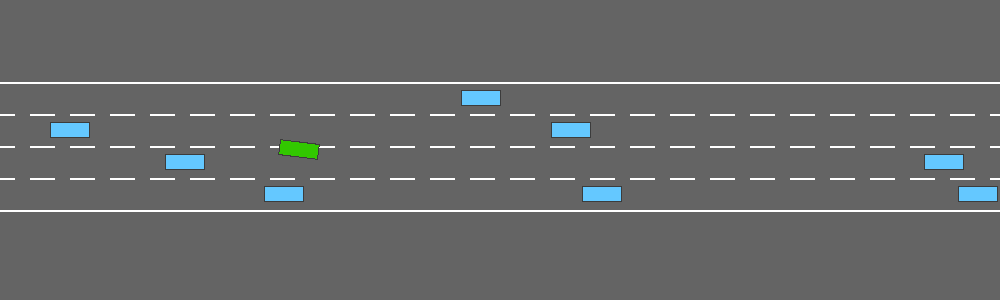
\includegraphics[width=\columnwidth]{img/highway}\caption{Highway}\end{subfigure}&
		\begin{subfigure}{0.49\textwidth}\centering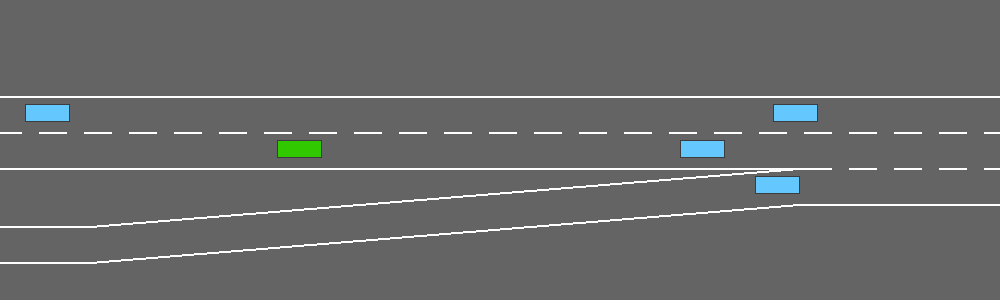
\includegraphics[width=\columnwidth]{img/merge}\caption{Merge}\end{subfigure}\\
		\newline
		\begin{subfigure}{0.49\textwidth}\centering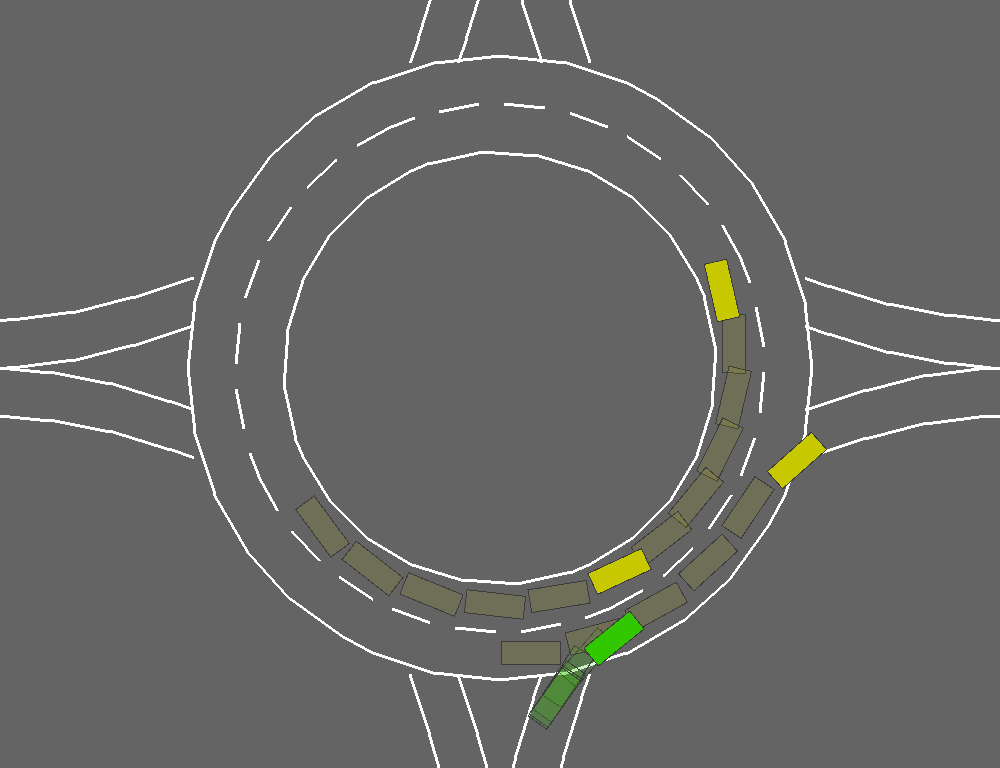
\includegraphics[width=\columnwidth]{img/roundabout}\caption{Roundabout}\end{subfigure}&
		\begin{subfigure}{0.49\textwidth}\centering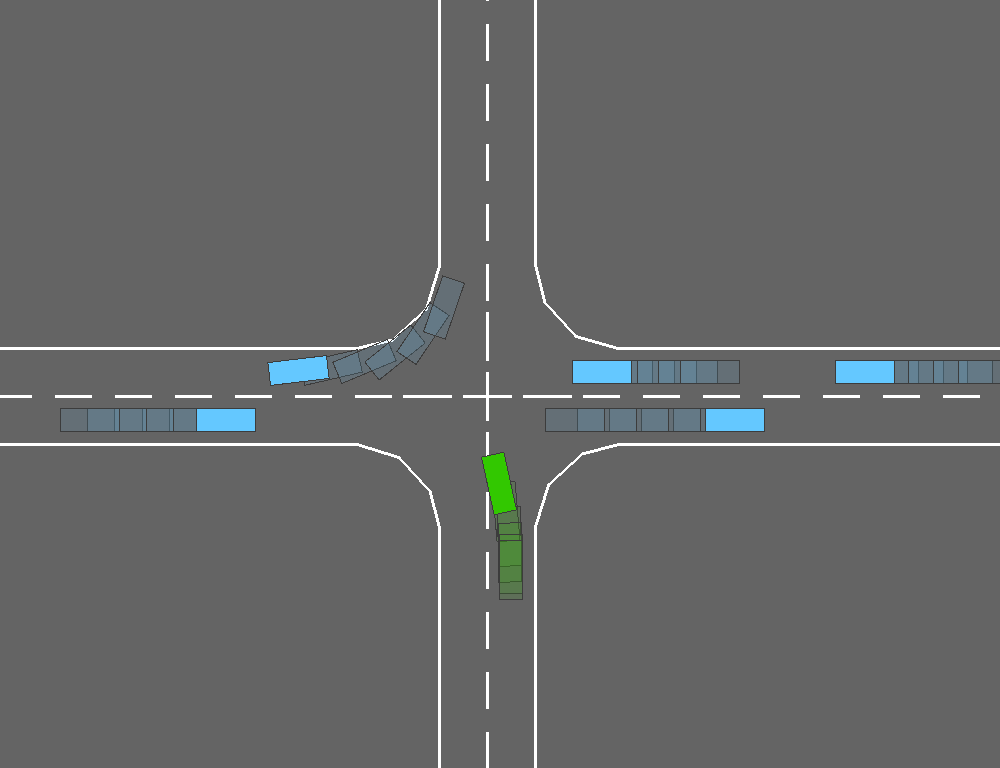
\includegraphics[width=\columnwidth]{img/intersection}\caption{Intersection}\end{subfigure}\\
		\begin{subfigure}{0.49\textwidth}\centering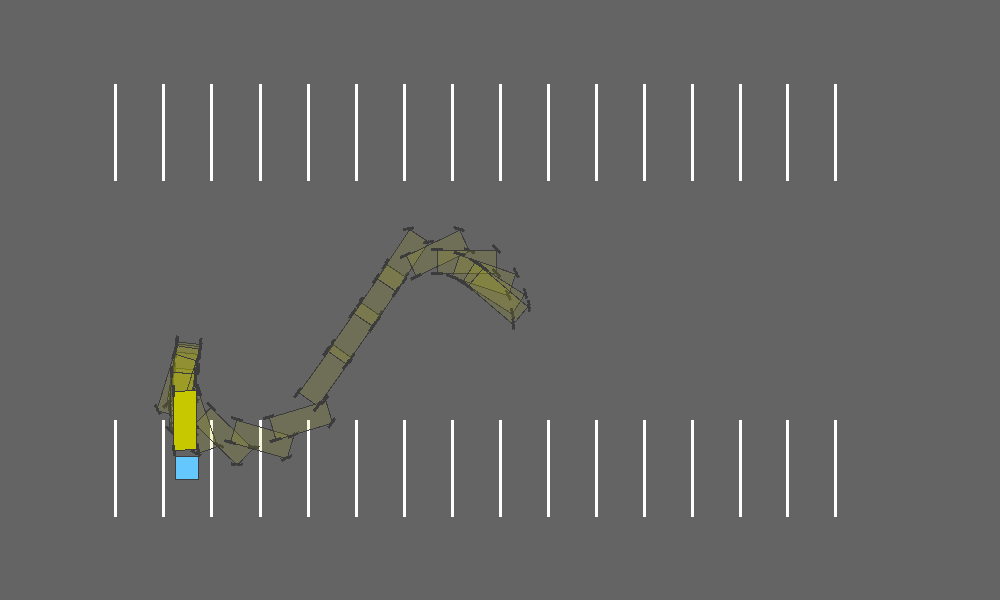
\includegraphics[width=\columnwidth]{img/parking}\caption{Parking}\end{subfigure}&
		\begin{subfigure}{0.49\textwidth}\centering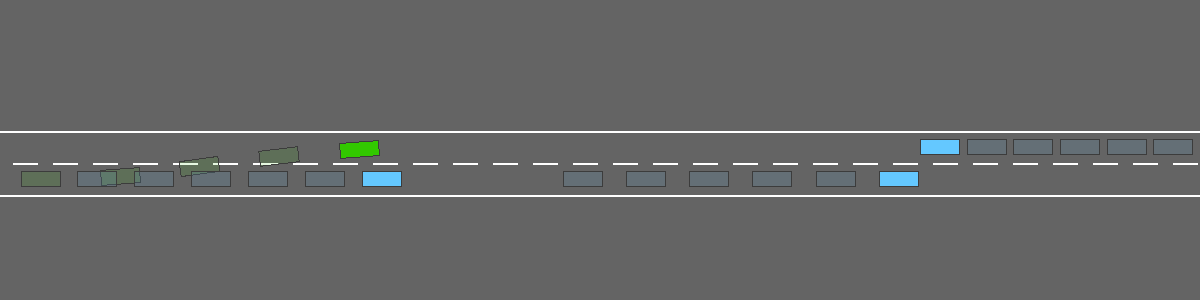
\includegraphics[width=\columnwidth]{img/two-way}\caption{Two-way}\end{subfigure}\\
	\end{tabular}
	\caption{The different environments available in \textsc{highway-env}.}
	\label{tab:environments}
\end{table}

\begin{itemize}
	\item \textbf{Highway.} The vehicle is driving on a highway populated with other drivers. The goal is to drive as fast as possible while avoiding collisions with other vehicles, through a discrete meta-action space of manoeuvres.
	\item \textbf{Merge.} The task is similar to \texttt{highway-v0}, but a vehicle is incoming from an access ramp and must be able to merge successfully in traffic. To that end, the ego-vehicle must change lane or adapt its velocity so that the merging vehicle has sufficient space. This task is inspired by a practical use case for \gls{ADAS} systems at Renault.
	\item \textbf{Roundabout.} The vehicle must cross a roundabout as fast as possible while avoiding collisions. It requires reasoning about the uncertain destinations of other vehicles.
	\item \textbf{Intersection.} This environment is similar to roundabout, but with an increased density of vehicles and types of conflicts. Only the throttle is controlled, and the steering is performed automatically to track the ego-vehicle destination.
	\item \textbf{Parking.} A goal-conditioned continuous control environment: the desired parking spot location is part of the observation, and the ego-vehicle must plan cusp-shaped manoeuvres to reach it with the proper heading.
	\item \textbf{Two-way.} This environment is similar to highway, except that the ego-vehicle can change to a lane facing the opposite direction, with incoming vehicles. This enables to highlight an efficiency-safety trade-off for risk-sensitive decision-making.
\end{itemize}

\paragraph{Features}

Several parts of the environment can be configured.

\begin{itemize}
	\item \textbf{Observations.} Several types of observations are available, such as the \emph{list of features} and \emph{occupancy grid} described in \Cref{chapter:4}. Other types include RGB images, time-to-collision maps, and goal locations.
	\item \textbf{Actions.} In addition to the discrete meta-action space $\cA$ described in \Cref{chapter:3}, a continuous space $\cA=\Real^2$ for throttle and steering can also be selected.
	\item \textbf{Dynamics.} Other vehicles can follow the \gls{IDM} and \gls{MOBIL} behavioural models as described in  \Cref{chapter:3} or its linearised version of \Cref{sec:prediction}. The ego-vehicle can be controlled with either the Kinematic Bicycle Model as in \Cref{chapter:3} or the Dynamic Bicycle Model as in  \Cref{sec:robust-stabilisation}.
	\item \textbf{Rewards.} The rewards and penalties associated with speed or collisions are configurable.
	\item \textbf{Graphics.} Graphics are rendered using the \href{https://www.pygame.org/news}{pygame} library, window size and resolution can be configured.
\end{itemize} 


\paragraph{Development process}

The project closely follows the insights of \Cref{chapter:3} in its definition of the traffic state, actions, dynamics, and rewards. See the \href{https://highway-env.readthedocs.io/en/latest/user\_guide.html}{user guide} in the documentation for more details.

It also complies by the \href{https://github.com/openai/gym}{OpenAI gym} standard interface for \gls{RL} environments. Continuous integration (CI) is performed with \href{https://docs.pytest.org/en/stable/}{pytest} unit tests automatically triggered with \href{https://github.com/features/actions}{GitHub actions}. The documentation is built from the source code comments using \href{https://www.sphinx-doc.org/en/master/}{Sphinx}, and hosted on \href{https://readthedocs.org/}{Read the Docs}. Finally, multiple examples can be run directly from the browser through \href{https://colab.research.google.com/}{Google Colab} notebooks.

\section{Outreach}
\label{sec:outreach}
In this section, we document the dissemination of the library among several communities.

\subsection{Academia}

We highlight that several researchers have reported using or referred to \textsc{highway-env} in their publications and submissions:
\begin{itemize}
	\item \fullcite{Li2019}
	\item \fullcite{Yang2020}
	\item \fullcite{n2020smart}
	\item \fullcite{Xu2020taskagnostic}
	\item \fullcite{ma2020dsac}
	\item \fullcite{mei2020prioritized}
	\item \fullcite{zhang2020bi}
	\item \fullcite{mavrogiannis2020bgap}
	\item \fullcite{zhou2020smarts}
	\item \fullcite{terry2020pettingzoo}
	\item \fullcite{kapoor2020modelbased}
	\item \fullcite{Zhang2020Spatial}
	\item \fullcite{mei2020prioritized}
\end{itemize}

\leavevmode\newline
Additionally, we use it in most of our own publications:
\begin{itemize}
	\item \fullcite{Leurent2018approximate}
	\item \fullcite{Leurent2019interval}
	\item \fullcite{Leurent2019social}
	\item \fullcite{CarraraLeurent2019}
	\item \fullcite{Leurent2020practical}
	\item \fullcite{Leurent2020robust}
	\item \fullcite{Leurent2020beyond}
\end{itemize}

\leavevmode\newline
\noindent Finally, the \textsc{highway-env} library is featured in the documentation and examples of two of the most famous libraries in the \gls{RL} ecosystem:
\begin{itemize}
\item \href{https://github.com/openai/gym}{OpenAI Gym}, a standard interface for comparing \gls{RL} algorithms. \textsc{highway-env} is mentioned in the \href{https://github.com/openai/gym/blob/master/docs/environments.md#highway-env-tactical-decision-making-for-autonomous-driving}{list of environments}.
\item \href{https://github.com/hill-a/stable-baselines}{Stable Baselines}, a set of improved implementations of \gls{RL} algorithms based on OpenAI Baselines. \textsc{highway-env} is used as an  \href{https://stable-baselines.readthedocs.io/en/master/guide/examples.html#hindsight-experience-replay-her}{example} in the documentation.
\end{itemize}

\subsection{Education}

Since the publication of \textsc{highway-env}, many masters students have contacted me throughout the years, and reported using the simulator for their final project of in various courses, occasionally upon suggestion by their professor.
I did not keep track of all these exchanges, but as a trace of this activity, see:
\begin{itemize}
	\item the \href{https://github.com/eleurent/highway-env/issues?q=is\%3Aissue}{list of issues} opened in \textsc{highway-env}.
	\item the \href{https://github.com/eleurent/rl-agents/issues?q=is\%3Aissue}{list of issues} opened in \textsc{rl-agents}.
\end{itemize} 

\subsection{Industry}

Several engineers, mainly from the Automotive industry, have demonstrated interest in \textsc{highway-env}, either by reaching out to me directly or by developing their own project on top of the library. To name a few,

\begin{itemize}
    \item \href{https://www.linkedin.com/in/simon-chauvin/}{Simon Chauvin}, Machine Learning Engineer at Autonomous Driving at \href{https://www.esrlabs.com/}{ESR Labs AG}, who contacted me to reproduce my results.
	\item \href{https://www.linkedin.com/in/huberclement}{Clément Huber}, Product Owner in the Path Planning team at \href{https://navya.tech/fr/}{NAVYA Group}, and \href{https://www.linkedin.com/in/lucas-boyer}{Lucas Boyer}, intern in that team, contacted me on several occasions to discuss the \href{https://github.com/lucasBOYER/highway-env}{internship} of Lucas based on \textsc{highway-env} and \textsc{openai/baselines}.
	\item \href{https://www.linkedin.com/in/munirjojoverge}{Munir Jojo-Verge}, Motion Planning and Decision Making Manager at \href{https://canvas.technology/}{Amazon Robotics}, who wrote to me regarding his extension of \textsc{highway-env} to continuous actions, see \href{https://github.com/munirjojoverge/rl_AD_urban_baselines}{his fork} which lead to the addition of the \texttt{parking-v0} environment.
	\item \href{https://www.linkedin.com/in/deepdrive}{Craig Quiter}, Founder of \href{https://deepdrive.voyage.auto/}{Deepdrive} at \href{https://voyage.auto/}{Voyage}, who mentioned that \href{https://medium.com/@crizcraig/smooth-operator-92c6c14862fb}{his recent work} was inspired by \textsc{highway-env} and with whom I had the pleasure to discuss.
	\item \href{https://www.linkedin.com/in/pinaki-gupta/}{Pinaki Gupta}, Behaviour Planning architect at \href{https://lucidmotors.com/}{Lucid Motors}, see \href{https://github.com/pinakigupta/BehaviorRL}{his fork} that features variants of the \texttt{two-way-v0} and \texttt{parking-v0} environments augmented with additional vehicles and multiple goals.
	\item \href{https://www.linkedin.com/in/guillaumealleon}{Guillaume Alleon}, Head of AI research at \href{https://www.airbus.com/}{Airbus}, see \href{https://github.com/galleon/highway-env}{his fork}.
    \item \href{https://ru.linkedin.com/in/boris-yangel-83194729}{Boris Yangel}, Principal Software Engineer at \href{https://yandex.com/}{Yandex}, see \href{https://github.com/hr0nix/trackdays/blob/master/setup.py}{his project}.
\end{itemize}


 



	%!TEX root = ../../PhD_thesis__Edouard_Leurent.tex
\graphicspath{{2-Chapters/5-Chapter/}}

\chapter{Complements on \Cref{chapter:5}}
\section{Proofs}
\label{sec:proofs}
\subsection{Proof of \Cref{prop:bellman-expectation}}
\label{sec:proof-bell-expect}
\begin{proof}
	Thanks to the introduction of the augmented spaces $\ocS, \ocA$ and dynamics $\augmentedtransition$, this proof is the same as that in classical \glspl{MOMDP}.
	\begin{align*}
	\oV^{\budgetedpolicy}(\os) &\eqdef \expectedvalue\left[ \augmentedreturn^{\budgetedpolicy} \condbar \ov{s_0} = \os\right] \\
	&=\sum_{\oa\in\ocA} \probability{\oa_0 = \oa \condbar\ov{s_0} = \os} \expectedvalue\left[ \augmentedreturn^{\budgetedpolicy} \condbar \ov{s_0} = \os, \oa_0 = \oa\right]\\
	&= \sum_{\oa\in\ocA} \budgetedpolicy(\oa | \os) \oQ^{\budgetedpolicy}(\os,\oa).
	\end{align*}
	
	\begin{align*}
	\oQ^{\budgetedpolicy}(\os, \oa) &\eqdef \expectedvalue\left[\sum_{t=0}^\infty \discountfactor^t \augmentedreward(\os_t, \oa_t)\condbar \ov{s_0} = \os, \ov{a_0} = \oa\right] \\
	&= \augmentedreward(\os, \oa) + \sum_{\os'\in\ocS}\probability{\os_1 = \os' \condbar\ov{s_0} = \os, \ov{a_0} = \oa}\cdot \expectedvalue\left[\sum_{t=1}^\infty \discountfactor^t \augmentedreward(\os_t, \oa_t)\condbar \ov{s_1} = \os'\right] \\
	&= \augmentedreward(\os, \oa) + \discountfactor\sum_{\os'\in\ocS}\augmentedtransition\left(\os' \condbar\os, \oa\right) \expectedvalue\left[\sum_{t=0}^\infty \discountfactor^t \augmentedreward(\os_t, \oa_t) \condbar \ov{s_0} = \os'\right] \\
	&= \augmentedreward(\os, \oa) + \discountfactor\sum_{\os'\in\ocS}\augmentedtransition\left(\os' \condbar\os, \oa\right) \oV^{\budgetedpolicy}(\os').
	\end{align*}
	
	\paragraph{Contraction of $\abo^{\budgetedpolicy}$.}
	Let $\budgetedpolicy\in\policies, \oQ_1, \oQ_2\in(\Real^2)^{\ocS\ocA}$.
	\begin{align*}
	\forall \os\in\ocS, \oa\in\ocA,\quad \left|\abo^{\budgetedpolicy} \oQ_1(\os,\oa) - \abo^{\budgetedpolicy} \oQ_2(\os,\oa)\right| &= \left|\discountfactor\expectedvalueover{\substack{\os'\sim\augmentedtransition(\os'|\os,\oa) \\ \oa'\sim\budgetedpolicy(\oa'|\os')}} \oQ_1(\os',\oa') - \oQ_2(\os',\oa')\right|\\
	&\leq \discountfactor\left\|\oQ_1-\oQ_2\right\|_\infty.
	\end{align*}
	Hence, $\left\|\abo^{\budgetedpolicy} \oQ_1 - \abo^{\budgetedpolicy} \oQ_2 \right\|_\infty \leq \discountfactor\left\|\oQ_1-\oQ_2\right\|_\infty$
	
	According to the Banach fixed point theorem \citep{Banach1922}, $\abo^{\budgetedpolicy}$ admits a unique fixed point.
	It can be easily verified that $\oQ^{\budgetedpolicy}$ is indeed this fixed point by combining the two Bellman Expectation equations~\eqref{eq:bellman_expectation}.
	
\end{proof}

\subsection{Proof of \Cref{thm:bellman-optimality}}
\label{sec:proof-bell-optim}

\begin{proof}
    Let $\os, \oa \in \ocA\times\ocS$. For this proof, we consider potentially non-stationary policies $\budgetedpolicy=(\rho, \budgetedpolicy')$, with $\rho\in\cM(\ocA)$, $\budgetedpolicy'\in\cM(\ocA)^\Natural$. The results will apply to the particular case of stationary optimal policies, when they exist.
    \begin{align}
        \Qr[^\star](\os, \oa) &=  \max_{\rho, \budgetedpolicy'} \Qr[^{\rho, \budgetedpolicy'}](\os', \oa') \label{eq:pthm_def}\\
        &= \max_{\rho, \budgetedpolicy'} \reward(s, a) + \discountfactor \sum_{\os'\in\ocS} \augmentedtransition(\os' | \os, \oa) \Vr[^{\rho, \budgetedpolicy'}](\os') \label{eq:pthm_exp}\\
        &= \reward(s, a) + \discountfactor \sum_{\os'\in\ocS}  \augmentedtransition(\os' | \os, \oa) \max_{\rho, \budgetedpolicy'} \sum_{\oa'\in\ocA} \rho(\oa' | \os')\Qr[^{\budgetedpolicy'}](\os', \oa') \label{eq:pthm_marg}\\
        &= \reward(s, a) + \discountfactor \sum_{\os'\in\ocS}  \augmentedtransition(\os' | \os, \oa) \max_\rho\sum_{\oa'\in\ocA}\rho(\oa' | \os')\max_{\budgetedpolicy'\in\policies_a(\os')}\Qr[^{\budgetedpolicy'}](\os', \oa') \label{eq:pthm_max}\\
        &= \reward(s, a) + \discountfactor \sum_{\os'\in\ocS}  \augmentedtransition(\os' | \os, \oa) \max_\rho\expectedvalueover{\oa'\sim\rho}\Qr[^\star](\os', \oa') \label{eq:pthm_marg_def2}
    \end{align}
    where $\budgetedpolicy = (\rho, \budgetedpolicy')\in\policies_a(\os)$ and $\budgetedpolicy'\in\policies_a(\os')$.

    This follows from:
    \begin{enumerate}
        \item[\eqref{eq:pthm_def}.] Definition of $\oQ^{\star}$.
        \item[\eqref{eq:pthm_exp}.] Bellman Expectation expansion from \Cref{prop:bellman-expectation}.
        \item[\eqref{eq:pthm_marg}.] Marginalisation on $\oa'$.
        \item[\eqref{eq:pthm_max}.] \begin{itemize}
            \item Trivially $\max_{\budgetedpolicy'\in\policies_a(\os')} \sum_{\oa'\in\ocA} \cdot \leq \sum_{\oa'\in\ocA} \max_{ \budgetedpolicy'\in\policies_a(\os)} \cdot$.
            \item Let $\ov{\budgetedpolicy}\in\argmax_{\budgetedpolicy'\in\policies_a(\os')} \Qr[^{\budgetedpolicy'}](\os', \oa')$, then:
            \begin{align*}
                \sum_{\oa'\in\ocA}\rho(\oa'|\os')\max_{\budgetedpolicy'\in\policies_a(\os')}\Qr[^{\budgetedpolicy'}](\os', \oa') &= \sum_{\oa'\in\ocA}\rho(\oa'|\os')\Qr[^{\budgetedpolicy'}](\os', \oa') \\
                &\leq  \max_{\budgetedpolicy'\in\policies_a(\os')} \sum_{\oa'\in\ocA}\rho(\oa'|\os')\Qr[^{\budgetedpolicy'}](\os', \oa').
            \end{align*}
        \end{itemize}
        \item[\eqref{eq:pthm_marg_def2}.] Definition of $\oQ^{\star}$.
    \end{enumerate}

    Moreover, the condition $\budgetedpolicy=(\rho, \budgetedpolicy')\in\policies_a(\os)$ gives
    \begin{equation*}
        \expectedvalueover{\oa'\sim\rho} \Qc[^{\star}](\os, \oa) = \expectedvalueover{\oa'\sim\rho} \Qc[^{\budgetedpolicy'}](\os, \oa) = \Vc[^{\budgetedpolicy}](\os) \leq \budget.
    \end{equation*}

    Consequently, $\budgetedpolicy_\text{greedy}(\cdot; \oQ^{\star})$ belongs to the $\argmax$ of \eqref{eq:pthm_marg_def2}, and in particular:
    \begin{equation*}
        \Qr[^{\star}](\os, \oa) = r(\os, \oa) + \discountfactor \sum_{\os'\in\ocS}  P(\os' | \os, \oa) \expectedvalueover{\oa'\sim\budgetedpolicy_\text{greedy}(\os', \oQ^{\star})} \Qr[^{\star}](\os', \oa').
    \end{equation*}

    The same reasoning can be made for $\Qc[^\star]$ by replacing $\max$ operators by $\min$, and $\policies_a$ by $\policies_r$.
\end{proof}


\subsection{Proof of \Cref{prop:greedy_optimal}}
\label{sec:proof-greedy-optim}
\begin{proof}
    Notice from the definitions of $\abo^{\star}$ and $\abo^{\budgetedpolicy}$ in \eqref{eq:bellman-optimality} and \eqref{eq:bellman_expectation_operator} that $\abo^{\star}$ and $\abo^{\budgetedpolicy_\text{greedy}(\cdot;\oQ^{\star})}$ coincide on $\oQ^{\star}$. Moreover, since $\oQ^{\star} = \abo^{\star}\oQ^{\star}$ by \Cref{thm:bellman-optimality}, we have: $\abo^{\budgetedpolicy_\text{greedy}(\cdot;\oQ^{\star})} \oQ^{\star} = \abo^{\star} \oQ^{\star} = \oQ^{\star}$.
    Hence, $\oQ^{\star}$ is a fixed point of $\abo^{\budgetedpolicy_\text{greedy}(\cdot;\oQ^{\star})}$, and by \Cref{prop:bellman-expectation} it must be equal to $\oQ^{\budgetedpolicy_\text{greedy}(\cdot;\oQ^{\star})}$

    To show the same result for $\oV^{\star}$, notice that
    \begin{equation*}
        \oV^{\budgetedpolicy_\text{greedy}(\oQ^{\star})}(\os) = \expectedvalueover{\oa\sim\budgetedpolicy_\text{greedy}(\oQ^{\star})}\oQ^{\budgetedpolicy_\text{greedy}(\oQ^{\star})}(\os,\oa) = \expectedvalueover{\oa\sim\budgetedpolicy_\text{greedy}(\oQ^{\star})}\oQ^{\star}(\os,\oa).
    \end{equation*}
    By applying the definitions of $\oQ^{\star}$ and $\budgetedpolicy_\text{greedy}$, we recover the definition of $\oV^{\star}$.
\end{proof}

\subsection{Proof of \Cref{thm:contraction}}
\label{sec:proof-contraction}
\begin{proof}
	In the trivial case $|\cA| = 1$, there exits only one policy $\budgetedpolicy$ and $\abo = \abo^\budgetedpolicy$, which is a contraction by \Cref{prop:bellman-expectation}.
	
	In the general case $|\cA| \geq 2$, we can build the following counter-example.
	
	Let $(\cS, \cA, P, R_r, R_c)$ be a \gls{BMDP}.
	For any $\epsilon > 0$, we define $\oQ_\epsilon^1$ and $\oQ_\epsilon^2$ as
	\begin{align*}
	\oQ_\epsilon^1(\os,\oa) =
	\begin{cases}
	(0, 0), & \text{if } a = a_0 \\
	\left(\frac{1}{\discount}, \epsilon\right), & \text{if } a \neq a_0
	\end{cases}\\
	\oQ_\epsilon^2(\os,\oa) =
	\begin{cases}
	(0, \epsilon), & \text{if } a = a_0 \\
	\left(\frac{1}{\discount}, 2\epsilon\right), & \text{if } a \neq a_0
	\end{cases}
	\end{align*}
	Then, $\|\oQ_1-\oQ_2\|_\infty = \epsilon$.
	$\oQ_\epsilon^1$ and $\oQ_\epsilon^2$ are represented in \Cref{fig:concavity_example}.
	
	\begin{figure}[tp]
		\centering
		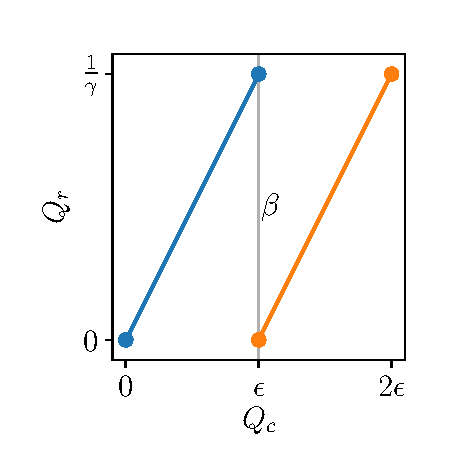
\includegraphics[width=0.4\textwidth]{img/concavity_example.pdf}
		\caption{Representation of $\oQ_\epsilon^1$ (blue) and $\oQ_\epsilon^2$ (yellow)}
		\label{fig:concavity_example}
	\end{figure}
	
	But for $\oa=(a,\budgetaction)$ with $\budgetaction = \epsilon$, we have
	\begin{align*}
	\|\abo \oQ_\epsilon^1(\os, \oa) - \abo \oQ_\epsilon^2(\os, \oa)\|_\infty &= \discount\left\|\expectedvalueover{\os'\sim\augmentedtransition(\os'|\os,\oa)} \expectedvalueover{\oa'\sim\budgetedpolicy_\text{greedy}(\oQ^1_\epsilon)}\oQ^1_\epsilon(\os',\oa') - \expectedvalueover{\oa'\sim\budgetedpolicy_\text{greedy}(\oQ^2_\epsilon)}\oQ^2_\epsilon(\os',\oa')\right\|_\infty \\
	&= \discount\left\|\expectedvalueover{\os'\sim\augmentedtransition(\os'|\os,\oa)}\left(\frac{1}{\discount}, \epsilon\right) - (0, \epsilon)\right\|_\infty \\
	&= \discount\frac{1}{\discount} = 1
	\end{align*}
	Hence, 
	\begin{align*}
	\|\abo \oQ_\epsilon^1 - \abo \oQ_\epsilon^2\|_\infty &\geq 1 = \frac{1}{\epsilon} \|\oQ_1-\oQ_2\|_\infty
	\end{align*}
	
	In particular, there does not exist $L>0$ such that
	$$\forall \oQ_1,\oQ_2\in(\Real^2)^{\ocS\ocA}, \|\abo \oQ^1 - \abo \oQ^2\|_\infty \leq L \|\oQ^1 - \oQ^2\|_\infty$$
	In other words, $\abo$ is not a contraction for $\|\cdot\|_\infty$.
\end{proof}

\subsection{Proof of \Cref{thm:contractivity-smooth}}
\label{sec:contraction-with-smooth}

\begin{remark}
	\begin{leftbar}[remarkbar]
	This proof makes use of insights detailed in the proof of \Cref{prop:bftq_pi_hull} (\Cref{sec:proof_pi_hull}), which we recommend the reader to consult first.
	\end{leftbar}
\end{remark}

\begin{proof}
	We now study the contractivity of $\abo^{\star}$ when restricted to the functions of $\cL_{\discountfactor}$ defined as follows:
    \begin{equation}
    \cL_{\discountfactor} = \left\{\begin{array}{cc}
   \oQ\in(\Real^2)^{\ocS\ocA}\text{ s.t. }\exists L<\frac{1}{\discountfactor}-1: \forall \os\in\ocS,\oa_1,\oa_2\in\ocA,   \\
   |\Qr(\os,\oa_1) - \Qr(\os,\oa_2)| \leq L|\Qc(\os,\oa_1) - \Qc(\os,\oa_2)|
    \end{array}\right\}.
    \end{equation}
    That is, for all state $\os$, the set $\oQ(\os, \ocA)$ plot in the $(\Qc,\Qr)$ plane must be the \emph{graph} of a $L$-Lipschitz function, with $L<1/\discountfactor-1$.

    We impose such structure for the following reason: the counter-example presented above prevented contraction because it was a pathological case in which the slope of $\oQ$ can be arbitrary large. As a consequence, when solving $\Qr[^\star]$ such that $\Qc[^\star]=\budget$, a vertical slice of a $\|\cdot\|_\infty$ ball around $\oQ_1$ (which must contain $\oQ_2$) can be arbitrary large as well.


    We denote $\text{Ball}(\oQ,R)$ the ball of centre $\oQ$ and radius $R$ for the $\|\cdot\|_\infty$-norm:
    \begin{equation*}
        \text{Ball}(\oQ,R) = \{\oQ'\in(R^2)^{\ocS\ocA}: \|\oQ-\oQ'\|_\infty \leq R\}.
    \end{equation*}

    We give the three main steps required to show that $\abo^{\star}$ restricted to $\cL_{\discountfactor}$ is a contraction. Given $\oQ^1, \oQ^2\in\cL_{\discountfactor}$, show that:

    \begin{enumerate}
        \item $\oQ^2\in\text{Ball}(\oQ^1,R)\implies\cF^2\in\text{Ball}(\cF^1, R), \forall\os\in\ocS$, where $\cF$ is the top frontier of the convex hull of undominated points, as defined in~\Cref{sec:proof_pi_hull}.
        \item $\oQ\in\cL_{\discountfactor} \implies \cF$ is the graph of a $L$-Lipschitz function, $\forall\os\in\ocS$.
        \item taking the slice $\Qc=\budget$ of a ball $\text{Ball}(\cF,R)$ with $\cF$ $L$-Lipschitz results in an interval on $\Qr$ of range at most $(L+1)R$
    \end{enumerate}
	
	These three steps will allow us to control $\Qr[^{2\star}] - \Qr[^{1\star}]$ as a function of $R = \|\oQ^2-\oQ^1\|_\infty$.

    \paragraph{Step 1}

    We want to show that if $\oQ^1$ and $\oQ^2$ are close, then $\cF^1$ are $\cF^2$ are close as well in the following sense:
    \begin{align}
        \cF^2\in\text{Ball}(\cF^1, R) &\iff d(\cF^1, \cF^2) \leq R \iff \max_{q^2\in\cF^2}\min_{q^1\in\cF^1}\|q^2-q^1\|_\infty \leq R.
        \label{eq:ball-set}
    \end{align}

    Assume $\oQ^2\in\text{Ball}(\oQ^1,R)$, we show by contradiction that $\cF^2 \in \text{Ball}(\cF^1, R)$. Indeed, assume there exists $q^1\in \cF^1$ such that $\cF^2 \cap \text{Ball}(q^1, R) = \emptyset$. Denote $q^2$ the unique point of $\cF^2$ such that $q^2_c = q^1_c$. By construction of $q^1$, we know that $\|q^1-q^2\|_\infty > R$. There are two possible cases:
    \begin{itemize}
        \item $q^2_r > q^1_r$: this also directly implies that $q^2_r > q^1_r + R$. But $q^2\in\cF^2$, so there exist $q^2_1, q^2_2\in Q^{2},\lambda\in\Real$ such that $q^2 = (1-\lambda)q^2_1 + \lambda q^2_2$. But since $\oQ^2\in \text{Ball}(\oQ^1, R)$, there also exist $q_1^1, q^1_2\in \oQ^1$ such that $\|q^1_1-q^2_1\|_\infty \leq R$ and $\|q^1_2-q^2_2\|_\infty \leq R$, and in particular $q^1_{1r}\geq q^2_{1r}-R$ and $q^1_{2r}\geq q^2_{2r}-R$. But then, the point $q^{1'}=(1-\mu)q^1_1 + \mu q^1_2$ with $\mu=(q^2_c-q^1_{1c})/(q^2_{2c}-q^1_{1c})$ verifies $q^{1'}_c = q^1_c$ and $q^{1'}_r \geq q^2_r - R > q^1_r$ which contradicts the definition of $q_1\in\cF^1$ as defined in \eqref{eq:top-frontier}.
        \item $q^2_r < q^1_r$: then the same reasoning can be applied by simply swapping the indexes 1 and 2.
    \end{itemize}

    % We start by showing this result for $\cC^2(Q^{1-})$ and $\cC^2(Q^{2-})$ as defined in \Cref{sec:proof_pi_hull}:
    % Let $\os\in\ocS$ and $q^2\in\cC^2(Q^{2-})$, $\exists\lambda\in[0,1], \oa_1,\oa_2\in\ocA: q^2 = (1-\lambda)Q^2(\os,\oa_1) + \lambda Q^2(\os,\oa_2)$. Define $q^1 = (1-\lambda)Q^1(\os,\oa_1) + \lambda Q^1(\os,\oa_2)$. Then
    % \begin{align*}
    %     \|q^2-q^1\|_\infty &= \|(1-\lambda)(Q^2(\os,\oa_1) - Q^1(\os,\oa_1)) + \lambda (Q^2(\os,\oa_2) - Q^1(\os,\oa_2))\|_\infty\\
    %     &\leq  (1-\lambda)\|Q^2(\os,\oa_1) - Q^1(\os,\oa_1)\|_\infty + \lambda \|Q^2(\os,\oa_2) - Q^1(\os,\oa_2)\|_\infty\\
    %     &\leq (1-\lambda)R+\lambda R = R
    % \end{align*}

    % It remains to show that when taking the top frontiers of the convex sets $\cC^2(Q^{1-})$ and $\cC^2(Q^{2-})$, they remain at a distance of at most $R$.

    We have shown that $\cF^2 \in \text{Ball}(\cF^1, R)$.
    This is illustrated in \Cref{fig:contraction_lips_hull}: given a function $\oQ^1$, we show the locus $\text{Ball}(\oQ_1,R)$ of $\oQ^2$. We then draw $\cF^1$ the top frontier of the convex hull of $\oQ^1$ and alongside the locus of all possible $\cF^2$, which belong to a ball $\text{Ball}(\cF^1, R)$.

    \begin{figure}[ht]
        \centering
        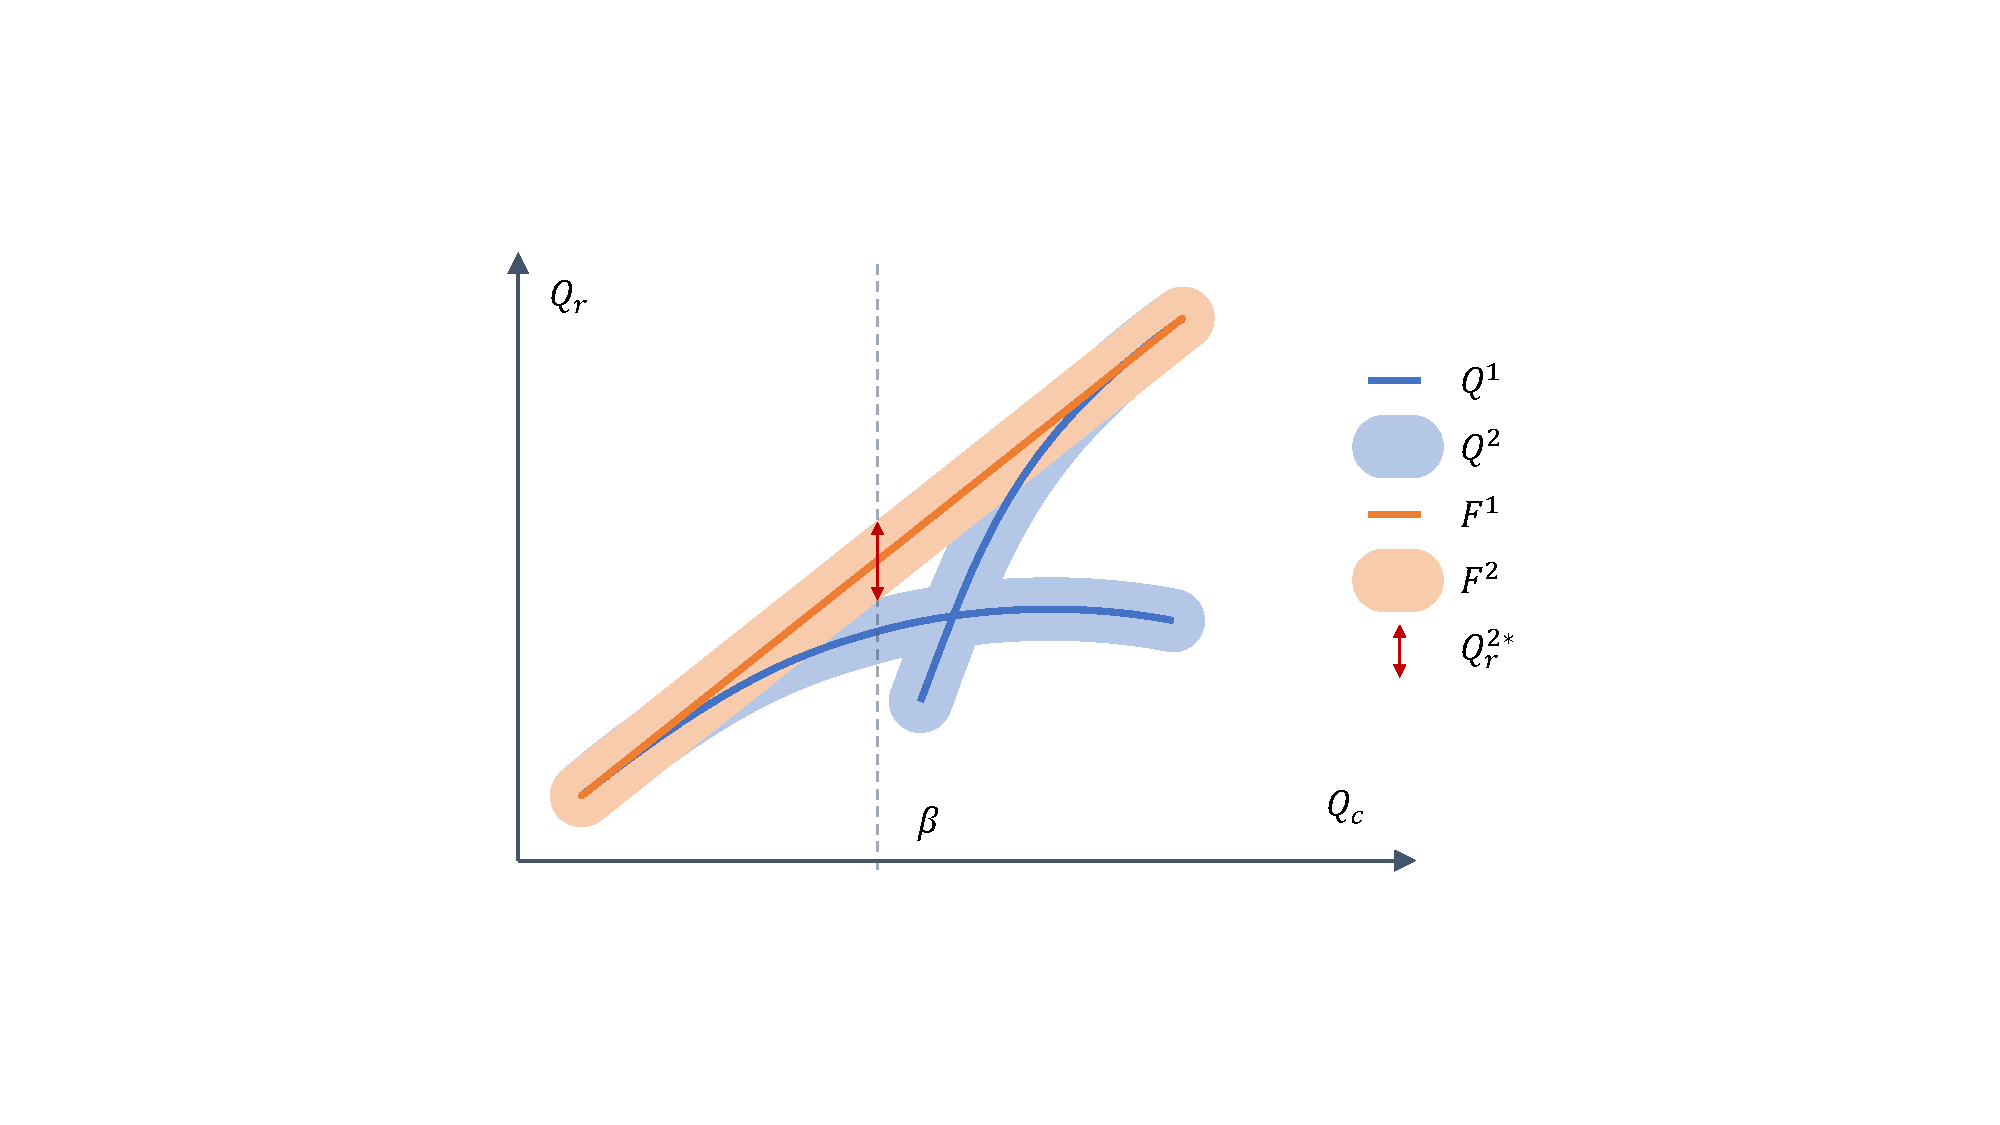
\includegraphics[trim=7cm 4cm 7cm 4cm, clip, width=0.7\textwidth]{img/contraction_lipschitz.pdf}
        \caption{We represent the range of possible solutions $\Qr[^{2\star}]$ for any $\oQ^2\in\text{Ball}(\oQ^1)$, given $\oQ_1\in\cL_\lambda$}
        \label{fig:contraction_lips_hull}
    \end{figure}

    \paragraph{Step 2}

    We want to show that if $\oQ\in\cL_{\discountfactor}$, $\cF$ is the graph of an $L$-Lipschitz function:
    \begin{equation}
        \label{eq:L-lip-set}
        \forall q^1,q^2\in\cF, |q_r^2-q_r^1| \leq |q_c^2-q_c^1|.
    \end{equation}

    Let $\oQ\in\cL_{\discountfactor}$ and $\os\in\ocS$, $\cF$ the corresponding top frontier of convex hull.
    For all $q^1,q^2\in\cF, \exists \lambda,\mu\in[0,1], q^{11},q^{12},q^{21},q^{22}\in \oQ(\os,\ocA)$ such that $q^1 = (1-\lambda)q^{11} + \lambda q^{12}$ and $q^2 = (1-\mu)q^{21} + \mu q^{22}$.
    Without loss of generality, we can assume $q_c^{11}\leq q_c^{12}$ and $q_c^{21}\leq q_c^{22}$. We also consider the worst case in terms of maximum $q_r$ deviation: $q_c^{12} \leq q_c^{21}$.
    Then the maximum increment $q_r^2-q_r^{1}$ is:
    \begin{align*}
        \|q^2_r-q^{1}_r\| &\leq \|q^{12}_r-q^{1}_r\| + \|q^{21}_r-q^{12}_r\| + \|q^{2}_r-q^{21}_r\| \\
        &= (1-\lambda)\|q^{12}_r-q^{11}_r\| + \|q^{21}_r-q^{12}_r\| + \mu\|q^{22}_r-q^{21}_r\| \\
        &\leq (1-\lambda)L\|q^{12}_c-q^{11}_c\| + L\|q^{21}_c-q^{12}_c\| + \mu L\|q^{22}_c-q^{21}_c\| \\
        &= L\|q^{12}_c-q^{1}_c\| + L\|q^{21}_c-q^{12}_c\| + L\|q^{2}_c-q^{21}_c\|\\
        &= L\|q^{2}_c-q^{1}_c\|.
    \end{align*}

    This can also be seen in \Cref{fig:contraction_lips_hull}: the maximum slope of the $\cF^1$ is lower than the maximum slope between two points of $\oQ^1$.

    \paragraph{Step 3}

    Let $\cF_1$ be a L-Lipschitz set as defined in \eqref{eq:L-lip-set}, and consider a ball $\text{Ball}(\cF_1,R)$ around it as defined in \eqref{eq:ball-set}.

    We want to bound the optimal reward value $\Qr[^{2\star}]$ under constraint $\Qc[^{2\star}] = \budget$ (regular case in \Cref{sec:proof_pi_hull} where the constraint is saturated), for any $\cF^2\in\text{Ball}(\cF_1,R)$. This quantity is represented as a red double-ended arrow in \Cref{fig:contraction_lips_hull}.

    Because we are only interested in what happens locally at $\Qc=\budget$, we can zoom in on \Cref{fig:contraction_lips_hull} and only consider a thin $\epsilon$-section around $\budget$. In the limit $\epsilon\rightarrow 0$, this section becomes the tangent to $\cF^1$ at $\Qc[^1]=\budget$. It is represented in \Cref{fig:contraction_lips_hull_slope}, from which we derive a geometrical proof:
    \begin{figure}[ht]
        \centering
        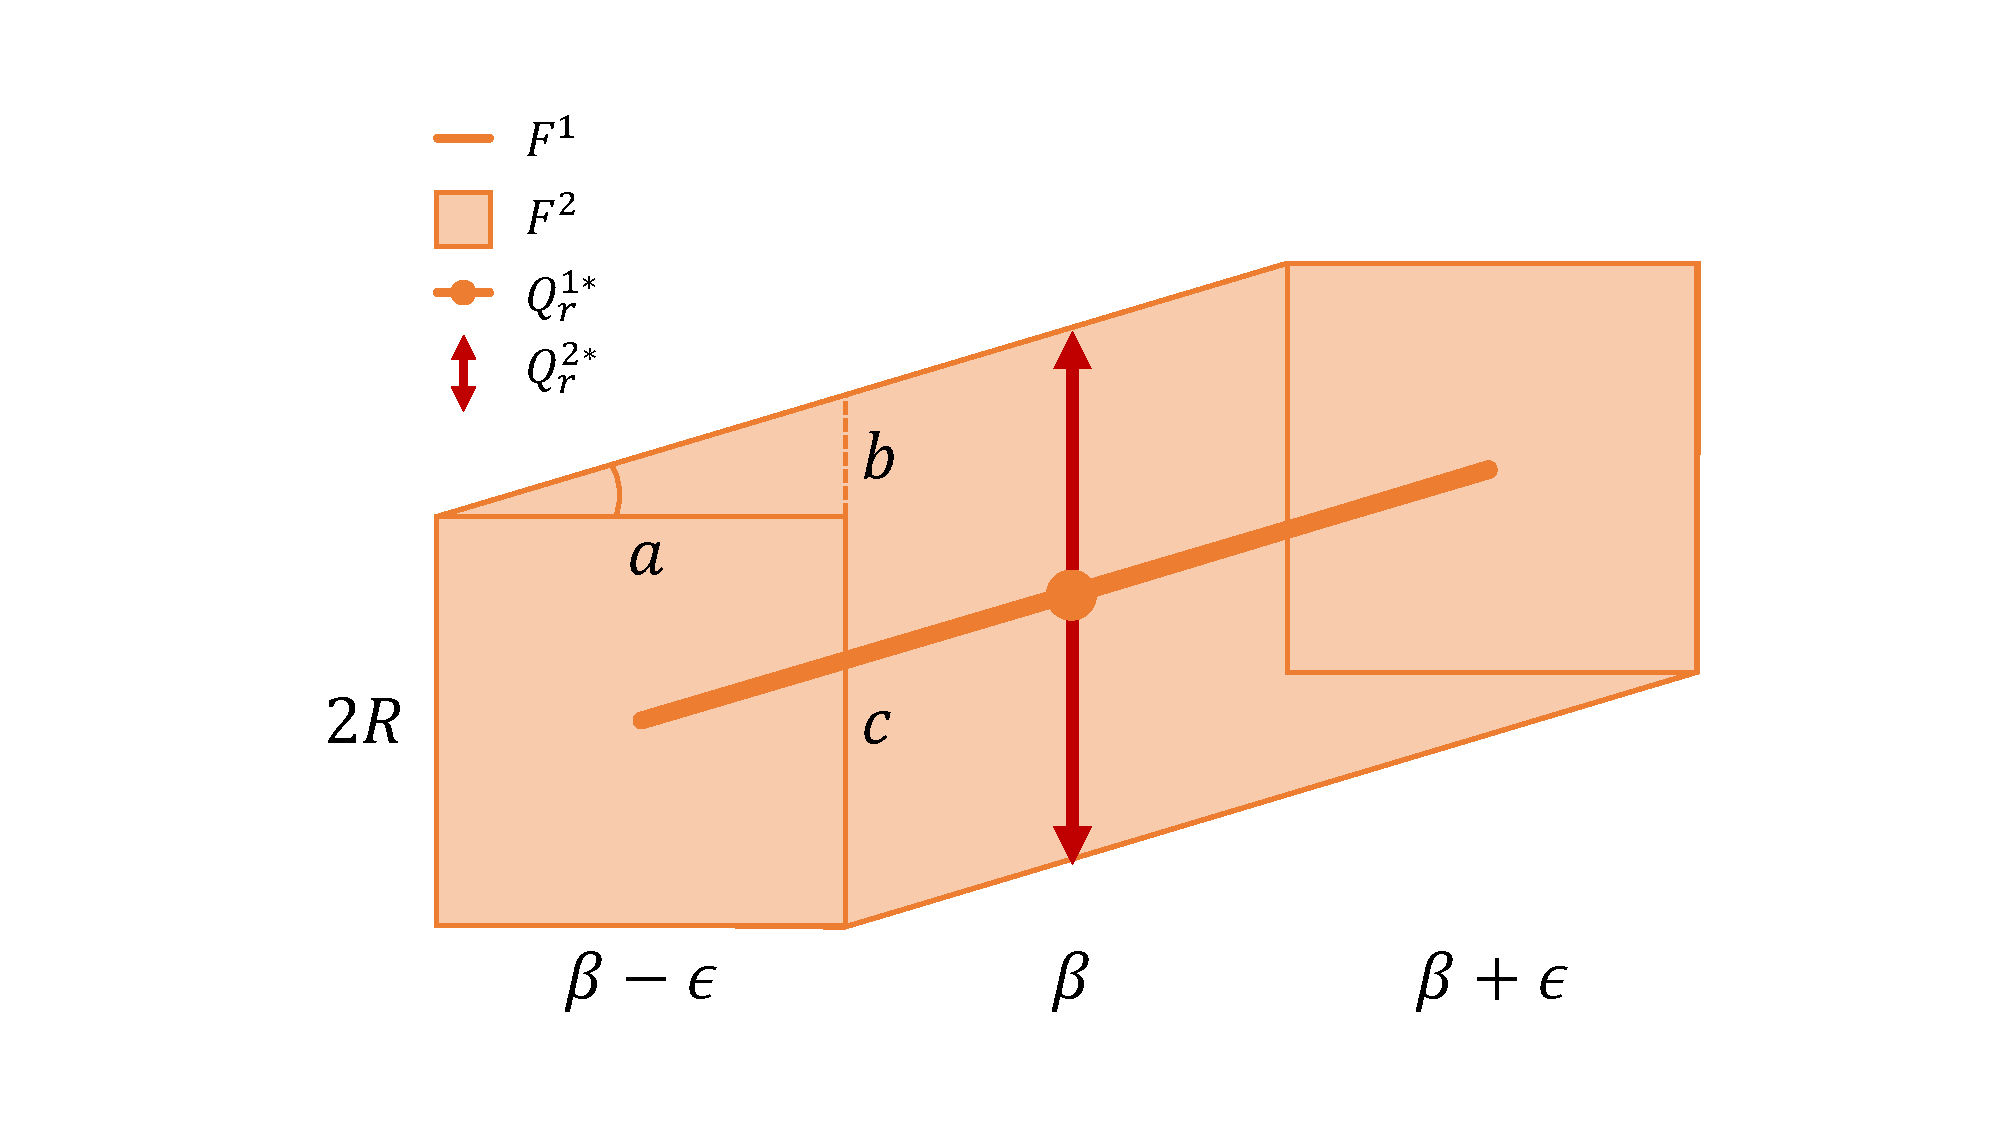
\includegraphics[trim=2cm 1cm 2cm 1cm, clip, width=0.7\textwidth]{img/contraction_lipschitz_slope.pdf}
        \caption{We represent a section $[\budget-\epsilon, \budget+\epsilon]$ of $\cF^1$ and $\text{Ball}(\cF^1, R)$. We want to bound the range of $\Qr[^{2\star}].$}
        \label{fig:contraction_lips_hull_slope}
    \end{figure}
    \begin{align*}
        \Delta \Qr[^{2\star}] &= b + c &\\
        & \leq La + c & \text{($\cF^1$ $L$-Lipschitz)}\\
        &= 2LR+2R = 2R(L+1).
    \end{align*}
    Hence,
    \begin{equation*}
        | \Qr[^{2\star}] - \Qr[^{1\star}]| \leq \frac{\Delta \Qr[^{2\star}]}{2} = R(L+1)
    \end{equation*}
    and $\Qc[^{1\star}] = \Qc[^{2\star}] = \budget$.
    Consequently, $ \|\oQ[^{2\star}] - \oQ[^{1\star}]\|_\infty \leq (L+1)R$.

    Finally, consider the edge case in \Cref{sec:proof_pi_hull}: the constraint is not active, and the optimal value is simply $\argmax_{q\in\cF} q^r$. In particular, since we showed that $\cF^2\in \text{Ball}(\cF^1, R)$, and since $\oQ[^{2\star}]\in \cF^2$, there exist $q^1\in \cF^1: \|\oQ[^{2\star}]-q^1\|_\infty\leq R$ and in particular $\oQ[^{1\star}]_r \geq q^1_r \geq \oQ[^{2\star}]_r - R$. Reciprocally, by the same reasoning, $\Qr[^{2\star}] \geq \Qr[^{1\star}] - R$. Hence, we have that $| \Qr[^{2\star}] - \Qr[^{1\star}]| \leq R \leq R(L+1).$

    \paragraph{Wrapping it up}

    We have shown that for any $\oQ^1,\oQ^2\in\cL_{\discountfactor}$,
    and all $\os\in\ocS$, $\cF^2\in\text{Ball}(\cF^1,\|\oQ^2-\oQ^1\|_\infty)$ and $\cF^1$ is
    the graph of a $L$-Lipschitz function with $L<1/\discountfactor - 1$.
    Moreover, the solutions of $\budgetedpolicy_\text{greedy}(\oQ^1)$ and $\budgetedpolicy_\text{greedy}(\oQ^2)$ at
    $\os$ are such that $ \|\oQ[^{2\star}] - \oQ[^{1\star}]\|_\infty \leq (L+1)\|\oQ^2-\oQ^1\|_\infty$.

    Hence, for all $\oa$,
    \begin{align*}
        \|\abo^{\star}\oQ^1(\os, \oa) - &\abo^{\star}\oQ^2(\os, \oa)\|_\infty \\
        &= \discountfactor\left\|\expectedvalueover{\os'\sim\augmentedtransition(\os'|\os,\oa)}
        \expectedvalueover{\oa'\sim\budgetedpolicy_\text{greedy}(\oQ^1)}\oQ^1(\os',\oa') -
        \expectedvalueover{\oa'\sim\budgetedpolicy_\text{greedy}(\oQ^2)}\oQ^2(\os',\oa')\right\|_\infty \\
        &= \discountfactor\left\|\oQ[^{2\star}] - \oQ[^{1\star}]\right\|_\infty \\
        &\leq \discountfactor(L+1)\|\oQ^2-\oQ^1\|_\infty.
    \end{align*}
    Taking the sup on $\ocS\ocA$,
    \begin{equation*}
        \|\abo^{\star}\oQ^1 - \abo^{\star}\oQ^2\|_\infty \leq \discountfactor(L+1)\|\oQ^1-\oQ^2\|_\infty
    \end{equation*}
    with $\discountfactor(L+1) < 1$.
    As a conclusion, $\abo^{\star}$ is a $\discountfactor(L+1)$-contraction on $\cL_{\discountfactor}$.
\end{proof}

%\subsection{\Cref{lemma:concavity}}

%\begin{proof}. Let $s,s'\in\cS, a\in\cA$.
%We first prove those results for $V_r^{\star}(s', \cdot)$

%\textbf{Non-decreasing}

%Consider $\beta_a^1 \leq \beta_a^2 \in \cB$.
%Any policy that satisfies the budget $\beta_a^1$ in $s'$ also satisfies $\beta_a^2$, so $\Pi_c(s', \beta_a^1) \subset \Pi_c(s', \beta_a^2)$. Hence, by taking the max over policies, $V_r^{\star}(s', \beta_a^1) \leq V_r^{\star}(s', \beta_a^2)$.
%Hence, $V_r^{\star}(s', \cdot)$ is non-decreasing.

%\textbf{Concave}

%By contradiction: assume that $V_r^{\star}(s', \cdot)$ is not concave, \ie there exist $\beta^1 < \beta^2\in \cB$ and $p\in(0, 1)$ such that $\beta^3 = (1-p)\beta^1 + p\beta^2$ verifies: $V_r^{\star}(s', \beta^3) < (1-p)V_r^{\star}(s', \beta^1) + pV_r^{\star}(s',\beta^2)$. By definition of $V^{\star}$, there must be $\pi_1,\pi_2\in\Pi^{\star}$ such that $V^{\star}(s', \beta^1) = V^{\pi_1}(s', \beta^1)$ and $V^{\star}(s', \beta^2) = V^{\pi_2}(s', \beta^2)$. 

%Define $\pi = (1-p)(\pi_1(\cdot, \beta^1), \pi_1) + p(\pi_2(\cdot, \beta^2), \pi_2)$. By linearity of $V^\pi$ with respect to $\pi$, we have that $V_c^\pi(s', \beta^3) = (1-p)V_c^{\pi_1}(s', \beta^1) + pV_c^{\pi_2}(s', \beta^2) \leq (1-p)\beta^1 + p\beta^2 = \beta^3$ since $\pi_1, \pi_2\in\Pi^{\star}(s')\subset\Pi_a(s')$, so $\pi$ respects the budget $\beta^3$. Moreover, we also have $V_r^\pi(s', \beta^3) = (1-p)V_r^{\pi_1}(s', \beta^1) + pV_r^{\pi_2}(s', \beta^2) > V_r^{\star}(s', \beta^3)$, which contradicts the definition of $V_r^{\star}$.

%Consequently, $V_r^{\star}(s', \cdot)$ is non-decreasing and concave. By \eqref{eq:bellman_expectation_Q} we see that $Q_r^{\star}(s,a,\cdot) = R_r(s,a) + \discount\expectedvalueover{s'}V_r^{\star}(s', \cdot)$  is too.


%\end{proof}

%\subsection{\Cref{lemma:tau_concavity}}


%\subsection{\Cref{lemma:pi_hull}}

%\td

%\begin{proof}
%If the estimates $q^c_0, q^c_1$ are accurate, then by construction and linearity of the expectation, the returned mixture policy has an expected total cost of $\expectedvalueover{a, \beta_a \sim\pi_\text{greedy}}Q_c(s, a, \beta_a) = \beta$ as desired in \eqref{eq:pi_greedy_constraint}. Because the $Q_r(s,a,\cdot)$ is concave and under its tangents, this mixture must have the largest $Q_r$ possible as required in \eqref{eq:pi_greedy_reward}. The special case of a tie $q_r^0 = q_r^1$ is considered, where we do minimise $Q_c$ as required in \eqref{eq:pi_greedy_cost}.
%\end{proof}


\subsection{Proof of \Cref{prop:bftq_pi_hull}}
\label{sec:proof_pi_hull}
\begin{definition}
	\begin{leftbar}[defnbar]
	Let $A$ be a set, and $f$ a function defined on $A$. We define
	
	\begin{itemize}
		\item the convex hull of $A$: $\cC(A) = \{\sum_{i=1}^p \lambda_i a_i: a_i\in A, \lambda_i\in\Real^+, \sum_{i=1}^p \lambda_i = 1, p\in\Natural\}$;
		\item the convex edges of $A$: $\cC^2(A) = \{\lambda a_1 + (1-\lambda)a_2: a_1, a_2\in A, \lambda\in[0, 1]\}$;
		\item Dirac distributions of $A$: $\dirac(A) = \{\dirac(a-a_0): a_0\in A\}$;
		\item the image of $A$ by $f$: $f(A) = \{f(a): a\in A\}$.
	\end{itemize}
\end{leftbar}
\end{definition}

\begin{proof}
Let $\os=(s,\budget)\in\ocS$ and $\oQ\in(\Real^2)^{\ocS\ocA}$. We recall the definition of $\budgetedpolicy_\text{greedy}$:
    \begin{subequations}
        \begin{align}
            \budgetedpolicy_\text{greedy}(\oa|\os; \oQ) &\in \argmin_{\rho\in\policies_r^{\oQ}} \expectedvalueover{\oa\sim\rho}\Qc(\os, \oa) \tag{\ref{eq:pi_greedy_cost}}\\
            \text{where }\quad\policies_r^{\oQ} = &\argmax_{\rho\in\cM(\ocA)} \expectedvalueover{\oa\sim\rho} \Qr(\os, \oa) \tag{\ref{eq:pi_greedy_reward}}\\
            & \text{ s.t. }  \expectedvalueover{\oa\sim\rho} \Qc(\os, \oa) \leq \budget \tag{\ref{eq:pi_greedy_constraint}}
        \end{align}
    \end{subequations}

    Note that any policy in the $\argmin$ in \eqref{eq:pi_greedy_cost} is suitable to compute $\abo^{\star}$.
    We first reduce the set of candidate optimal policies.
    Consider the problem described in \eqref{eq:pi_greedy_reward},\eqref{eq:pi_greedy_constraint}: it can be seen as a single-step \gls{CMDP} problem with reward $\reward=\Qr$ and cost $\constraint=\Qc$. By \citep[Theorem 4.4][]{Beutler1985}, we know that the solutions are mixtures of two deterministic policies. Hence, we can replace $\cM(\cA)$ by $\cC^2(\dirac(\ocA))$ in \eqref{eq:pi_greedy_reward}.

    Moreover, remark that:
    \begin{align*}
        \{\expectedvalueover{\oa\sim\rho} \oQ(\os,\oa):& \rho\in \cC^2(\dirac(\ocA))\} \\
        &= \{\expectedvalueover{\oa\sim\rho} \oQ(\os,\oa): \rho=(1-\lambda)\dirac(\oa-\oa_1)+\lambda\dirac(\oa-\oa_2), \oa_1,\oa_2\in\ocA, \lambda\in[0,1]\} \\
        &= \{(1-\lambda)\oQ(\os, \oa_1)+\lambda \oQ(\os, \oa_2), \oa_1,\oa_2\in\ocA, \lambda\in[0,1]\} \\
        &= \cC^2(\oQ(\os,\ocA))\}.
    \end{align*}

    Hence, the problem \eqref{eq:pi_greedy_reward}, \eqref{eq:pi_greedy_constraint} has become:
    \begin{equation*}
        \tilde{\policies}^{\Qr} = \argmax_{(q_r, q_c)\in\cC^2(\oQ(\os, \ocA))} q_r \quad\text{ s.t. }\quad q_c \leq \budget
    \end{equation*}
    and the solution of $\budgetedpolicy_\text{greedy}$ is $q^{\star}=\argmin_{q\in\tilde{\policies}^{\Qr}} q_c$.

    The original problem in the space of actions $\ocA$ is now expressed in the space of values $\oQ(\os, \ocA)$ (which is why we use $=$ instead of $\in$ before $\argmin$ here).

    We further restrict the search space of $q^{\star}$ following two observations:
    \begin{enumerate}
        \item $q^{\star}$ belongs to the \emph{undominated} points $\cC^2(\oQ^-)$:
        \begin{align}
            \label{eq:q_minus_undominated}
            \oQ^+ &= \{(q_c, q_r): q_c > q_c^{\pm} = \min_{q^+} q_c^+\text{ s.t. }q^+\in\argmax_{q\in \oQ(\os,\ocA)} q_r\}\\
            \oQ^- &= \oQ(\os,\ocA) \setminus \oQ^+.
        \end{align}
        Denote $q^{\star}$ = $(1-\lambda) q^1 + \lambda q^2$, with $q^1, q^2\in \oQ(\os,\ocA)$. There are three possible cases:
        \begin{enumerate}
            \item $q^1, q^2 \not\in \oQ^-$. Then $q_c^{\star} = (1-\lambda) q^1_c + \lambda q^2_c > q_c^{\pm}$. But then $q_c^{\pm} < q_c^{\star} \leq \budget$ so $q^{\pm}\in\tilde{\policies}^{\Qr}$ with a strictly lower $q_c$ than $q^{\star}$, which contradicts the $\argmin$.
            \item $q^1\in \oQ^-, q^2 \not\in \oQ^-$. But then consider the mixture $q^\top = (1-\lambda) q^1 + \lambda q^\pm$. Since $q_r^{\pm} \geq q_r^{2}$ and $q_r^{\pm} < q_r^{2}$, we also have $q^\top_r \geq q_r^{\star}$ and $q^\top_c < q_c^{\star}$, which also contradicts the $\argmin$.
            \item $q^1,q^2\in \oQ^-$ is the only remaining possibility.
        \end{enumerate}
        \item $q^{\star}$ belongs to the \emph{top frontier} $\cF$:
        \begin{equation}
            \label{eq:top-frontier}
            \cF_{\oQ} = \{q\in \cC^2(\oQ^-): \not\exists q'\in \cC^2(\oQ^-): q_c=q_c'\text{ and }q_r<q_r'\}.
        \end{equation}
        Trivially, otherwise q' would be a better candidate than $q^{\star}$.
    \end{enumerate}


    Let us characterise this frontier $\cF$. It is both:
    \begin{enumerate}
        \item the \emph{graph of a non-decreasing function}: $\forall q^1, q^2\in\cF$ such that $q_c^1\leq q_c^2$ then $q_r^1\leq q_r^2$.\\
        By contradiction, if we had $q_r^1 > q_r^2$, we could define $q^\top = (1-\lambda)q^1 + \lambda q^\pm$ where $q^\pm$ is the dominant point as defined in \eqref{eq:q_minus_undominated}. By choosing $\lambda=(q^2_c-q^1_c)/(q^\pm_c-q^1_c)$ such that $q^\top_c = q_c^2$, then since $q_r^\pm \geq q_r^1 > q_r 2$ we also have $q^\top_r > q_r^2$ which contradicts $q^2\in\cF$.
        \item the \emph{graph of a concave function}: $\forall q^1, q^2, q^3\in\cF$ such that $q_c^1\leq q_c^2 \leq q_c^3$ with $\lambda$ such that $q^2_c = (1-\lambda)q^1_c + \lambda q^3_c$, then $q_r^2 \geq (1-\lambda)q_r^1 + \lambda q_r^3$.\\
        Trivially, otherwise the point $q^\top = (1-\lambda)q^1 + \lambda q^3$ would verify $q^\top_c=q^2_c$ and $q^\top_r > q^2_r$, which would contradict $q^2 \in\cF$.
    \end{enumerate}

    We denote $\cF_{\oQ} = \cF \cap \oQ$. Clearly, $q^{\star}\in\cC^2(\cF_{\oQ})$: let $q^1, q^2\in \oQ^-$ such that $q^{\star} = (1-\lambda)q^1 + \lambda q^2$. First, $q^1, q^2\in \oQ^-\subset\cC^2(\oQ^-)$. Then, by contradiction, if there existed $q^{1'}$ or $q^{2'}$ with equal $q_c$ and strictly higher $q_r$, again we could build an admissible mixture $q^{\top}=(1-\lambda)q^{1'}  + \lambda q^{2'}$ strictly better than $q^{\star}$.

    $q^{\star}$ can be written as $q^{\star} = (1-\lambda)q^1 + \lambda q^2$ with $q^1, q^2\in\cF_{\oQ}$ and, without loss of generality, $q^1_c \leq q^2_c$.

    \paragraph{Regular case}

    There exists $q^0\in\cF_{\oQ}$ such that $q^0_c \geq \budget$. Then $q^1$ and $q^2$ must flank the budget: $q_c^1 \leq \budget \leq q_c^2$. Indeed, by contradiction, if $q_c^2 \geq q_c^1 > \budget$ then $q_c^{\star} > \budget$ which contradicts $\policies_r^{\oQ}$. Conversely, if $q_c^1 \leq q_c^2 < \budget$ then $q^{\star} < \budget \leq q^0_c$, which would make $q^{\star}$ a worse candidate than $q^\top=(1-\lambda)q^{\star} + \lambda q^0$ when $\lambda$ is chosen such that $q_c^\top=\budget$, and contradict $\policies_r^{\oQ}$ again.

    Because $\cF$ is the graph of a non-decreasing function, $\lambda$ should be as high as possible, as long as the budget $q^{\star}\leq\budget$ is respected. We reach the highest $q_r^{\star}$ when $q^{\star}_c=\budget$, that is: $\lambda=(\budget-q_c^1)/(q_c^2-q_c^1)$.

    It remains to show that $q^1$ and $q^2$ are two successive points in $\cF_{\oQ}$: $\not\exists q\in\cF_{\oQ}\setminus\{q^1, q^2\}: q^1_c \leq q_c \leq q^2_c$. Otherwise, as $\cF$ is the graph of a concave function, we would have $q_r \geq (1-\mu)q_r^1 + \mu q_r^2$. $q_r$ cannot be strictly greater than $(1-\mu)q_r^1 + \mu q_r^2$ which would contradict $q^{\star}$, but it can still be equal, which means the tree points $q, q^1, q^2$ are aligned. In fact, every points aligned with $q^1$ and $q^2$ can also be used to construct mixtures resulting in $q^{\star}$, but among these solutions we can still choose $q^1$ and $q^2$ as the two points in $\cF_{\oQ}$ closest to $q^{\star}$.

    \paragraph{Edge case}

    $\forall q\in\cF_{\oQ}, q_c < \budget$. Then  $q^{\star} =  \argmax_{q\in\cF} q_r = q^\pm =  \argmax_{q\in \oQ^-} q_r$.
\end{proof}


%\begin{proof}
%First, a straightforward proof by induction shows that for all $k\in\Natural$, $Q_k$ computed at iteration $k$ of either \Cref{alg:bvi} or \Cref{alg:bftq} is concave non-decreasing with respect to $\beta_a$: the initialisation is trivial from $Q_0 = 0$, and the heredity stems from \Cref{lemma:tau_concavity}.
%\end{proof}


% \subsection{Decomposition Lemma}

% \begin{lemma}
%     For any sequence real valued functions $f_1,\ldots,f_n$ and any real number $c$, we have
%     \[
%         \begin{array}{lcl}
%             \underbrace{\max\limits_{\sum_i x_i \leq c}\sum_j f_j(x_j)}_{(a)} & \quad{}=\quad{} & \underbrace{\max\limits_{\sum_i c_i \leq c}\left(\sum_j\max\limits_{x\leq c_j} f_j(x)\right)}_{(b)}\\
%         \end{array}
%     \]
% \end{lemma}

% \begin{proof}
%     Let us first show that $(a)\leq(b)$.
%     By definition of the maximum on a set, for any $f_j$ and any $c_j$ we have
%     $\max\limits_{x\leq c_j} f_j(x) \geq f_j(c_j)$.
%     Hence, by replacing these terms in $(b)$ we get:
%       \[
%     \begin{array}{lcl}
%         \max\limits_{\sum_i c_i \leq c} \sum_j f_j(c_j) & \quad{}\leq\quad{} & \max\limits_{\sum_i c_i\leq c}\left(\sum_j \max\limits_{x_j\leq c_j} f_j(x_j)\right)\\
%     \end{array}
%     \]
%     The left hand side of this inequality is just a rewriting of $(a)$ with different dummy variables names.

%     Let us show now that $(a) \geq (b)$.
%     Let $\hat{x}_1,\ldots,\hat{x}_n, \hat{c}_1, \ldots \hat{c}_n$ be a realisation (argmax) of $(b)$.
%     By definition of $(b)$'s feasible set, we have $\sum_i\hat{c}_i \leq c$ and for any $i$: $\hat{x}_i\leq \hat{c}_i$.
%     Because $\sum_i\hat{x}_i\leq \sum_i\hat{c}_i \leq c$, the tuple $(\hat{x}_1, \ldots \hat{x}_n)$ is also a feasible value for $(a)$. And, by definition of the maximum on a set: $(a) = \max\limits_{\sum_i x_i \leq c} \sum_j f_j(x_j) \geq \sum_j f_j(\hat{x}_j) = (b)$.
% \end{proof}

%\section{Risk-Sensitive Exploration}
%\label{sec:risk-sensitive-supp}
%We recall the Risk-Sensitive Exploration in %\Cref{alg:risk-sensitive-exploration}:
%\begin{algorithm}[ht]
\DontPrintSemicolon
\KwData{An environment, a BFTQ solver, $W$ CPU workers}
\KwResult{A batch of transitions $\cD$}
$\cD\leftarrow\emptyset$\;
\For{each intermediate batch} {
split episodes between $W$ workers\;
\For(\tcp*[f]{run this loop on each worker in parallel}){each episode in batch}{
sample initial budget $\beta\sim\mathcal{U}(\mathcal{B})$.\;
\While{episode not done}{
update $\epsilon$ from schedule.\;
sample $z\sim\mathcal{U}([0, 1])$.\;
\lIf{$z < \epsilon$}{sample $(a, \beta_a)\sim\mathcal{U}(\Delta_{\cA\cB})$.\tcp*[f]{Explore}}
\lElse{sample $(a, \beta_a)\sim\pi_\text{greedy}(a, \beta_a|s, \beta; Q^{\star})$.\tcp*[f]{Exploit}}
append transition $(s, \beta, a, \beta_a, R, C, s')$ to batch $\mathcal{D}$.\;
step episode budget $\beta \leftarrow \beta_a$
}
}
$\pi_\text{greedy}(\cdot\sim; ~Q^{\star}) \leftarrow\texttt{BFTQ}(\cD)$.
}
\Return{the batch of transitions $\cD$}
\caption{Risk-sensitive exploration}
\label{algo:risk-sensitive-exploration}
\end{algorithm}

	%!TEX root = ../../PhD_thesis__Edouard_Leurent.tex
\graphicspath{{2-Chapters/6-Chapter/}}

\chapter{Complements on \Cref{chapter:6}}

\paragraph{Outline}
We provide proofs for every claimed result in \Cref{sec:kl-olop-proofs}.
We look into the time and memory complexity and propose efficient implementations of \OLOP and \KLOLOP in \Cref{sec:kl-olop-time}, and of \GBOPD and \GBOP in \Cref{sec:gbop-implementation}.

\section{Proofs}
\label{sec:kl-olop-proofs}

\subsection{Proof of \Cref{lemma:expected-regret}}
\label{sec:proof-lem-expected-regret}
\begin{proof}
	The proof is identical to that of Lemma 4 in \citep{Bubeck2010}.
	
	Since $\arg \max _{a \in \cA} T_{a}(M)$, and $\sum_{a \in \cA} T_{a}(M)=M,$ we have $T_{a(n)}(M) \geq M / K$, and thus:
	\begin{equation*}
	\frac{M}{K}(V-V(a(n))) \leq(V-V(a(n))) T_{a(n)}(M) \leq \sum_{m=1}^{M} V-V\left(a^{m}\right)
	\end{equation*}
	Hence, we have, $r_{n} \leq \frac{K}{M} \sum_{m=1}^{M} V-V\left(a^{m}\right)$. Now remark that, for any sequence of actions $a\in \cA^L$, we have either:
	\begin{itemize}
		\item $a_{1 : H} \in \mathcal{I}_{H} ;$ which implies $V-V(a) \leq \frac{2 \gamma^{H+1}}{1-\gamma}$
		\item or there exists $1\leq h \leq H$ such that $a_{1:h} \in \mathcal{J}_h$; which implies $V-V(a) \leq V-V\left(a_{1 : h-1}\right)+\frac{\gamma^{h}}{1-\gamma} \leq \frac{3 \gamma^{h}}{1-\gamma}$.
	\end{itemize}
	Thus we can write:
	\begin{equation*}
	\begin{aligned} \sum_{m=1}^{M}\left(V-V\left(a^{m}\right)\right) &=\sum_{m=1}^{M}\left(V-V\left(a^{m}\right)\right)\left(\mathbbm{1}\left\{a^{m} \in \mathcal{I}_{H}\right\}+\mathbbm{1}\left\{\exists 1 \leq h \leq H : a_{1 : h}^{m} \in \mathcal{J}_{h}\right\}\right) \\ & \leq \frac{2 \gamma^{H+1}}{1-\gamma} M+3 \sum_{h=1}^{H} \sum_{a \in \mathcal{J}_{h}} \frac{\gamma^{h}}{1-\gamma} T_{a}(M) \end{aligned}
	\end{equation*}
	
\end{proof}

\subsection{Proof of \Cref{lemma:size_Ph}}
\label{sec:proof-size_Ph}
\begin{proof}
	The event $\tau^a_{h,h'}=1$ implies $a^{m+1}\in a A^*$ and \eqref{eq:sampled-enough}. This implies by \Cref{lemma:sub-optimal-pull} that either \eqref{eq:cond-ukl}, \eqref{eq:cond-lkl} or \eqref{eq:cond-dkl} is satisfied. Now by \Cref{lemma:ci-length} this implies that either \eqref{eq:cond-ukl} is true or \eqref{eq:cond-lkl} is true or \eqref{eq:sampled-enough-h} is false. We now prove that if \eqref{eq:P-min-size} is not satisfied then \eqref{eq:sampled-enough} is true, which clearly ends the proof.
	This follows from: For any $0 \leq t \leq h'$:
	
	\begin{align*}
	T_{a_{1:t}}(m) &= \sum_{b\in a_{1:t}A^{h-t}} T_b(m) \geq \sum_{b\in \mathcal{P}^{a_{1:t}}_{h,h'}} T_b(m) \\
	&\geq \left(\gamma^{2(t-h')}\right) \left(2f(m)(h+1)^2\gamma^{2(h'-h-1)}\right)\\
	&= 2f(m)(h+1)^2\gamma^{2(t-h-1)}\,.\qquad\qquad
	\end{align*}
	%\
\end{proof}

\subsection{Proof of \Cref{lemma:expected-P-size}}
\label{sec:proof-expected_P_size}
\begin{proof}
	The proof is identical to that of Lemma 9 in \citep{Bubeck2010}.
	
	\noindent
	Let $h'\geq 1$ and $0 \leq s \leq h'$. We introduce the following random variables:
	\begin{equation*}
	m_{s}^{a}=\min \left(M, \min \left\{m \geq 0 :\left|\mathcal{P}_{h, h^{\prime}}^{a}(m)\right| \geq \gamma^{2\left(s-h^{\prime}\right)}\right\}\right).
	\end{equation*}
	We will prove recursively that,
	\begin{equation}
	\label{eq:toprove}
	\left|\mathcal{P}_{h, h^{\prime}}^{\emptyset}(m)\right| \leq \sum_{t=0}^{s} \gamma^{2\left(t-h^{\prime}\right)}\left|\mathcal{I}_{t}\right|+\sum_{a \in \mathcal{I}_{s}}\left|\mathcal{P}_{h, h^{\prime}}^{a} \setminus \cup_{t=0}^{s} \mathcal{P}_{h, h^{\prime}}^{a_{1:t}}\left(m_{t}^{a_{1:t}}\right)\right|
	\end{equation}
	The result is true for $s = 0$ since $\mathcal{I}_0 = \{\emptyset\}$ and by definition of $m^\emptyset_0$,
	\begin{equation*}
	\left|\mathcal{P}_{h, h^{\prime}}^{\emptyset}(m)\right| \leq \gamma^{-2 h^{\prime}}+\left|\mathcal{P}_{h, h^{\prime}}^{\emptyset}(m) \setminus \mathcal{P}_{h, h^{\prime}}^{\emptyset}\left(m_{0}^{\emptyset}\right)\right|
	\end{equation*}
	Now let us assume that the result is true for $s<h'$. We have:
	\begin{align*}
	\sum_{a \in \mathcal{I}_{s}}\left|\mathcal{P}_{h, h^{\prime}}^{a}(m) \setminus \cup_{h, h^{\prime}}^{a_{1 : t}}\left(m_{t}^{a_{1 : t}}\right)\right|&=\sum_{a \in \mathcal{I}_{s+1}}\left|\mathcal{P}_{h, h^{\prime}}^{a}(m) \setminus \cup_{t=0}^{s} \mathcal{P}_{h, h^{\prime}}^{a_{1 : t}}\left(m_{t}^{a_{1 : t}}\right)\right|\\
	&\leq \sum_{a \in \mathcal{I}_{s+1}} \gamma^{2\left(s+1-h^{\prime}\right)}+\left|\mathcal{P}_{h, h^{\prime}}^{a}(m) \setminus \cup_{t=0}^{s+1} \mathcal{P}_{h, h^{\prime}}^{a_{1 : t}}\left(m_{t}^{a_{1 : t}}\right)\right|\\
	&= \gamma^{2\left(s+1-h^{\prime}\right)}\left|\mathcal{I}_{s+1}\right|+\sum_{a \in \mathcal{I}_{s+1}}\left|\mathcal{P}_{h, h^{\prime}}^{a}(m) \setminus \cup_{t=0}^{s+1} \mathcal{P}_{h, h^{\prime}}^{a_{1 ; t}}\left(m_{t}^{a_{1 : t}}\right)\right|
	\end{align*}
	which ends the proof of \eqref{eq:toprove}. Thus we proved (by taking $s=h'$ and $m=M$):
	\begin{equation*}
	\begin{aligned}\left|\mathcal{P}_{h, h^{\prime}}^{\emptyset}(M)\right| & \leq \sum_{t=0}^{h^{\prime}} \gamma^{2\left(t-h^{\prime}\right)}\left|\mathcal{I}_{t}\right|+\sum_{a \in \mathcal{I}_{h^{\prime}}}\left|\mathcal{P}_{h, h^{\prime}}^{a}(M) \setminus \cup_{t=0}^{s+1} \mathcal{P}_{h, h^{\prime}}^{a_{1 : t}}\left(m_{t}^{a_{1 : t}}\right)\right.\\ &=\sum_{t=0}^{h^{\prime}} \gamma^{2\left(t-h^{\prime}\right)}\left|\mathcal{I}_{t}\right|+\sum_{a \in \mathcal{J}_{h}}\left|\mathcal{P}_{h, h^{\prime}}^{a}(M) \setminus \cup_{h, h^{\prime}}^{a_{1 : t}}\left(m_{t}^{a_{1 : t}}\right)\right| \end{aligned}
	\end{equation*}
	
	Now, for any $a\in \mathcal{J}_h$, let $\tilde{m} = \max_{0\leq t\leq h'} m_t^{a_{1:t}}$. Note that for $m\geq \tilde{m}$, equation \eqref{eq:P-min-size} is not satisfied. Thus we have
	\begin{equation*}
	\begin{aligned}
	\left|\mathcal{P}_{h, h^{\prime}}^{a} \setminus \cup_{h, h^{\prime}}^{s+1} \mathcal{P}_{h, h^{\prime}}^{a_{1 : t}}\left(m_{t}^{a_{1 : t}}\right)\right|=&\sum_{m=\tilde{m}}^{M-1} \tau_{h, h^{\prime}}^{a}(m+1)=\sum_{m=0}^{M-1} \tau_{h, h^{\prime}}^{a}(m+1) \mathbbm{1}\{\eqref{eq:P-min-size} \text { is not satisfied }\} \\ & \leq \sum_{m=0}^{M-1} \tau_{h, h^{\prime}}^{a}(m+1) \mathbbm{1}\{\eqref{eq:cond-ukl} \text { or }\eqref{eq:cond-lkl}\} \end{aligned}
	\end{equation*}
	where the last inequality results from \Cref{lemma:size_Ph}. Hence, we proved:
	
	\begin{equation*}
	\left|\mathcal{P}_{h, h^{\prime}}^{\emptyset}\right| \leq \sum_{t=0}^{h^{\prime}} \gamma^{2\left(t-h^{\prime}\right)}\left|\mathcal{I}_{t}\right|+\sum_{m=0}^{M-1} \sum_{a \in \mathcal{J}_{h}} \mathbbm{1}\{\eqref{eq:cond-ukl}\text{ or }\eqref{eq:cond-lkl}\}
	\end{equation*}
	
	Taking the expectation and applying \Cref{lemma:boundary-crossing-prob} yield the claimed bound for $h'\geq 1$.
	
	Now for $h' = 0$ we need a modified version of \Cref{lemma:size_Ph}. Indeed in this case one can directly prove that $\tau_{h,0}^a(m+1)=1$ implies that either equation \eqref{eq:cond-ukl} or \eqref{eq:cond-lkl} is satisfied (this follows from the fact that $\tau_{h,0}^a(m+1)=1$ always imply that \eqref{eq:sampled-enough-h} is true for $h'= 0$). Thus we obtain:
	\begin{equation*}
	\left|\mathcal{P}_{h, h^{\prime}}^{\emptyset}\right|=\sum_{m=0}^{M-1} \sum_{a \in \mathcal{J}_{h}} \tau_{h, 0}^{a}(m+1) \leq \sum_{m=0}^{M-1} \sum_{a \in \mathcal{J}_{h}} \mathbbm{1}\{\eqref{eq:cond-ukl}\text{ or }\eqref{eq:cond-lkl}\}
	\end{equation*}
	Taking the expectation and applying \Cref{lemma:boundary-crossing-prob} yield the claimed bound for $h' = 0$ and ends the proof.
	
\end{proof}

\subsection{Proof of \Cref{lemma:expected-plays-count}}
\label{sec:proof-expected-plays-count}
\begin{proof}
	The proof is identical to that of Lemma 10 in \citep{Bubeck2010}:
	\begin{align*}
	\sum_{a \in \mathcal{J}_{h}} T_{a}(M) = {} & \sum_{a \in \mathcal{J}_{h} \backslash \mathcal{P}_{h, h-1}^{\emptyset}} T_{a}(M)+\sum_{h^{\prime}=1}^{h-1} \sum_{a \in \mathcal{P}_{h, h^{\prime}}^{\emptyset} \setminus \mathcal{P}_{h, h^{\prime}-1}^{\emptyset}} T_{a}(M)+\sum_{a \in \mathcal{P}_{h, 0}^{\emptyset}} T_{a}(M)\\
	\leq {} & 2f(m)(h+1)^{2} \gamma^{2(h-2-h)}\left|\mathcal{J}_{h}\right| \\
	 &+ \sum_{h^{\prime}=1}^{h-1} 2f(m)(h+1)^{2} \gamma^{2\left(h^{\prime}-2-h\right)} \log M\left|\mathcal{P}_{h, h^{\prime}}^{\emptyset}\right|+M\left|\mathcal{P}_{h, 0}^{\emptyset}\right|\\
	= {} &\tilde{\cO}\left(\left(\kappa^{\prime}\right)^{h}+\gamma^{-2 h} \sum_{h^{\prime}=1}^{h-1} \gamma^{2 h^{\prime}}\left|\mathcal{P}_{h, h^{\prime}}^{\emptyset}\right|+M\left|\mathcal{P}_{h, 0}^{\emptyset}\right|\right)
	\end{align*}
	Taking the expectation and applying the bound of \Cref{lemma:expected-P-size} give the claimed bound.
	
\end{proof}


%\section{Proof of \GBOP results}
%\label{sec:gbop-proofs}

\subsection{Proof of \Cref{lem:properties-b-tree}}
\label{sec:proof-properties-b-tree}
\begin{proof}
The tightening property is directly obtained by definition of monotonicity.
Let us show the preservation of monotonicity. Let $U$ a monotonic upper-bound, $a\in \cA^h$. Then, for any $b\in \cA$:
\begin{align*}
U(ab) \geq B(U)(ab) \implies 
r(ab) + \gamma U(ab) \geq r(ab) + \gamma B(U)(ab).
\end{align*}
Thus, my taking the $\max$ on $b$,
$
B(U)(a) \geq B^2(U)(a).
$
The same can be obtained for a lower-bound $L$.

The finite time convergence can be obtained by recursion from the leaves to the root, by noticing that if the value of a set of siblings $aA$ is invariant by $B$, then the value of their parent $a$ is invariant by $B^2$.
\end{proof}

\subsection{Proof of \Cref{lem:properties-b-graph}}
\label{sec:proof-properties-b-graph}
\begin{proof}
The proof of tightening and monotonicity preservation is the same as that of \Cref{lem:properties-b-tree}.
The contraction property is standard for the Bellman Operator, see \eg Puterman M., Markov Decision Processes: Discrete Stochastic Dynamic Programming (2005).
\end{proof}

\subsection{Proof of \Cref{lem:sequence-values}}
\label{sec:proof-sequence-values}
\begin{proof}
By definition, for $a\in\cA^h$,
\begin{align*}
V(a) &= \sup_{b\in a\cA^\infty} \sum_{t=1}^\infty \discount^t\mu(b_{1:t}) \\
     &= \sum_{t=1}^h \discount^t\mu(a_{1:t})  \sup_{b\in a\cA^\infty} \sum_{t=h+1}^\infty \discount^t\mu(b_{1:t}) \\
     &= G(s_1,a) \discount^h \sup_{b\in \cA^\infty} \sum_{t=1}^\infty \discount^t\mu(b_{1:t}\text{ starting from $s(a)$}) \\
     &= G(s_1,a) \discount^h V(s(a))
\end{align*}
\end{proof}

\subsection{Proof of \Cref{thm:regret-opd}}
\label{sec:proof-regret-opd}
We recall the main steps of the proof of \citet{Hren2008}.\\

\begin{enumerate}
	\item The recommendation $a_n$ has a maximal depth $d_n$ in the tree, and its gap $\regret = V^\star - V({a_{n,1}})$ is bounded by $\regret \leq \frac{\gamma^{d_n}}{1-\gamma}$. We need to relate $d_n$ to $n$.
	
	\item Each expanded node belongs to $\Tau^\infty = \bigcup_{h\geq 0} \Tau_h^\infty$, where $$\Tau_h^\infty = \left\{a\in \cA^h: V^\star-V(a) \leq \frac{\gamma^h}{1-\gamma}\right\}.$$ Introduce the difficulty measure $\kappa$ such that $|\Tau_h^\infty| = \cO(\kappa^h)$ (the smallest).
	
	\item In the worst case, expanded nodes fully fill the depths of $\Tau^\infty$ up to $d_n$: $n = \sum_{d=1}^{d_n} n_d \leq  C\sum_{d=1}^{d_n} \kappa^d = \begin{cases}
	\cO(d_n) &\text{if $\kappa=1$}\\
	\cO(\kappa^{d_n}) &\text{else.}
	\end{cases}$\\
	Hence $\regret = \begin{cases}
	\cO(\gamma^n) &\text{if $\kappa=1$}\\
	\cO(\gamma^{\frac{\log n}{\log \kappa}}) = \cO(n^{-\frac{\log 1/\gamma}{\log \kappa}}) &\text{else.}
	\end{cases}$
\end{enumerate}

\subsection{Proof of \Cref{lem:shrink}}
\label{sec:proof-shrink}
\begin{proof}
Let $L_2\leq L_1\leq V\leq U_1\leq U_2$, then $\Tau_h^\infty(L_1,U_1) \subset \Tau_h^\infty(L_2,U_2),$ which implies $$|\Tau_h^\infty(L_1,U_1)|^{1/h} \leq |\Tau_h^\infty(L_2,U_2)|^{1/h}$$ and the claimed result in the limit $h\rightarrow\infty$.
\end{proof}

\subsection{Proof of \Cref{thm:regret-bound-U}}
\label{sec:proof-regret-bound-U}
In this proof, we temporarily assume that $U=B(U)$ and $L=B(L)$. We follow the same steps as in the proof of the regret of \OPD.

\begin{remark}
\begin{leftbar}[remarkbar]
It no longer holds that $a_n$ must be of maximal depth $d_n$.  This is due to the fact the exploration bonus $\gamma^h U(a)$ is not depth-wise constant: consider two nodes $a,b$ at the same depth with $R(a) > R(b)$. In \OPD, both get the same bonus $\gamma^h/(1-\gamma)$, and the node $a$ is expanded first. But with the local bonus, $b$ could be expanded in priority rather than $a$, if its own bonus is sufficiently higher than that of $a$, precisely if $R(a)+\gamma^h U(a) < R(b)+\gamma^h U(b)$. For instance, $U(a)=0$ when $a$ is known to be a terminal state while $b$ can lead to future rewards. If after expanding and exploring the subtree of $b$ we find out that $V(b) = 0$, we still return the recommendation $a$, which is of non-maximal depth.
\end{leftbar}
\end{remark}

The regret bound still holds, however. First, notice that:
\begin{lemma}[Expansion]
\begin{leftbar}[lemmabar]
\label{lem:expansion-bound-U}
Whenever a node $a$ of depth $h$ is expanded by the optimistic algorithm, its first action $a_1$ enjoys a simple regret $V(a^\star)-V(a_1) \leq \gamma^h(U(a)-L(a))$. 
\end{leftbar}
\end{lemma}
\begin{proof}
Let $t$ be the time of expansion of $a$, it holds that $\overline{U}_t(b) \leq \overline{U}_t(a)$ for all $b\in \ext{\Tau}_t$, in particular those in a branch starting by an optimal action $a^\star$. Since $U=B(U)$ and $L=B(L)$, we also have $\overline{U}_t(a^\star) = \max_{b\in a^\star A^*} \overline{U}_t(b) \leq \overline{U}_t(a)$, and $\overline{L}_t(a_1) = \max{b\in a_1 A^*} \overline{L}_t(b) \geq  \overline{L}_t(a)$. Thus, $V(a^\star)-V(a_1) \leq \overline{U}_t(a^\star) - \overline{L}_t(a_1) \leq \overline{U}_t(a) - \overline{L}_t(a) = \gamma^h(U(a)-L(a))$.
\end{proof}
 
\begin{lemma}[Recommendation]
\begin{leftbar}[lemmabar]
\label{lem:recommendation-bound-U}
The recommended action $a_n$ has a simple regret $\regret \leq \frac{\gamma^{d_n}}{1-\gamma}$, where $d_n$ is the maximal depth of $\Tau_n$.
\end{leftbar}
\end{lemma}
\begin{proof}
Let $i$ a node of maximal depth $d_n$, and consider the recommended node $a_n$ at time $n$, of depth $d$. In particular, $\overline{L}_n(a_n) \geq \overline{L}_n(i)$, and since $(\overline{L}_t)_t$ is non-decreasing we also have $\overline{L}_n(i) \geq \overline{L}_t(i)$. At the time $t$ when $i$ is expanded, we have $\overline{U}_t(a_n) \leq \overline{U}_t(i)$, and since $(\overline{U}_t)_t$ is non-increasing we also have $\overline{U}_n(a_n) \leq \overline{U}_t(a_n)$. We can conclude with \Cref{lem:expansion-bound-U} applied to $a_n$: $\regret \leq \gamma^d(U(a_n)-L(a_n) = \overline{U}_n(a_n) - \overline{L}_n(a_n)  \leq \overline{U}_t(a_n) - \overline{L}_n(i) \leq \overline{U}_t(i) - \overline{L}_t(i) = \gamma^{d_n}(U(i) - L(i)$, which yields the claimed bound since $U(i) - L(i) \leq V_{\max}-0$.
\end{proof}

\begin{lemma}[Near-optimal nodes]
\begin{leftbar}[lemmabar]
\label{lem:near-optimal-nodes-U}
Every node expanded by \eqref{eq:sampling_rule} is in $$\Tau^\infty(L,U) = \bigcup_{h\geq 0} \Tau^\infty_h(L,U).$$
\end{leftbar}
\end{lemma}
\begin{proof}
Let $a$ be a node of depth $h$ expanded at round $n$, then $\overline{U}_n(a) \geq \overline{U}_n(b)$ for all $b\in\ext{\Tau}_n$. Thus, since $U = B(U)$, we have $\overline{U}(a) = \overline{B(U)}(\emptyset) = B(U)(s_1) \geq V(s_1) = V^\star$. Thus, $V^\star - V(a) \leq \overline{U}(a) - \overline{L}(a) = \gamma^h(U(a) - L(a))$.
\end{proof}

Finally, we can move on to the proof of \Cref{thm:regret-bound-U}.
Let $n_d$ be the number of expanded nodes of depth $d$, by \Cref{lem:near-optimal-nodes-U} we have $n_d \leq |\Tau^\infty_d(L,U)| \leq C\kappa(L,U)^d$. Thus, 
\[n = \sum_{d=1}^{d_n} n_d \leq C\sum_{d=0}^{d_n} \kappa(L,U)^d = C\frac{\kappa(L,U)^{d_n+1}-1}{\kappa(L,U)-1}\]
Hence, $d_n \geq C'\frac{\log n}{\log\kappa(L,U)},$ which along with \Cref{lem:expansion-bound-U} gives the claimed bound.

Note that if $L,\,U$ are monotonic bounds that do not verify $L = B(L)$ and $U=B(U)$, then planning with $B(L),B(U)$ instead will yield the proved bound with a branching factor $\kappa(B(L),B(U))$, and since $L\leq B(L)\leq V\leq B(U)\leq U$ we have $\kappa(B(L),B(U)) \leq \kappa(L,U)$, which still gives \begin{align*}
\regret = \cO\left(n^{-\frac{\log 1/\gamma}{\log \kappa(L,U)}}\right);
\end{align*}

%\section{Proof of \Cref{prop:b-eq-mb}}

%\begin{proof}
%	Let $U$ equivalent to $\cU$, and $a\in T_n$.
%	If $a\in\ext{T_n}$, then necessarily $s(a)\in\ext{\cG_n}$, and both are unchanged by $B_n$ and $\cB_n$ respectively.
%	If $a\in\inte{T_n}$, then necessarily $s(a)\in\int{\cG_n}$. There exist a'
%\end{proof}

%\section{Proof of \Cref{lem:properties-mb}}
%\begin{proof}
%Let $U_1, U_2\in \Real^\Tau_n, a\in\Tau_n$,
%\begin{align*}
%    (M_n^+ U_1 - M_n^+ U_2)(a) &= \min_{a'\in N_n(a)} U_1(a') - \min_{a'\in N_n(a)} U_2(a') \\
%    &= \min_{a'\in N_n(a)} U_1(a') - U_2(a^-) \\
%    &\leq U_1(a^-) - U_2(a^-) \\
%    &\leq \|U_1 - U_2\|_\infty
%\end{align*}
%where $a^-\in \argmin_{a'\in N_n(a)} U_2(a')$. 
%Hence, $\|M_n^+ U_1 - M_n^+ U_2\|_\infty \leq \|U_1 - U_2\|_\infty$
%\end{proof}
%
%\section{Proof of \Cref{prop:pruning}}
%
%\begin{proof}
%Assume $h(a_2) \geq h(a_1)$.
%\begin{align*}
%    V(a_1) - V(a_2) &= R(a_1)- R(a_2) + \underbrace{\left(\gamma^{h(a_1)} - \gamma^{h(a_2)}\right)}_{\geq 0}V(s) \\
%    &\leq R(a_1)- R(a_2) + \left(\gamma^{h(a_1)} - \gamma^{h(a_2)}\right)U(s)\\
%    &= \overline{U}(a_1) - \overline{U}(a_2)
%\end{align*}
%Hence, if this last term is negative, then $V(a_1) - V(a_2)$ is as well.
%\end{proof}

\subsection{Proof of \Cref{lem:equivalence}}
\label{sec:proof-equivalence}
\begin{proof}	
We first show that if $U$ is equivalent to $\cU$, meaning that for any sequence $a\in T(\cG_n)$ we have $U(a) = \cU(s(a))$, then $B_n(U)$ is equivalent to $\cB_n(\cU)$.

By definition of $T(\cG_n)$, any sequence of action $a\in T(\cG_n)$ corresponds to a path $s_1, a_1,\dots,$ $s_{h}, a_{h}, s_{h+1}$ in $\cG_n$. If $a\in\ext{T(\cG_n)}$, then necessarily $s(a)\in\ext{\cG_n}$, and both are unchanged by $B_n$ and $\cB_n$ respectively. Conversely, if $a\in\inte{T}(\cG_n)$, then $s(a)\in\inte{\cG_n}$ by construction. Thus, 
\begin{align*}
B_n(U)(a) &= \max_{b\in \cA} r(s(a), b) + \gamma U({ab}) &\\
&= \max_{b\in \cA} r(s(a), b) + \gamma \cU(s({ab})) &\text{ (by assumption)} \\
&= \max_{b\in \cA} r(s(a), b) + \gamma \cU(P(s({a}),b))\\
&= \cB_n(\cU_n)(s(a)).
\end{align*}

By induction, for any $k>0$ $B_n^k(U)$ is equivalent to $\cB_n^k(\cU)$, and at the limit $k\rightarrow\infty$ it comes that $U_n$ is equivalent to $\cU_n$. The same result can be shown similarly for $L_n$ and $\cL_n$.
\end{proof}

\subsection{Proof of \Cref{lem:expansion-bound}}
\label{sec:proof-expansion-bound}
We start by showing a preliminary lemma.
\begin{lemma}[Bounds of sequence values]
	\begin{leftbar}[lemmabar]
	\label{lem:bounds}
	The bounds $(\overline{L}_n, \overline{U}_n)$ on the value of sequences of actions verify are respectively non-decreasing and non-increasing with respect to $n$, and verify: for all $a\in \cA^*$, $\overline{U_n}(a) = \max_{a'\in a A^\infty} \overline{U}(a')$.
	\end{leftbar}
\end{lemma}
\begin{proof}
	The second property can be easily shown by induction using the fact that $U_n$ and $L_n$ are fixed-points of $B_n$ by definition. Applying this equation at each depth $h$ gives the result. From this observation, we can deduce that $\overline{L}_n$ is increasing with $n$. Indeed, since when $T(\cG_n)$ is expanded with additional nodes compared to $T(\cG_{n-1})$, the leaves $a$ of $T(\cG_{n-1})$ with previous value $L_{n-1}(a)=0$ are updated to $L_n(a) = \max_b r(s(a), b) \geq 0 = L_{n-1}(a)$, and this increase at the leaves is then propagated through $\max_{a'\in a A^\infty}$ to any internal node $a$. Thus, $L_n$ is non-decreasing and likewise, $U_n$ is non-increasing with respect to $n$. The same is obtained directly of the bounds on sequence values $(\overline{L}_n, \overline{U}_n)$.
\end{proof}

Which enables us to proceed to the proof of \Cref{lem:expansion-bound}.
\begin{proof}
	Let $t$ be the time of expansion of $a$, it holds that $\overline{U}_t(b) \leq \overline{U}_t(a)$ for all $b\in T(\cG_n)$. In particular for $b$ in a branch starting by an optimal action $a^\star$ $\overline{U}_t(a) \geq \max_{b\in a^\star A^*}  \overline{U}_t(b) = \overline{U}_t(a^\star)$. Thus, $V(a^\star)-V(a) \leq \overline{U}_t(a^\star) - \overline{L}_t(a) \leq \overline{U}_t(a) - \overline{L}_t(a) = \gamma^h(U_t(a)-L_t(a))$.
\end{proof}

\subsection{Proof of \Cref{lem:recommendation-bound}}
\label{sec:proof-recommendation-bound}
\begin{proof}
	Let $i$ an expanded node of maximal depth $d_n\in\Real\cup\{\infty\}$, and consider the recommended node $a_n$ at time $n$, of depth $d\in\Real\cup\{\infty\}$. In particular, $\overline{L}_n(a_n) \geq \overline{L}_n(i)$, and since $(\overline{L}_t)_t$ is non-decreasing we also have $\overline{L}_n(i) \geq \overline{L}_t(i)$. At the time $t$ when $i$ is expanded, we have $\overline{U}_t(a_n) \leq \overline{U}_t(i)$, and since $(\overline{U}_t)_t$ is non-increasing we also have $\overline{U}_n(a_n) \leq \overline{U}_t(a_n)$. We can conclude with \Cref{lem:expansion-bound} applied to $a_n$: $\regret \leq V^\star - V(a_n) \leq  \gamma^d(U(a_n)-L(a_n) = \overline{U}_n(a_n) - \overline{L}_n(a_n)  \leq \overline{U}_t(a_n) - \overline{L}_n(i) \leq \overline{U}_t(i) - \overline{L}_t(i) = \gamma^{d_n}(U_t(i) - L_t(i)$, which yields the claimed bound since $U(i) - L(i) \leq V_{\max}-0$.
\end{proof}


\subsection{Proof of \Cref{thm:regret-gbop}}
\label{sec:proof-regret-gbop}
\begin{proof}
Let $\kappa'>\kappa_\infty$. Since $\kappa(L_n,U_n)\rightarrow\kappa_\infty$, there exists $n_0\in\Natural$ such that for all $n\geq n_0$, $\kappa(L_n,U_n) \leq \kappa'$.
By \Cref{lem:expansion-bound}, at each iteration $n$ the expanded node must belong to $\Tau^\infty(L_n,U_n)$.
Let $n\geq n_0$, and define $d_0 = \min\{d\in\Natural: \exists t \in[n_0,n], b_t\in \cA^d \}$. By definition, for all $d\geq d_0$, any expanded node of depth $d$ was expanded at a time $t\geq n_0$, and thus $b_t\in\Tau^\infty_t \subset\Tau^\infty_{n_0}$. We denote $n_d$ the number of expanded nodes of depth $d$. If $d_n=\infty$, then $\regret = 0$ and the bound holds. Else, we obtain
\[
n = \sum_{d=0}^{d_0-1}n_d + \sum_{d=d_0}^{d_n} n_d \leq  C_0 + C_1\sum_{d=d_0}^{d_n} (\kappa')^d \leq C_0 + C_1' (\kappa')^{d_n}
\]
And since $\regret \leq \frac{\gamma^{d_n}}{1-\gamma}$ by \Cref{lem:recommendation-bound}, we obtain the claimed bound.

Moreover, given a history of observed transitions up to iteration $n$, the bounds $U_n, L_n$ obtained from \eqref{eq:gbop-t-bounds} on the unrolled tree $T(\cG_n)$ are tighter than those of \eqref{eq:opd-bounds} since $T_n\subset T(\cG_n)$, which implies by \Cref{lem:shrink} that $\kappa(L_n, U_n) \leq \kappa$. We obtain $\kappa_\infty \leq \kappa$ at the limit. 
\end{proof}

\subsection{Proof of \Cref{prop:illustrative-example}}
\label{sec:proof-illustrative-example}
The \Cref{fig:mdp-tree} shows the planning tree corresponding to the MDP $\cM$. Whenever the action $a_1$ is taken \hlg{(in green)} the resulting subtree is represented by a leaf node $s^\star$ of value $V^\star = \frac{r^\star}{1-\gamma}$. When, in contrast, we take a sequence of actions among $a_2\dots a_K$ \hlo{(in orange)}, we stay in the state $s^+$ and denote $V_h$ the corresponding value at depth $h$.

\begin{figure}
    \centering
    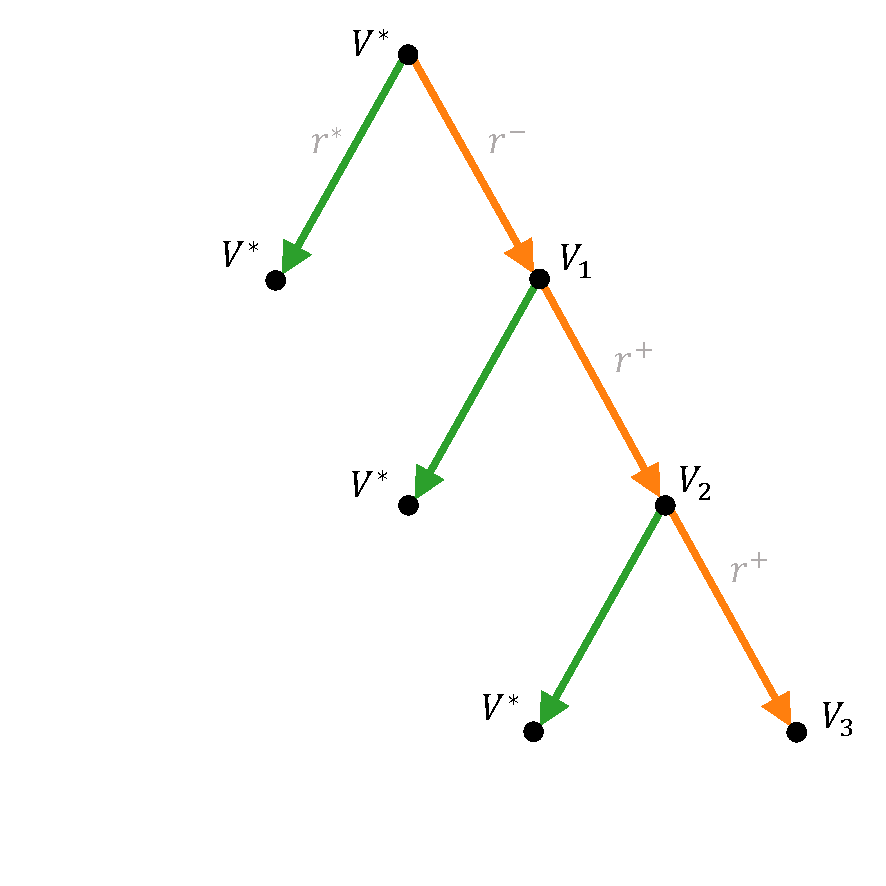
\includegraphics[trim={3.5cm 2cm 0.5cm 0.5cm}, clip, width=0.5\linewidth]{img/gbop/mdp_tree.pdf}
    \caption{Planning tree of the \gls{MDP} $\cM$ of \Cref{fig:mdp}}.
    \label{fig:mdp-tree}
\end{figure}
\begin{lemma}
	\begin{leftbar}[lemmabar]
 Any sequence of actions in $A\setminus{a_1}$ is in $\Tau^\infty$.
 \end{leftbar}
\end{lemma}
\begin{proof}
Any such sequence of actions yields the sequence of rewards $r^-, r^+, \dots,r^+$. and end up in the state $s^+$ with value at least $V^\star$ (obtained by further taking $a_1$ indefinitely). Thus its value $V_h$ verifies, 
\begin{align*}
    V_h &\geq \sum_{t=0}^{h-1} \gamma^t r_t + \gamma^h V^\star\\
    &= r^- - r^+ + \sum_{t=0}^{h-1} \gamma^t r^+ + \gamma^h V^\star \\
    &= (-\frac{\gamma}{1-\gamma} - 1)S + \frac{1-\gamma^h}{1-\gamma} (r^\star + S) + \gamma^h V^\star\\
    &= V^\star - S\frac{\gamma^h}{1-\gamma} \geq V^\star - \frac{\gamma^h}{1-\gamma}
\end{align*}
\end{proof}

We can directly conclude that $\kappa \geq \limsup{|\{a_2,\dots,a_K\}^h|^{1/h}} = K-1$.

Now, consider the nodes expanded by \GBOPD. The first expansion is that of the root, which discovers $s^\star$ and $s^+$. In the absence of information on these two state, the bound $V_{\max}$ is used and the first action $a_1$ gets a higher $\overline{U}$ that any other action $a_2,\dots,a_K$ since $r^\star \geq r^-$. Hence, at the second iteration, the node $a_1$ gets expanded. At this point, the self-loop of the state $s^\star$ is discovered, which means that form now on the bounds verify $L_n(a_1) = V^\star = U_n(a_1)$ for $n\geq2$, which means that $L_n(a_1\cA^*)-U_n(a_1\cA^*) = 0$. The nodes $a_2,\dots,a_K$ can be expanded at most once before the entire \gls{MDP} is discovered and $L_n=V=U_n$ over the entire tree, which means that $\Tau_n^\infty$ is the set of optimal nodes, \ie the nodes in the only optimal sequence $a_1^\star$. Hence, $\kappa_\infty = 1.$ 

\section{Time and memory complexities}

\subsection{\KLOLOP}
\label{sec:kl-olop-time}

After having considered the sample efficiency of \OLOP and \KLOLOP in \Cref{thm:regret-kl-olop}, we now study their time and memory complexities. We will only mention the case of \KLOLOP for ease of presentation, but all results easily extend to \OLOP.

The \Cref{alg:kl-olop} requires, at each episode, to compute and store in memory of the reward upper-bounds and U-values of all nodes in the tree $\Tau = \sum_{h=0}^L \cA^h$.
Hence, its time and memory complexities $C(\KLOLOP)$ are 
\begin{equation*}
C(\KLOLOP) = \cO(M|\Tau|) = \cO(MK^L).
\end{equation*}

The curse of dimensionality brought by the branching factor $K$ and horizon $L$ makes it intractable in practice to actually run \KLOLOP in its original form even for small problems. However, most of this computation and memory usage is wasted, as with reasonable sample budgets $n$ the vast majority of the tree $\Tau$ will not be actually explored and hence does not hold any valuable information.

We propose in \Cref{alg:lazy-kl-olop} a lazy version of \KLOLOP which only stores and processes the explored subtree, as shown in \Cref{fig:tree}, while preserving the inner workings of the original algorithm.

\begin{figure}[ht]
	\centering
	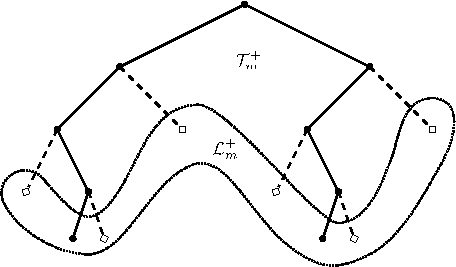
\includegraphics[width=0.6\textwidth]{img/tree_svg-tex}
	\caption{A representation of the tree $\Tau_m^+$, with $K = 2$ actions and after episode $m = 2$, when two sequences have been sampled. They are represented with solid lines and dots \textbullet, and they constitute the explored subtree $\Tau_m$. When extending $\Tau_m$ with the missing children of each node, represented with dashed lines and diamonds $\diamond$, we obtain the full extended subtree $\Tau_m^+$. The set of its leaves is denoted $\LL_m^+$ and shown as a dotted set.}
	\label{fig:tree}
\end{figure}

\begin{algorithm}[tp]
	\DontPrintSemicolon
	Let $M$ be the largest integer such that $M \log M/(2 \log 1/\discount) \leq n$\;
	Let $L = \log M / (2 \log 1/\discount)$\;
	Let $\Tau_0^+ = \LL_0^+ = \{\emptyset\}$\;
	\For{each episode $m = 1, \cdots, M$}{
		Compute $U_a(m-1)$ from \eqref{eq:Ua} for all $a\in\Tau_{m-1}^+$\;
		Compute $B_a(m-1)$ from \eqref{eq:Ba} for all $a\in \LL_{m-1}^+$\;
		Sample a sequence with highest B-value: $a \in \argmax_{a\in \LL_{m-1}^+} B_a(m-1)$\;
		Choose an arbitrary continuation $a^m \in \cA\cA^{L-|a|}$\tcp*{\eg uniformly}
		Let $\Tau_m^+ = \Tau_{m-1}^+$ and $\LL_m^+ = \LL_{m-1}^+$\;
		\For{$t=1, \cdots, L$}{
			\If{$a^m_{1:t} \not \in \Tau_{m}^+$}{
				Add $a^m_{1:t-1}A$ to $\Tau_{m}^+$ and $\LL_{m}^+$\;
				Remove $a^m_{1:t-1}$ from $\LL_{m}^+$
			}
		}
	}
	\Return the most played sequence $a(n) \in \argmax_{a\in \LL_m^+} N_a(m)$
	\caption{Lazy Open Loop Optimistic Planning}
	\label{alg:lazy-kl-olop}
\end{algorithm}


\begin{proposition}[Time and memory complexity]
	\begin{leftbar}[propositionbar]
		\Cref{alg:lazy-kl-olop} has time and memory complexities of
		\begin{equation*}
		C(\texttt{Lazy KL-OLOP}) = O(KLM^2)
		\end{equation*}
		
		The corresponding complexity gain compared to the original \Cref{alg:kl-olop} is: 
		\begin{equation*}
		\frac{C(\texttt{Lazy KL-OLOP})}{C(\KLOLOP)} = \frac{n}{K^{L-1}}
		\end{equation*}
		which highlights that only a subtree corresponding to the sample budget $n$ is processed instead of the search whole tree $\Tau$.
	\end{leftbar}
\end{proposition}
\begin{proof}
	At episode $m = 1, \cdots, M$, we compute and store in memory the reward upper-bounds and U-values of all nodes in the subtree $\Tau_m^+$. Moreover, the tree $\Tau_m^+$ is constructed iteratively by adding K nodes at most L times at each episode from 0 to $m$. Hence, $|\Tau_m^+| = O(mKL)$.
	This yields directly $C(\texttt{Lazy KL-OLOP}) = \sum_{m=1}^M O(mKL) = O(M^2KL)$.
\end{proof}

\begin{proposition}[Consistency]
	\label{prop:consistency}
	\begin{leftbar}[propositionbar]
		The set of sequences returned by \Cref{alg:lazy-kl-olop} is the same as the one returned by \Cref{alg:kl-olop}.
		In particular, \Cref{alg:lazy-kl-olop} enjoys the same regret bounds as in \Cref{thm:regret-kl-olop}.
	\end{leftbar}
\end{proposition}

\begin{proof}
	To prove consistency of \Cref{alg:lazy-kl-olop}, we need to show that the sequences of actions $a^m$ sampled at every episode are chosen arbitrarily from the same sets as in \Cref{alg:lazy-kl-olop}.
	Namely, 
	
	\begin{equation*}
	\left\{ b\in \cA \cA^{L-|a|} : a \in \argmax_{a\in \LL_{m-1}^+} B_a(m-1)\right\} = \argmax_{a\in \cA^L} B_a(m-1)
	\end{equation*}
	
	To that end, we first introduce some useful notations:
	
	\begin{paragraph}{Definition}
		\begin{leftbar}[defnbar]
			% We remind that $\Tau$ refers to the whole search tree $\Tau = \sum_{h=0}^L \cA^h$.
			Let $\Tau_m$ be the set of visited nodes after episode $m$:
			\begin{equation*}
			\Tau_m \eqdef \left\{a\in \cA^*: N_a(m) > 0\right\}
			\end{equation*}
			
			We also define its extension $\Tau_m^+$ of visited nodes and their children:
			\begin{equation*}
			\Tau_m^+ \eqdef \Tau_m + \Tau_m A
			\end{equation*}
			
			Now for $a\in \cA^*$, $\pi_m(a)$ (resp. $\pi_m^+(a)$) refers to its longest prefix within $\Tau_m$ (resp. $\Tau_m^+$):
			\begin{align*}
			\pi_m(a) &\eqdef \argmax_{b\in\Tau_m} \{|b|: a\in b \cA^* \} \\
			\pi_m^+(a) &\eqdef \argmax_{b\in\Tau_m^+} \{|b|: a\in b \cA^* \}
			\end{align*}
			
			Finally, $\LL_m$ and $\LL_m^+$ are the image of $\cA^L$ by $\pi_m$ and $\pi_m^+$, respectively.
			\begin{align*}
			\LL_m &\eqdef \pi_m(\cA^L) \\
			\LL_m^+ &\eqdef \pi_m^+(\cA^L) \}
			\end{align*}
		\end{leftbar}
	\end{paragraph}
	
	\begin{remark}[About children extensions]
		\begin{leftbar}[remarkbar]
			We could frame \Cref{alg:lazy-kl-olop} in terms of $\Tau_m$ and $\LL_m$, for which mathematical proofs are more straight-forward. However, the iterative construction of $\LL_m$ is tricky and it would require inverting $\pi_m$ on $\LL_m$ which is non-trivial. On the contrary, introducing their extensions  $\Tau_m^+$ and $\LL_m^+$ slightly complicates the proof, but greatly simplifies the construction of $\LL_m^+$ and the computation of ${\pi_m^+}^{-1}$ on $\LL_m^+$, which is why we use these sets in practice.
		\end{leftbar}
	\end{remark}
	
	\begin{lemma}[Sets construction]
		\begin{leftbar}[lemmabar]
			$\Tau_m^+$ and $\LL_m^+$ are indeed the sets computed in \Cref{alg:lazy-kl-olop}.
		\end{leftbar}
	\end{lemma}
	\begin{proof}
		Note that for each episode $1 \leq m \leq M - 1$, we have:
		\begin{equation}
		\label{eq:tau_mp1}
		\Tau_{m+1} = \Tau_{m} + \sum_{t=0}^L a^{m+1}_{1:t}
		\end{equation}
		Indeed, the nodes visited at least once at time $m+1$ where either already visited once at time $m$ (\eg in $\Tau_{m}$) or have been visited for the first time during episode $m+1$, which means they are a prefix of $a^{m+1}$. The reverse is clearly true as well.
		
		This enables to write:
		\begin{align*}
		\Tau_{m+1}^+ &= \Tau_{m+1} + \Tau_{m+1}A & \text{by definition}\\
		&= \Tau_{m} + \sum_{t=0}^L a^{m+1}_{1:t} + (\Tau_{m} + \sum_{t=0}^L a^{m+1}_{1:t})A & \text{by \eqref{eq:tau_mp1}} & \\
		&= (\Tau_{m} + \Tau_{m}A) + \sum_{t=0}^L a^{m+1}_{1:t} + \sum_{t=0}^L a^{m+1}_{1:t}A & \\
		&= \Tau_{m}^+ + a^{m+1}_{1:0} + \sum_{t=0}^L a^{m+1}_{1:t}A &\text{ as } \sum_{t=1}^L a^{m+1}_{1:t} \subset \sum_{t=0}^L a^{m+1}_{1:t}A\\
		&=  \Tau_{m}^+ + \sum_{t=0}^L a^{m+1}_{1:t}A  &\text{ as }a^{m+1}_{1:0}=\emptyset \in \Tau_{0} \subset \Tau_{m} \subset \Tau_m^+
		\end{align*}
		This recursion is the one implemented in \Cref{alg:lazy-kl-olop}: at each episode $m$, we add to $\Tau_{m}^+$ the children of the nodes along the sampled action sequence $a^{m}$.
		
		Finally, we highlight that $\LL_m^+ = \pi^+(\cA^L)$ is the set of leaves of $\Tau_{m}^+$.
		Indeed, nodes of $\LL_m^+$ belong to $\Tau_{m}^+$, but they cannot have a child in $\Tau_{m}^+$ as it would contradict the definition of $\LL_m^+$. Conversely, any leaf $a$ of $\Tau_{m}^+$ can be continued arbitrarily to a sequence $b$ of $\cA^L$, which  $a = \pi_m^+(b) \in \pi^+(\cA^L) = \LL_m^+$.
		
		Thus, when updating $\Tau_{m-1}^+$, the set of its leaves is updated accordingly: when the children of a leaf $a^m_{1:t-1}$ are added to $\Tau_m^+$, they become new leaves in place of their parent. Hence, they are added to $\LL_m^+$ while $a^m_{1:t-1}$ is removed from it.
		% 
	\end{proof}
	
	\begin{lemma}[U-values conservation]
		\begin{leftbar}[lemmabar]
			\label{lemma:value-conservation}
			For all $a \in \cA^*$,
			\begin{equation*}
			U_a(m) = U_{\pi_m(a)}(m) = U_{\pi_m^+(a)}(m)
			\end{equation*}
		\end{leftbar}
	\end{lemma}
	\begin{proof}
		Let $a \in \cA^*$, denote $h=|a|$ and $h'=|\pi_m(a)|$.
		
		By definition of $\pi_m(a)$, $0 \leq h' \leq h$, and
		\begin{itemize}
			\item for $1\leq t \leq h'$, we have $a_{1:t} = {\pi_m(a)}_{1:t}$ ;
			\item for $h'+1\leq t \leq h$, we have $a_{1:t} \not \in \Tau_m$, hence $T_{a_{1:t}}(m) = 0$ and $U^{\mu}_{a_{1:t}}(m) = 1$.
		\end{itemize}
		Then,
		\begin{align*}
		U_a(m) &= \sum_{t=1}^h \gamma^t U^{\mu}_{a_{1:t}}(m) + \frac{\gamma^{h+1}}{1-\gamma} \\
		&= \sum_{t=1}^{h'} \gamma^t U^{\mu}_{a_{1:t}}(m) + \sum_{t=h'+1}^h \gamma^t \underbrace{U^{\mu}_{a_{1:t}}(m)}_1 + \frac{\gamma^{h+1}}{1-\gamma} \\
		&= \sum_{t=1}^{h'} \gamma^t U^{\mu}_{{\pi_m(a)}_{1:t}}(m) + \frac{\gamma^{h'+1}}{1-\gamma} \\
		&= U_{\pi_m(a)}(m)
		\end{align*}
		
		Now, consider $\pi_m^+(a) \in \Tau_m^+$.
		By definition, it belongs either to $\Tau_m$ or $\Tau_m A$.
		\begin{itemize}
			\item If $\pi_m^+(a) \in \Tau_m$, then $\pi_m^+(a) = \pi_m(a)$ and $U_{\pi_m^+(a)}(m) = U_{\pi_m(a)}(m)$.
			\item Else, $\pi_m^+(a) \in \Tau_m A$ and $p(\pi_m^+(a)) = \pi_m(a)$.
			
			As $\pi_m^+(a) \not \in \Tau_m$, we have $T_{\pi_m^+(a)}(m) = 0$ and $U^{\mu}_{\pi_m^+(a)}(m) = 1$.
			This yields:
			
			\begin{equation*}
			U_{\pi_m^+(a)}(m) = \sum_{t=1}^{h'} \gamma^t U^{\mu}_{{\pi_m^+(a)}_{1:t}}(m) + \gamma^{h'+1} \underbrace{U^{\mu}_{{\pi_m^+(a)}}(m)}_1 + \frac{\gamma^{h'+2}}{1-\gamma} = U_{\pi_m(a)}(m)
			\end{equation*}
			
		\end{itemize}
		We showed that $U_{\pi_m^+(a)}(m) = U_{\pi_m(a)}(m)$, which concludes the proof.
		% 
	\end{proof}
	
	\begin{lemma}[Inverse projection]
		\begin{leftbar}[lemmabar]
			\label{lemma:inverse-proj}
			For all $a\in \LL_m^+$ of length $h\leq L$,
			\begin{equation*}
			{\pi_m^+}^{-1}(a) = a \cA^{L-h}
			\end{equation*}
			
			This allows to easily pick a sequence inside ${\pi_m^+}^{-1}(a)$: just continue the sequence $a$ with a default action of $A$ (\eg the first) until it reaches length $L$.
		\end{leftbar}
	\end{lemma}
	\begin{proof}
		Let $a\in \LL_m^+$. 
		
		By definition of $\pi_m^+$, any sequence in ${\pi_m^+}^{-1}(a)$ is a suffix of $a$ of length $L$, so we clearly have the direct inclusion ${\pi_m^+}^{-1}(a) \subset a \cA^{L-h}$.
		
		Now for the other side: let $b\in \cA \cA^{L-h}$, \ie $a=b_{1:h}$. We need to show that $\pi_m^+(b) = a$.
		As $a\in \LL_m^+$, there exists $c\in \cA^L$ such that $\pi_m^+(c) = a$.
		\begin{itemize}
			\item If h = L, then $b=a$, so $b \in \LL_m^+ \subset \Tau_m^+$, and hence $\pi_m^+(b)=b=a$.
			\item If h < L, we can show by contradiction that $a \not \in \Tau_m$. Indeed, if $a \in \Tau_m$, then $c_{1:h+1}$ is the child of a node of $\Tau_m$ and hence belongs to $\Tau_m^+$. But then, $c_{1:h+1}$ is a prefix of $c$ in $\Tau_m^+$ with greater length than $a$, which contradicts the definition of $a = \pi_m^+(c)$.
			
			Now, because $a \not \in \Tau_m$, it is also true for all suffixes of $a$, and in particular for $b_{1:t}$ with $h \leq t \leq L$. Indeed, we have $a^s_{1:t} = b_{1:t} \implies a^s_{1:h} = b_{1:h} = a$, so:
			\begin{equation*}
			T_{b_{1:t}}(m) = \sum_{s=1}^m \mathbbm{1}\{a^s_{1:t} = b_{1:t}\} \leq \sum_{s=1}^m \mathbbm{1}\{a^s_{1:h} = a\} = N_a(m) = 0
			\end{equation*}
			Hence, $b_{1:t} \not \in \Tau_m$ for all $h \leq t \leq L$, so in particular $b_{1:t} \not \in \Tau_m^+$ for all $h+1 \leq t \leq L$. Since $b_{1:h} = a \in \Tau_m^+$, $a$ is indeed the longest prefix of $b$ in $\Tau_m^+$, that is: $\pi_m^+(b) = a$.
		\end{itemize}
		We have shown the other side of the inclusion: $a \cA^{L-h} \subset {\pi_m^+}^{-1}(a)$, which entails that the two sets are in fact equal.
		% 
	\end{proof}
	
	We can now conclude our proof of \Cref{prop:consistency}: at episode $m$, \KLOLOP samples a sequence of action $a^m$ within the set $\argmax_{a\in \cA^L} U_a(m)$. 
	However, we have:
	
	\begin{align*}
	\argmax_{c\in \cA^L} U_c(m) &= \argmax_{c\in \cA^L} U_{\pi_m^+(c)}(m) & \text{by \Cref{lemma:value-conservation}} \\
	&= {\pi_m^+}^{-1}\left(\argmax_{a\in {\pi_m^+}(\cA^L)} U_{a}(m)\right) & \\
	&= \left\{b\in{\pi_m^+}^{-1}(a) : a\in \argmax_{a\in \LL_m^+} U_{a}(m)\right\} & \\
	&= \left\{b\in \cA \cA^{L-|a|} : a\in \argmax_{a\in \LL_m^+} U_{a}(m)\right\} & \text{by \Cref{lemma:inverse-proj}} 
	\end{align*}
	
	Thus, at each episode the sequence of actions $a^m$ sampled by \Cref{alg:lazy-kl-olop} could have been sampled by \Cref{alg:kl-olop} as well.
	
	In particular, if the arbitrary rule used to pick a sequence from a set is the same for the two algorithms, then the sampled sequences $a^m$ will be identical, will have the same visit count $T_{a^m}(m)$, and in the end the returned action $a(n)$ will be the same.
	% 
\end{proof}

\subsection{\GBOP}
\label{sec:gbop-implementation}

In this section, we provide more details about the implementation of \GBOPD and \GBOP. First, we discuss how two procedures can be approximated so that they terminate in finite time, and study the impact of this approximation on the regret guarantees. Second, we propose a lazy implementation of the bounds computation through $\cB_n^\infty$ that only considers a subset of nodes to update.

\subsubsection{Termination}

\paragraph{Bounds computation}

The bounds computation step $\cB_n^\infty$ (line 1 of \GBOPD) can converge in infinite time whenever $\cG_n$ contains a loop, as shown in \Cref{fig:simple_loop}. We consider the effect of stopping early after a fixed number of iterations $k(\varepsilon,\gamma)$.

\begin{figure}[th]
	\centering
	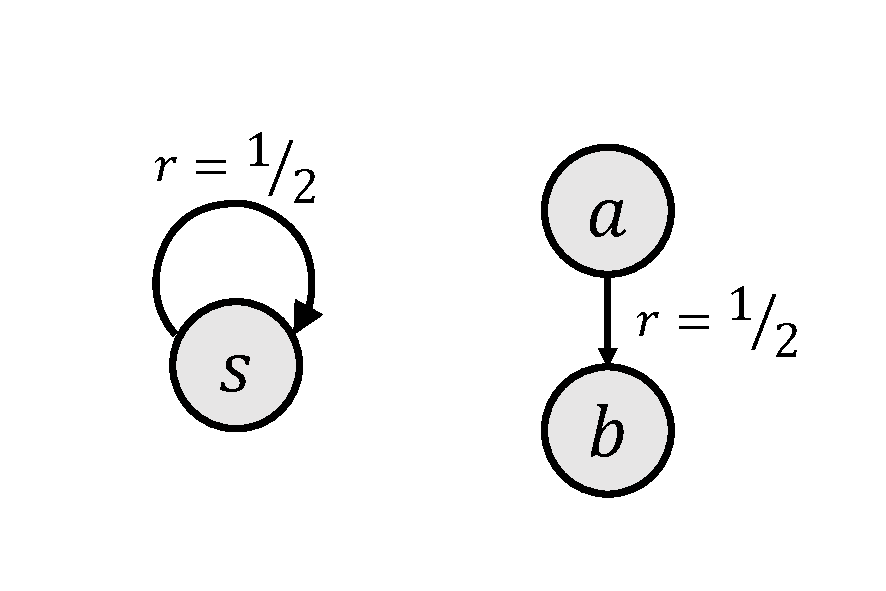
\includegraphics[trim=2.5cm 1cm 9cm 2cm, clip, width=0.1\linewidth]{img/gbop/loop.pdf}\\
	\begin{tabular}{lccccc}
		\toprule
		$k$ & $0$ & $1$ & $\cdots$ & $k$ \\
		\midrule
		$\cU = \cB^k(V_{\max})(s)$ & $V_{\max}$ & $\frac{1}{2} + \gamma V_{\max}$ && $\frac{1}{2}(1-\gamma^k)V_{\max} + \gamma^k V_{\max}$\\
		$\cL = \cB^k(0)(s)$ & $0$ & $\frac{1}{2}$ && $\frac{1}{2}(1-\gamma^k)V_{\max}$\\
		\bottomrule
	\end{tabular}
	\caption{\textbf{Top}: a simple looping MDP with $|S|=|A|=1$ after having observed a single transition ($n=1$). \textbf{Bottom}: the sequence of bounds $\cB_1^k(0)$ and $\cB_1^k(V_{\max})$. They converge geometrically to their limit $\cU_1 = \cL_1 = V = \frac{1}{2}V_{\max}$, thus in infinite time.}
	\label{fig:simple_loop}
\end{figure}

\begin{proposition}[Time complexity of bounds computation]
	\begin{leftbar}[propositionbar]
		An $\varepsilon$-approximation of $(\cL_n, \cU_n)$ can be computed by applying $\cB_n$ for a finite number $k(\epsilon,\gamma)$ of iterations, with $$k(\epsilon,\gamma) = \log_\gamma\frac{1}{\varepsilon(1-\gamma)}.$$ 
	\end{leftbar}
\end{proposition}
\begin{proof}
	$\cB_n$ is a $\gamma$-contraction by \Cref{lem:properties-b-graph}, and $\cU_n$ (resp $\cL_n$) is at a distance (in $\|\dot\|_\infty$) at most $V_{\max}$ of the initial value bound $V_{\max}$ (resp $0$). Thus, the $k^{\text{th}}$ application of $\cB_n$ decreases this error by a factor $\gamma^k$, which gives the result.
\end{proof}

The impact of using an $\varepsilon$-approximation of $(\cL_n, \cU_n)$ during planning is the following:
\begin{proposition}[Effect of early stopping]
	\begin{leftbar}[propositionbar]
		\label{prop:early-stopping}
		Denote the approximate bounds $(\hat{\cL}_n, \hat{\cU}_n)$ obtained by applying $\cB_n^{k(\varepsilon,\gamma)}$ instead of $\cB_n^\infty$, and likewise $(\hat{L}_n, \hat{U}_n)$ in their tree version obtained by applying $B_n^{k(\varepsilon,\gamma)}$ instead of $B_n^\infty$.
		Then, running \GBOPD with $\hat{\cL}_n, \hat{\cU}_n$ gives the following regret:
		\begin{align*}
		\regret = \tilde{\cO}\left(n^{-\log \frac{1}{\gamma}/\hlob{\log \hat{\kappa}_\infty}}\right),
		\end{align*}
		with $$\hlgb{{\kappa}_\infty} \leq \hlob{\hat{\kappa}_\infty \eqdef \lim_{n\rightarrow\infty} \kappa(\hat{L}_n, \hat{U}_n)} \leq \hlrb{\kappa}.$$
		Moreover, the approximation gap $\hlgb{\kappa_\infty} - \hlob{\hat{\kappa}_\infty}$ is non-increasing with respect to $\varepsilon$.
	\end{leftbar}
\end{proposition}
It is difficult to control more explicitly the gap between $\hlgb{\kappa_\infty}$ and $\hlob{\hat{\kappa}_\infty}$, which might be discontinuous with $\varepsilon$.

\begin{proof}
	Note that $\hat{L}_n$ and $\hat{U}_n$ are valid monotonic bounds on $V$, verifying
	\[0\leq \hat{L}_n\leq {L}_n \leq V \leq {U}_n\leq \hat{U}_n \leq V_{\max}.\]
	Thus, \Cref{lem:bounds} holds with the difference that we only have an inequality $$\overline{U_n}(a) \geq \max_{a'\in a \cA^\infty} \overline{U}(a')$$ rather than an equality, by monotonicity but non-invariance by $B_n$. However, this was the actual inequality used in \Cref{lem:expansion-bound}, which still holds by replacing $L_n,U_n$ by their approximation $\hat{L}_n,\hat{U}_n$. Likewise, \Cref{lem:recommendation-bound} holds. The proof of \Cref{thm:regret-gbop}, can be written with the modification that expanded nodes belong to $T_h^\infty(\hat{L}_n, \hat{U}_n))$, which gives the claimed bound.
	
	As $\varepsilon$ decreases, $k(\epsilon,\gamma)$ increases, which means by \Cref{lem:properties-b-tree} that $(\hat{\cL}_n, \hat{\cU}_n)$ get tighter and $\hlob{\hat{\kappa}_\infty}$ shrinks by \Cref{lem:shrink}. It reaches its minimum $\hlgb{\kappa_\infty}$ when $\varepsilon=0$.
\end{proof}

Thus, we observe that there is a \emph{tradeoff} between the time complexity $k(\varepsilon)$ and the sample complexity $\hlob{\hat{\kappa}_\infty}$: decreasing one increases the other.

Note that \OPD uses $d_n$ iterations of $B_n$, which corresponds to a tuning of $\varepsilon$ with $n$: $\varepsilon_n = \frac{\gamma^{d_n}}{1-\gamma} = \cO(n^{-\frac{\log 1/\gamma}{\log \kappa}})$. 


\paragraph{Sampling rule}

The sampling rule of \GBOPD (line 2 of \GBOPD) can yield an infinite sequence $b_n$. We propose to stop the sampling after a fixed depth $d^+_n$.

\begin{proposition}[Time complexity of sampling]
	\begin{leftbar}[propositionbar]
		Consider the variant of \GBOPD where we stop the sampling rule when reaching a fixed depth $d^+_n$ chosen polynomial with $n$:
		\[d^+_n = \ceil{\alpha n^\beta},\; \text{with }\alpha,\beta > 0\]
		Then, the regret bound of \Cref{thm:regret-gbop} (or that of \Cref{prop:early-stopping} when using early stopping in the bounds computation) still holds.
	\end{leftbar}
\end{proposition}

Note that this is not too constraining compared to \OPD, for which the sampling rule complexity $d_n$ is upper-bounded by $n$. Hence, by choosing $\alpha=\beta=1$, \GBOPD preserve the same complexity as \OPD in the worst case.

\begin{proof}
	Let $\kappa'>\hlgb{{\kappa}_\infty}$ (or $\kappa'>\hlob{\hat{\kappa}_\infty}$ under approximate bounds). In the proof of \Cref{thm:regret-gbop}, it is shown that the maximum depth $d_n$ of an expanded node is at least $d^-_n \eqdef \log_{\kappa'}\frac{n-C_0}{C_1'}$, which allows to conclude with \Cref{lem:recommendation-bound} that $\regret = \cO(\gamma^{d_n}) = \cO(\gamma^{d^-_n})$. By choosing $d^+_n$ polynomial, we have that $d^+_n$ is greater than $d^-_n$ for $n$ sufficiently high. Thus, by stopping the sampling after reaching a depth $d^+_n$, we have that $\regret \leq \gamma^{\min\{d_n, d^+_n\}} / (1-\gamma) = \cO(\gamma^{d^-_n}) = \cO(n^{\frac{-\log 1/\gamma}{\log \kappa'}})$
\end{proof}

\subsubsection{Efficient implementation of $\cB_n^\infty$}

The bounds $\cL_n$ and $\cU_n$ are computed by fixed-point iteration of $\cB_n$ from the trivial bounds $(0,V_{\max})$. The naive implementation of $\cB_n$ requires to iterate over the whole set of state-action pairs in $\cG_n$. 
Two ideas can be used to increase the efficiency of both steps:
\begin{enumerate}[label=(\roman*)]
	\item Instead of starting the iteration with the trivial bounds, the previous estimate $\cL_{n-1}, \cU_{n-1}$ can be used instead at iteration $n$. Since these bounds are closer to their limit ($0\leq \cL_{n-1}\leq \cL_n$ and $\cU_n\leq \cU_{n-1} \leq V_{\max}$), the fixed-point iteration will converge quicker.
	\item In particular, since $\cL_{n-1}$ and $\cU_{n-1}$ are invariant by $\cB_n$, the the only nodes modified by a supplementary application of $\cB_n$ are the parents of only updated node: the expanded state $s_n$. Once its value is updated by $\cB_n$, the same reasoning can be applied for the next iteration of $\cB_n$: only its predecessors can be updated. Thus, we can keep track of a set $q$ of states that can be updated, for every application of $\cB_n$.
\end{enumerate}
These idea are formalised in \Cref{alg:queue-b-inf}. Note that the criterion $\|\cB_n^{k+1} - \cB_n^k\| \leq \frac{1-\gamma}{\gamma}\varepsilon$ is used to detect that the limit $\cB_n^\infty$ is approximated with accuracy $\varepsilon$, and stems from $\cB_n$ being a $\gamma$-contraction:
\begin{proof}
	$\|\cB_n^k - \cB_n^\infty\| \leq \gamma\| \cB_n^{k+1} - \cB_n^\infty\| \leq \gamma \|\cB_n^{k+1} - \cB_n^{k}\| + \gamma \|\cB_n^{k} - \cB_n^\infty\|$, with $\| \cB_n^{k+1} - \cB_n^{k}\| \leq \frac{1-\gamma}{\gamma}\varepsilon$, thus $\|\cB_n^{k} - \cB_n^\infty\| \leq \varepsilon$.
\end{proof}

\begin{algorithm}
	\caption{A queue-based implementation of $\cB_n^\infty$.}
	\label{alg:queue-b-inf}
	\KwIn{Initial bound $\cU_{n-1}$, expanded node $s_n$, accuracy $\varepsilon$}
	\KwOut{An $\varepsilon$-approximation of $\cU_{n}$}
	\DontPrintSemicolon
	$\cU_n \gets \cU_{n-1}$\;
	$q\gets [s_n]$\;
	\While{$q$ is not empty}{
		$s'\gets$ Pop the first node from the queue $q$\;
		$\cU' \gets \cB_n(\cU_n)(s')$\Comment*[r]{Node backup}
		\If(\Comment*[f]{Stopping rule}){$\cU' - \cU_n > \frac{1-\gamma}{\gamma}\varepsilon$}{
			Push the predecessors $s$ of $s'$ to the queue $q$ \Comment*[r]{Propagation rule}
		}
		$\cU_n(s') \gets \cU'$\;
	}
	\Return $\cU_n$\;
\end{algorithm}


	%!TEX root = ../../PhD_thesis__Edouard_Leurent.tex
\graphicspath{{2-Chapters/7-Chapter/}}
	
\chapter{Complements on \Cref{chapter:7}}
	\section{Proofs}
	
	\subsection{Proof of \Cref{prop:regularized_solution}}
	\label{sec:proof-regularized_solution}
	
	\begin{proof}
		We differentiate $J(\theta) = \sum_{n=1}^N \|y_n -\Phi_n\theta\|_{\Sigma_p^{-1}}^2 + \lambda\|\theta\|_{}^2$ as in  \eqref{eq:regression_min} with respect to $\theta$:
		
		\begin{align*}
		\nabla_{\theta} J(\theta) &= \sum_{n=1}^N\nabla_{\theta} (y_n - \Phi_n\theta)^\transp\Sigma_p^{-1}(y_n - \Phi_n\theta) + \nabla_{\theta} \lambda\|\theta\|_{}^2\\
		&= -2\sum_{n=1}^N y_n^\transp\Sigma_p^{-1}\Phi_n + 2\sum_{n=1}^N\theta^\transp(\Phi_n^\transp\Sigma^{-1}\Phi_n) +  2 \lambda \theta^\transp
		\end{align*}
		
		Hence,
		\begin{align*}
		\nabla_{\theta} J(\theta) = 0 \iff \left(\sum_{n=1}^N\Phi_n^\transp\Sigma_p^{-1}\Phi_n + I_d\right)\theta = \sum_{n=1}^N y_n^\transp\Sigma_p^{-1}\Phi_n
		\end{align*}
	\end{proof}
	
	\subsection{Proof of \Cref{thm:confidence_ellipsoid}}
	\label{sec:proof-confidence_ellipsoid}
	
	We start by showing a preliminary proposition:
	\newpage
	
	\begin{proposition}[Matrix version of Theorem 1 of \citealp{Abbasi2011}]
		\label{prop:concentration}
		\begin{leftbar}[propositionbar]
		Let $\{F_n\}_{n=0}$ be a filtration.
		Let $\{\eta_n\}_{n=1}^\infty$ be a $\Real^p$-valued stochastic process such that $\eta_n$ is $F_n$-measurable and $\expectedvalue\left[\eta_n\condbar F_{n-1}\right]$ is $\Sigma_p$-sub-Gaussian.
		
		Let $\{\Phi_n\}_{n=1}^\infty$ be an $\Real^{p\times d}$-valued stochastic process such that $\Phi_n$ is $F_n$-measurable. Assume that $G$ is a $d\times d$ positive definite matrix.
		For any $n\geq 0$, define
		\begin{equation*}
		\overline{G}_n = G + \sum_{s=1}^n \Phi_s^\transp \Sigma_p^{-1} \Phi_s \in \Real^{d\times d} \quad S_n = \sum_{s=1}^n \Phi_s^\transp\Sigma_p^{-1}\eta_s \in \Real^{d}.
		\end{equation*}
		Then, for any $\confidence>0$, with probability at least $1-\confidence$, for all $n\geq0$,
		\begin{align*}
		\| S_n \|_{\overline{G}_n^{-1}} \leq \sqrt{2\log \left(\frac{\det\left(\overline{G}_n\right)^{1/2}}{\confidence\det(G)^{1/2}}\right)}.
		\end{align*}
		\end{leftbar}
	\end{proposition}
	\begin{proof}
		Let 
		\begin{equation*}
		G_t = \sum_{s=1}^t \Phi_s^\transp \Sigma_p^{-1} \Phi_s \in \Real^{d\times d}
		\end{equation*}
		And for any $z\in\Real^d$,
		\begin{equation*}
		M_t^z = \exp{\left(\inp{z}{S_t} - \frac{1}{2}\|z\|_{G_t}\right)}
		\end{equation*}
		\begin{equation*}
		D_t^z = \exp{\left(\inp{\Phi_t z}{\eta_t}_{\Sigma_p^{-1}} - \frac{1}{2}\|\Phi_t z\|_{\Sigma_p^{-1}}\right)}
		\end{equation*}
		Then,
		\begin{align*}
		M_t^z &= \exp{\left(\sum_{s=1}^t z^\transp \Phi_s^\transp \Sigma_p^{-1} \eta_s - \frac{1}{2} (\Phi_s z)^\transp\Sigma_p^{-1}(\Phi_s z) \right)} \\
		&= \prod_{s=1}^{t} D_s^z
		\end{align*}
		and using the sub-Gaussianity of $\eta_t$
		\begin{align*}
		\expectedvalue\left[D_t^z \condbar F_{t-1}\right] = {}& \exp{\left(- \frac{1}{2}\|\Phi_t z\|_{\Sigma_p^{-1}}\right)}\\ &\expectedvalue\left[\exp{\left(\inp{\Phi_t z}{\eta_t}_{\Sigma_p^{-1}}\right)} \condbar F_{t-1}\right]  \\
		\leq {} & \exp{\left(- \frac{1}{2}\|\Phi_t z\|_{\Sigma_p^{-1}}\right)}\\
		&\exp{\left((z^\transp \Phi_t^\transp \Sigma_p^{-1})\Sigma_p(\Sigma_p^{-1} \Phi_t z)\right)}\\
		&= 1
		\end{align*}
		\begin{align*}
		\expectedvalue\left[M_t^z \condbar F_{t-1}\right] = \left(\prod_{s=1}^{t-1} D_s^z\right) \expectedvalue\left[D_t^z \condbar F_{t-1}\right] \leq M_{t-1}^z
		\end{align*}
		Showing that $(M_t^z)_{t=1}^\infty$ is indeed a supermartingale and in fact $\expectedvalue[M_t^z]\leq 1$.
		It then follows by Doob's upcrossing lemma for supermartingale that $M_\infty^z = \lim_{t\to\infty} M_t^z$ is almost surely well-defined, and so is $M_\tau^z$ for any random stopping time $\tau$.
		
		Next, we consider the stopped martingale $M_{\min(\tau,t)}^z$. Since 
		$(M_t^z)_{t=1}^\infty$ is a non-negative supermartingale and $\tau$ is a random stopping time, we deduce by Doob's decomposition that
		\begin{align*}
		\expectedvalue[M_{\min(\tau,t)}^z] &= \expectedvalue[M_0^z] + \expectedvalue[\sum_{s=0}^{t-1} (M_{s+1}^z-M_s^z) \mathbb{I}\{\tau>s\}]\\
		&\leq 1 + \expectedvalue[\sum_{s=0}^{t-1} \expectedvalue[M_{s+1}^z-M_s^z|F_{s}] \mathbb{I}\{\tau>s\}]\\
		&\leq 1
		\end{align*}
		Finally, an application of Fatou's lemma show that 
		$$\expectedvalue[M_\tau^z] = \expectedvalue[\liminf_{t\to\infty} M_{\min(\tau,t)}^z] \leq \liminf_{t\to\infty} \expectedvalue[M_{\min(\tau,t)}^z] \leq 1.$$
		
		This results allows to apply a result from \citep{pena2008self}.
		\begin{lemma}[Theorem 14.7 of \citealp{pena2008self}]
			\begin{leftbar}[lemmabar]
			If $Z$ is a random vector and $B$ is a symmetric positive definite matrix such that
			\[\forall \discount\in\Real^d, \log \expectedvalue \exp \left(\discount^\transp Z -\frac{1}{2} \discount^\transp B \discount \right)\leq 0,\]
			then for any positive definite non-random matrix C, it holds
			\[\expectedvalue\left[ \sqrt{\frac{\det(C)}{\det(B+C)} } \exp\left( \frac{1}{2}\|Z\|^2_{(B+C)^{-1}}\right)\right]\leq 1. \] 
			In particular, by Markov inequality, for all $\confidence\in(0,1)$, 
			\[\probability{\|Z\|_{(B+C)^{-1}} \geq \sqrt{2\log \left(\frac{\det \left((B+C)^{1/2}\right)}{\confidence\det(C)^{1/2}}\right)}}\leq \confidence.\]
			\end{leftbar}
		\end{lemma}
		
		Here, by using $Z = \sum_{s=1}^t\Phi_s\Sigma_p^{-1}\eta_s$, $B=G_t$, $C=G$,
		
		\[
		\probability{\| S_t \|_{(G_t+G)^{-1}} \geq \sqrt{2\log \left(\frac{\det(G_t+G)^{1/2}}{\confidence\det(G)^{1/2}}\right)}} \leq \confidence
		\]
		
	\end{proof}
	
	Having shown this preliminary result, we move on to the proof of \Cref{thm:confidence_ellipsoid}.
	
	\begin{proof}
		For all $x\in\Real^d$, \eqref{eq:vector_rls} gives
		\begin{align*}
		x^\transp\theta_{N,\lambda}  -x^\transp\theta &= x^\transp G_{N, \lambda}^{-1}\sum_{n=1}^N \Phi_n^\transp \Sigma_p^{-1}\eta_n
		- \lambda x^\transp G_{N, \lambda}^{-1}\theta\\
		&= \inp{x}{\sum_{n=1}^N \Phi_n^\transp \Sigma_p^{-1}\eta_n}_{G_{N, \lambda}^{-1}} - \lambda\inp{x}{\theta}_{G_{N, \lambda}^{-1}}
		\end{align*}
		
		Using the Cauchy-Schwartz inequality, we get
		\begin{align*}
		|x^\transp\theta_{N,\lambda}  -x^\transp\theta| \leq \|x\|_{G_{N, \lambda}^{-1}}\left(\left\|\sum_{n=1}^N \Phi_n^\transp \Sigma_p^{-1}\eta_n\right\|_{G_{N, \lambda}^{-1}} + \lambda\|\theta\|_{G_{N, \lambda}^{-1}}\right)
		\end{align*}
		
		In particular, for $x = G_{N,\lambda}(\theta_{N,\lambda} - \theta)$, we get after simplifying with $\| \theta_{N,\lambda}  - \theta\|_{G_{N,\lambda}}$,
		\begin{align*}
		\| \theta_{N,\lambda}  - \theta\|_{G_{N,\lambda}} &\leq \left\|\sum_{n=1}^N \Phi_n^\transp \Sigma_p^{-1}\eta_n\right\|_{G_{N, \lambda}^{-1}} + \lambda\|\theta\|_{G_{N, \lambda}^{-1}}
		\end{align*}
		
		By applying \Cref{prop:concentration} with $G=\lambda I_d$, we obtain that with probability at least $1-\confidence$,
		\begin{align*}
		\| \theta_{N,\lambda}  - \theta\|_{G_{N,\lambda}} &\leq \sqrt{2\log \left(\frac{\det(G_{N,\lambda})^{1/2}}{\confidence\det(\lambda I_d)^{1/2}}\right)}
		+ \lambda\|\theta\|_{G_{N, \lambda}^{-1}}
		\end{align*}
		And since $\|\theta\|_{G_{N, \lambda}^{-1}}^2 \leq 1/\lambda_{\min}(G_{N,\lambda})\|\theta\|_2^2 \leq 1/\lambda \|\theta\|_2^2$ and $\|\theta\|_2^2 \leq d\|\theta\|_\infty^2\leq d S^2$,
		\begin{align*}
		\| \theta_{N,\lambda}  - \theta\|_{G_{N,\lambda}} &\leq \sqrt{2\log \left(\frac{\det(G_{N,\lambda})^{1/2}}{\confidence\det(\lambda I_d)^{1/2}}\right)}
		+ (\lambda d)^{1/2}S
		\end{align*}
	\end{proof}
	
	
	\subsection{Proof of \Cref{prop:lower-bound}}
	\label{sec:proof-lower-bound}
	\begin{proof}
		The predictor designed in \Cref{sec:prediction} verifies the inclusion property \eqref{eq:inclusion-property}. Thus, for sequence of controls $\bu$, any dynamics $\structureddynamics\in C_{[N],\confidence}$, and perturbations $\underline{\bom} \leq \bom \leq \overline{\bom}$, the corresponding state at time $t_n$ is bounded by $\underline{x}_n \leq x_n \leq \overline{x}_n$, which implies that $R(x_n) \geq \min_{x\in[\underline{x}_n(\bu), \overline{x}_n(\bu)]}  R(x) = \pessimisticreward_n(\bu)$.
		
		Thus, by taking the min over $C_{[N],\confidence}$ and $[\underline{\bom}, \overline{\bom}]$, we also have for any sequence of controls $\bu$,
		\begin{align*}
		V^r(\bu) &= \min_{\substack{\structureddynamics\in C_{[N],\confidence}\\ \underline{\bom} \leq \bom \leq \overline{\bom}}} \sum_{n=N+1}^\infty \discount^n R(x_n)\\
		&\geq \sum_{n=N+1}^\infty \discount^n \pessimisticreward_n(\bu)\\
		&= \hat{V}^r(\bu)
		\end{align*}
	\end{proof}
	
	\subsection{Proof of \Cref{thm:minimax-regret-bound}}
	\label{sec:proof-minimax-regret-bound}
	We first bound the model estimation error.
	\begin{lemma}
	\label{lem:dynamics-est-bound}
	\begin{leftbar}[lemmabar]
		\[\|\structureddynamics - A(\theta_{[N],\lambda})\|_2 = \cO\left(\sqrt{ {\frac{\beta_N(\delta)^2}{\lambda_{\min}(\gramian)}}}\right) \]
	\end{leftbar}
	\end{lemma}
	\begin{proof}
		We have 
		\begin{align*}
		\|\theta - \theta_{[N],\lambda}\|_{G_{[N],\lambda}}^2 \geq \lambda_{\min}(\gramian)\|\theta - \theta_{[N],\lambda}\|_{2}^2
		\end{align*}
		And \eqref{eq:confidence-ellipsoid} gives
		\[\|\theta - \theta_{[N],\lambda}\|_{G_{[N],\lambda}}^2 = \cO(\beta_N(\delta)^2) \]
		
		Moreover, $\structureddynamics$ belongs to a linear image of this $L^2$-ball. By writing a the $j^{th}$ column of a matrix $M$ as $M_j$, and its coefficient $i,j$ as $M_{i,j}$,
		\begin{align*}
		((\structureddynamics&-A(\theta_{[N],\lambda}))^\transp (\structureddynamics - A(\theta_{[N],\lambda})))_{i,j}\\
		%&= (\phi_i(\theta-\theta_{[N],\lambda}))^\transp \phi_j(\theta-\theta_{[N],\lambda}) \\
		&= (\theta-\theta_{[N],\lambda})^\transp\phi_{i}^{\transp}\phi_j(\theta-\theta_{[N],\lambda}) \\
		&\leq \lambda_{\max}(\phi_{i}^{\transp}\phi_j) \|\theta - \theta_{[N],\lambda}\|_{2}^2 = \cO\left( {\frac{\beta_N(\delta)^2}{\lambda_{\min}(\gramian)}}\right) 
		\end{align*}
		
	\end{proof}
	
	Then, we propagate this estimation error through the state prediction.
	
	\begin{lemma}
		\begin{leftbar}[lemmabar]
		If there exist $P>0,Q_0\in\Real^{p\times p}$, $\rho>0$ such that
		\begin{align*}
		\begin{bmatrix}
		A_0^\transp P + P A_0^\transp + Q_0 & P|D|  \\
		|D|^\transp P & -\rho I_r \\
		\end{bmatrix}< 0,
		\end{align*}
		then for all $t> t_N$,
		\[\|\ox(t) - \ux(t)\| \leq \left(C_0 + \cO\left({\frac{\beta_N(\delta)^2}{\lambda_{\min}(\gramian)}} \right)\right)C_\omega(t), \]
		where $$C_0 = \sqrt{\frac{2\rho\lambda_{\max}(P)}{\lambda_{\min}(P)\lambda_{\min}(Q_0)}},$$ and $$C_\omega(t) = \sup_{\tau\in[t_N,t]} \|\overline{\omega}(\tau) - \underline{\omega}(\tau)\|_2^2.$$
		\end{leftbar}
	\end{lemma}
	\begin{proof}
		Let $e = \ox - \ux$. \eqref{eq:interval-predictor} gives the dynamics
		\begin{align*}
		\dot{e} = A_0e + |\Delta A|(\ox^+ + \ux^-) + |D|(\overline{\omega} - \underline{\omega})
		\end{align*}
		where recall that $|M| = M^+ + M^-$ for any matrix $M\in\Real^{p\times p}$.
		
		We define the Lyapunov function $V = e^\transp P e$, which is non-negative definite provided that
		$
		P>0,
		$ and compute its derivative
		\begin{align*}
		\dot{V} ={}& X^\transp
		\begin{bmatrix}
		A_0^\transp P + P A_0^\transp + Q & P|D| & P|\Delta A| \\
		|D|^\transp P & -\rho I_r & 0\\
		|\Delta A|^\transp P & 0 & -\alpha I_p
		\end{bmatrix}
		X\\
		& - e^\transp Q e + \alpha |\ux^+ + \ox^-|^2 + \rho |\overline{\omega} - \underline{\omega}|^2
		\end{align*}
		with $X=\begin{bmatrix}
		e & \overline{\omega} - \underline{\omega} &  \ux^+ + \ox^-
		\end{bmatrix}^\transp$, for any $Q\in\Real^{p\times p}$, $\rho,\alpha\in\Real$ . 
		
		Moreover, it holds that $-\ux^+ -\ox^- \leq e \leq \ox^+ + \ux^-$, which implies $|\ux^+ + \ox^-| \leq 2 |e|$. Hence,
		\begin{align*}
		\dot{V} \leq {}& X^\transp
		\underbrace{
			\left[
			\begin{array}{cc|c}
			A_0^\transp P + P A_0^\transp + Q + 4\alpha I_p & P|D| & P|\Delta A| \\
			|D|^\transp P & -\rho I_r & 0\\
			\hline
			|\Delta A|^\transp P & 0 & -\alpha I_p
			\end{array}
			\right]}_{\Upsilon}
		X\\
		& - e^\transp Q e + \rho \|\overline{\omega} - \underline{\omega}\|_2^2
		\end{align*}
		
		Thus, if we had $\Upsilon \leq 0$, $Q>0$, $\rho > 0$, then we would have
		\[
		\dot{V} \leq -\mu V + \rho \|\overline{\omega} - \underline{\omega}\|_2^2
		\]
		with $\mu = \frac{\lambda_{\min}(Q)}{\lambda_{\max}(P)}$. Since $V(t_N) = 0$, this further implies that for all $t>t_N$, 
		\begin{equation}
		\label{eq:lyap-bound}
		V(t) \leq \frac{\rho}{\mu} C_\omega(t)
		\end{equation}
		
		We now examine the condition $\Upsilon \leq 0$.
		We resort to its Schur complement: given $\alpha > 0$, $\Upsilon \leq 0$ if and only if $R \geq S$, where $S= \alpha^{-1}\begin{bmatrix}|\Delta A|^\transp P & 0\end{bmatrix}^\transp \begin{bmatrix}|\Delta A|^\transp P & 0\end{bmatrix}$ and $R$ is the top-left block of $-\Upsilon$:
		\[R = \begin{bmatrix}
		-A_0^\transp P - P A_0^\transp - Q - 4\alpha I_p & -P|D|\\
		-|D|^\transp P & \rho I_r\\
		\end{bmatrix}\]
		
		Choose $Q = \frac{1}{2}Q_0-4\alpha I_p$.
		Assume that $P$ is fixed and satisfies the conditions of the lemma. We have $$\lambda_{\max}(S) \leq \alpha^{-1}\lambda_{\max}(|\Delta A|)^2\lambda_{\max}(P)^2.$$
		
		Thus, by taking $\alpha = \frac{\lambda_{\max}(|\Delta A|)^2\lambda_{\max}(P)^2}{2\lambda_{\min}(Q_0)} = \cO({\frac{\beta_N(\delta)^2}{\lambda_{\min}(\gramian)}})$, we can obtain that $S \leq \begin{bmatrix}
		\frac{1}{2}Q_0 & 0\\0 & 0
		\end{bmatrix}$. Thus,
		\[R-S \geq \begin{bmatrix}
		-A_0^\transp P - P A_0^\transp - Q_0 & -P|D|\\
		-|D|^\transp P & \rho I_r\\
		\end{bmatrix} > 0 \]
		as it is assumed in the conditions of the lemma. Hence, under such a choice of $\alpha$ and $Q$, we recover $\Upsilon\leq 0$. \eqref{eq:lyap-bound} follows with $\mu = \frac{\lambda_{\min}(Q)}{\lambda_{\max}(P)} = \frac{\frac{1}{2}\lambda_{\min}(Q_0) - 4\alpha}{\lambda_{\max}(P)}$.
		Finally, we obtain
		\begin{align*}
		\|e(t)\|_2^2 &\leq \lambda_{\min}(P)^{-1} V(t)\\
		& \leq \frac{2\rho\lambda_{\max}(P)/\lambda_{\min}(P)}{\lambda_{\min}(Q_0) - 8\alpha} C_\omega(t)\\
		\end{align*}
		Developing at the first order in $\alpha$ gives
		\begin{align*}
		\|e(t)\|_2 &\leq C_0\left(1 + \frac{4\alpha}{\lambda_{\min}(Q_0)} + \cO(\alpha^2)\right)C_\omega(t)\\
		&\leq \left(C_0 + \cO\left({\frac{\beta_N(\delta)^2}{\lambda_{\min}(\gramian)}}\right)\right)C_\omega(t)
		\end{align*}
	\end{proof}
	
	
	Finally, we propagate the state prediction error bound to the pessimistic rewards and surrogate objective to get our final result.
	\begin{proof}
		For any sequence of controls $\bu$, dynamical parameters $\theta\in \confidenceset$ and perturbations $\underline{\bom} \leq \bom \leq \overline{\bom}$, we clearly have 
		\[V(\bu)^r \leq V(\bu) = \expectedvalue_{\bom}\sum_n \discount^n \R(x_n)\]
		
		Moreover, by the inclusion property \eqref{eq:inclusion-property}, we have that $\underline{x}_n \leq x_n \leq \overline{x}_n$, which implies that $R(x_n) \leq \max_{x\in[\underline{x}_n(\bu), \overline{x}_n(\bu)]}  R(x)$. Assuming $R$ is $L$-lipschitz,
		\begin{align*}
		V(\bu) - \hat{V}^r(\bu) &\leq \sum_{n=N+1}^\infty \discount^n \underset{{x\in[\underline{x}_n(\bu), \overline{x}_n(\bu)]}}{(\max - \min)} R(x)\\
		&\leq \sum_{n=N+1}^\infty \discount^n L \left\|\underline{x}_n(\bu) - \overline{x}_n(\bu)\right\|_2\\
		&\leq L(C_0 + \cO\left({\frac{\beta_N(\delta)^2}{\lambda_{\min}(\gramian)}}\right) \sum_{n>N} \discount^n C_{\omega}(t_n)\\
		&= \Delta_\omega + \cO\left({\frac{\beta_N(\delta)^2}{\lambda_{\min}(\gramian)}}\right)
		\end{align*}
		with $\Delta_\omega = L C_0\sum_{n>N} \discount^n C_{\omega}(t_n)$.
		
		Note that $\Delta_\omega$ is finite, since $C_{\omega}(t_n)$ is in the order of $\underline{\omega}(t_n)$, $\overline{\omega}(t_n)$, and these are either bounded in the case of \Cref{assumpt:bounded-noise}, or in the case of \Cref{assumpt:gaussian-noise} in the order of $\sqrt{2\log n / \confidence_n}$, with $\confidence_n = \confidence/(n(n+1))$, which is dominated by $\discount^n$.
	\end{proof}
	
	\subsection{Proof of \Cref{cor:pe}}
	\label{sec:proof-pe}
	
	The proof is identical to that of \Cref{thm:minimax-regret-bound}, with the exception that the \Cref{lem:dynamics-est-bound} is replaced by the following lemma:
	
	\begin{lemma}
		\begin{leftbar}[lemmabar]
			If the features $\Phi_n$ are persistently exciting:
			\begin{align}
			\label{eq:excitation}
			\exists \underline{\phi},\overline{\phi}>0, n_0: \forall n\geq n_0,\nonumber\\ \underline{\phi}^2 \leq \lambda_{\min}(\Phi_{n}^\transp\Sigma_{p}^{-1}\Phi_{n}) \leq \overline{\phi}^2,
			\end{align}
			then,
			\[\|\structureddynamics - A(\theta_{[N],\lambda})\|_2 = \cO\left( \sqrt{\frac{\log (N^{d/2}/\delta)}{N}} \right) \]
		\end{leftbar}
	\end{lemma}
	\begin{proof}
		By \eqref{eq:g_n_lambda} and \eqref{eq:excitation}, we have $$\lambda_{\min}(G_{[N],\lambda}) \geq (N-n_0)\underline{\phi}^2 + \sum_{n<n_0}\Phi_{n}^\transp\Sigma_{p}^{-1}\Phi_{n}$$
		
		Hence, by \eqref{eq:confidence-ellipsoid} we have 
		\begin{align*}
		\|\theta - \theta_{[N],\lambda}\|_{G_{[N],\lambda}} \geq (\sqrt{N}\underline{\phi} + \cO(1))\|\theta - \theta_{[N],\lambda}\|_{2}
		\end{align*}
		and \eqref{eq:beta_n} gives
		
		\begin{align*}
		\beta_N(\confidence) &= \sqrt{2\log \left(\frac{\det(G_{N,\lambda})^{1/2}}{\confidence\det(\lambda I_d)^{1/2}}\right)}
		+ (\lambda d)^{1/2}S\\
		&\leq \sqrt{\log \left(N^{d/2}\overline{\phi}^d / (\delta\lambda^{d/2})\right)} + \cO(1)
		\end{align*}
		Thus,
		\[\|\theta - \theta_{[N],\lambda}\|_{2} = \cO\left(\sqrt{\frac{\log (N^{d/2}/\delta)}{N}} \right) \]
		
		And $\structureddynamics$ belongs to a linear image of this $L^2$-ball. By writing a the $j^{th}$ column of a matrix $M$ as $M_j$, and its coefficient $i,j$ as $M_{i,j}$,
		\begin{align*}
		((\structureddynamics&-A(\theta_{[N],\lambda}))^\transp (\structureddynamics - A(\theta_{[N],\lambda})))_{i,j}\\
		%&= (\phi_i(\theta-\theta_{[N],\lambda}))^\transp \phi_j(\theta-\theta_{[N],\lambda}) \\
		&= (\theta-\theta_{[N],\lambda})^\transp\phi_{i}^{\transp}\phi_j(\theta-\theta_{[N],\lambda}) \\
		&\leq \lambda_{\max}(\phi_{i}^{\transp}\phi_j) \|\theta - \theta_{[N],\lambda}\|_{2}^2 = \cO\left( \frac{\log (N^{d/2}/\delta)}{N} \right) 
		\end{align*}
		
	\end{proof}
	
	
	\subsection{Proof of \Cref{theorem:drop-regret}}
	\label{sec:proof-drop-regret}
		
	We start by showing the following lemma:
	
	\begin{lemma}[Robust values ordering]
		\label{lemma:uvb}
		\begin{leftbar}[lemmabar]
		In addition to the robust U-value defined in \eqref{eq:robust-b-values}, that we extend to inner nodes	
		\begin{equation}
		\label{eq:br}
		U_a^r(k)  \eqdef
		\begin{cases}
		\min_{m\in[M]} \sum_{n=0}^{h-1} \discount^n R_n^m  + \frac{\discount^h}{1-\discount}&\text{if } a \text{ is a leaf;}\\
		\max_{b\in\mathcal{A}} U_{ab}^r(k) & \text{else.}
		\end{cases},
		\end{equation}
		
		we also define the robust value of a sequence of actions $a$
		\begin{equation}
		\label{eq:max_vr}
		V_a^r \eqdef \max_{\bu \in a\mathcal{A^\infty}} \min_{m\in[M]} \sum_{n=h(a)+1}^\infty \discount^n R^m_n
		\end{equation}
		and the robust U-values of a sequence of action $a$
		\begin{equation}
		\label{eq:ur}
		L_a^r(K)  \eqdef
		\begin{cases}
		\min_{m\in[M]} \sum_{n=0}^{h-1} \discount^n R_n^m &\text{if } a \text{ is a leaf;}\\
		\max_{b\in\mathcal{A}} L_{ab}^r(n) & \text{else.}
		\end{cases}
		\end{equation}
		
		Then, the robust values, L-values and U-values exhibit similar properties as the optimal values, L-values and U-values, that is: for all $0 < k < K$ and $a\in\Tau$,
		\begin{equation}
		L^r_a(k) \leq L^r_a(K) \leq V^r_a \leq U^r_a(K) \leq U^r_a(k)
		\end{equation}
		\end{leftbar}
	\end{lemma}
	\begin{proof}
		By definition, when starting with sequence $a$, the value $L_a^m(k)$ represents the minimum admissible reward, while $U_a^m(k)$ corresponds to the best admissible reward achievable with respect to the the possible continuations of $a$. Thus, for all $a\in\mathcal{A}^{\star}$, $L_a^m(k)$ and $L_a^r(k)$ are non-decreasing functions of $k$ and $U_a^m(k)$ and $U_a^r(k)$ are a non-increasing functions of $k$, while $V_a^m$ and $V_a^r$ do not depend on $k$.
		
		Moreover, since the reward function $R$ is assumed be bounded in $[0, 1]$, the sum of discounted rewards from a node of depth $d$ is at most $\discount^d + \discount^{d+1}+\dots = \frac{\discount^d}{1-\discount}$. As a consequence, for all $k \geq 0$ , $a\in\mathcal{L}_k$ of depth $d$, and any sequence of rewards $(R_n)_{n\in\mathbb{N}}$ obtained from following a path in $a\mathcal{A}^\infty$ with any dynamics $m \in [M]$:
		\begin{equation*}
		U^m_a(k) = \sum_{n=0}^{d-1} \discount^n R_n^m \leq \sum_{n=0}^\infty \discount^n R_n^m \leq \sum_{n=0}^{d-1} \discount^n R_n^m + \frac{\discount^d}{1-\discount} = B^m_a(k) 
		\end{equation*}
		Hence,
		\begin{equation}
		\label{eq:min_m_values}
		\min_{m \in [M]} U^m_a(k) \leq \min_{m \in [M]} \sum_{n=0}^\infty \discount^n R_n \leq \min_{m \in [M]} B^m_a(k)
		\end{equation}
		And as the left-hand and right-hand sides of \eqref{eq:min_m_values} are independent of the particular path that was followed in $a\mathcal{A}^\infty$, it also holds for the robust path
		\begin{equation*}
		\min_{m \in [M]} U^m_i(k) \leq \max_{a'\in a\mathcal{A}^\infty} \min_{m \in [M]} \sum_{t=0}^\infty \discount^n R_n^m \leq \min_{m \in [M]} B^m_i(k)
		\end{equation*}
		that is,
		\begin{equation}
		\label{eq:urvrbr}
		L^r_a(k) \leq V^r_a  \leq U^r_a(k)
		\end{equation}
		
		Finally, \eqref{eq:urvrbr} is extended to the rest of $\mathcal{T}_k$ by recursive application of \eqref{eq:max_vr}, \eqref{eq:ur} and \eqref{eq:br}.
	\end{proof}
	
	We now turn to the proof of the theorem.
	
	\begin{proof}
		\citet{Hren2008} first show in Theorem 2 that the simple regret $r_K$ of their optimistic planner is bounded by $\frac{\discount^{d_K}}{1 - \discount}$ where $d_K$ is the depth of $\mathcal{T}_K$. This properties relies on the fact that the returned action belongs to the deepest explored branch, which we can show likewise by contradiction using \Cref{lemma:uvb}. This yields directly that the returned action $a = i_0$ where $i$ is some node of maximal depth $d_K$ expanded at round $k\leq K$, which by selection rule verifies $U_a^r(k) = U_i^r(k) = \max_{x\in\mathcal{A}} U_x^r(k)$ and
		\begin{align*}
		\label{eq:Rndn}
		V^r - V_a^r &= V_{a^{\star}}^r - V_a^r  \\
		&\leq U_{a^{\star}}^r(k) - V_a^r \\
		&\leq U_{a}^r(k) - L_a^r(k) \\
		&= U_{i}^r(k) - L_i^r(k) \\
		&= \frac{\discount^{d_K}}{1-\discount}.
		\end{align*}
		
		Secondly, they bound the depth $d_K$ of $\mathcal{T}_K$ with respect to $K$. To that end, they show that the expanded nodes always belong to the sub-tree $\mathcal{T}_\infty$ of all the nodes of depth $d$ that are $\frac{\discount^d}{1-\discount}$-optimal. Indeed, if a node $i$ of depth $d$ is expanded at round $k$, then $U_i^r(k) \geq U_j^r(k)$ for all $j\in \mathcal{L}_k$ by selection rule, thus the max-backups of \eqref{eq:robust-b-values} up to the root yield $U^r_i(k) = U_\emptyset^r(k)$. Moreover, by \Cref{lemma:uvb} we have that $U_\emptyset^r(k) \geq V_\emptyset^r = V^r$ and so $V_i^r \geq L_i^r(k) = U_i^r(k) - \frac{\discount^d}{1-\discount} \geq V^r - \frac{\discount^d}{1-\discount}$, thus $i \in \mathcal{T}_\infty$.
		
		Then from the definition of $\kappa$ applied to nodes in $\mathcal{T}_\infty$, there exists $d_0$ and $c$ such that the number $n_d$ of nodes of depth $d \geq d_0$ in $\mathcal{T}_\infty$ is bounded by $c\kappa^d$. As a consequence, 
		\begin{eqnarray*}
			K &= \sum_{d=0}^{d_K} n_d = n_0 + \sum_{d=d_0+1}^{d_K} n_d \leq n_0 + c\sum_{d={d_0+1}}^{d_K} \kappa^d.
		\end{eqnarray*}
		
		\begin{itemize}
			\item If $\kappa > 1$, then $K \leq n_0 + c\kappa^{d_0+1}\frac{\kappa^{d_K-d_0}-1}{\kappa-1}$ and thus $d_K \geq d_0 + \log_\kappa \frac{(K-n_0)(\kappa - 1)}{c\kappa^{d_0+1}}$.
			
			We conclude that $r_K \leq \frac{\discount^{d_K}}{1-\discount} = \frac{1}{1-\discount} \left( \frac{(K-n_0)(\kappa - 1)}{c\kappa^{d_0+1}} \right)^\frac{\log \discount}{\log \kappa} = \cO\left(K^{-\frac{\log 1/\discount}{\log \kappa}}\right)$.
			
			\item If $\kappa = 1$, then $K \leq n_0 + c(d_K-d_0)$, hence we have $r_K = O\left(\discount^{Kc}\right)$.
		\end{itemize}
	\end{proof}
	
%	\subsection{Description of attached files}
%	\label{sec:attachments}
%	
%	\paragraph{Videos}
% The \texttt{video} folder contains videos comparing trajectories of the oracle planner and \Cref{alg:full}. The oracle planner has access to the true dynamics and follows aggressive trajectories that nearly saturate the collision constraints. In contrast, the \Cref{alg:full} produces more conservative trajectories. In the obstacle experiment, we show the confidence ellipsoid over $\theta = (\theta_x,\theta_y)$ in the right panel. In the driving experiment, we show the multi-model rejection and robust selection procedure through the display of several trajectory hulls for all possible destinations of the observed vehicles.
%	
% \paragraph{Source code}
%	The attached \texttt{code} directory contains an implementation of \Cref{alg:full}. We relate the algorithmic steps of this chapter to their location in the source code.
%	\begin{enumerate}
%		\item The confidence ellipsoid \eqref{eq:confidence-ellipsoid} is implemented in the \texttt{ellipsoid()} method in \url{code/rl_agents/agents/tree_search/robust_epc.py}
%		\item The corresponding polytope \eqref{eq:polytope} is implemented in the \texttt{polytope()} method of \url{code/rl_agents/agents/tree_search/robust_epc.py}
%		\item The simple predictor of \eqref{eq:predictor-naive} is implemented in the \texttt{step\_simple\_predictor()} method of \url{code/rl_agents/agents/common/interval.py}
%		\item The enhanced predictor of \eqref{eq:interval-predictor} is implemented in the \texttt{step\_interval\_predictor()} method of \url{code/rl_agents/agents/common/interval.py}
%		\item The pessimistic reward of \eqref{eq:pessimistic-rewards} is implemented in the \texttt{pessimistic\_reward()} method of \url{code/obstacle_env/envs/obstacle.py} and the \texttt{check\_collision()} method of \url{code/highway_env/vehicle/uncertainty/prediction.py}
%		\item The robust upper-bound of \eqref{eq:robust-b-values} is implemented in the \texttt{RobustNode} class of \url{code/rl_agents/agents/tree_search/robust.py}
%	\end{enumerate}
%%	The experiments can be reproduced by running
%%	\lstset{language=bash}
%%	\begin{lstlisting}
%%	cd scripts
%%	python experiments.py configs/<env>/env.json configs/<env>/agents/<agent>.json
%%	\end{lstlisting}
%	
	
	\section{A tighter enclosing polytope}
	\label{sec:tight-polytope}
	
	\begin{figure}[ht]
		\centering
		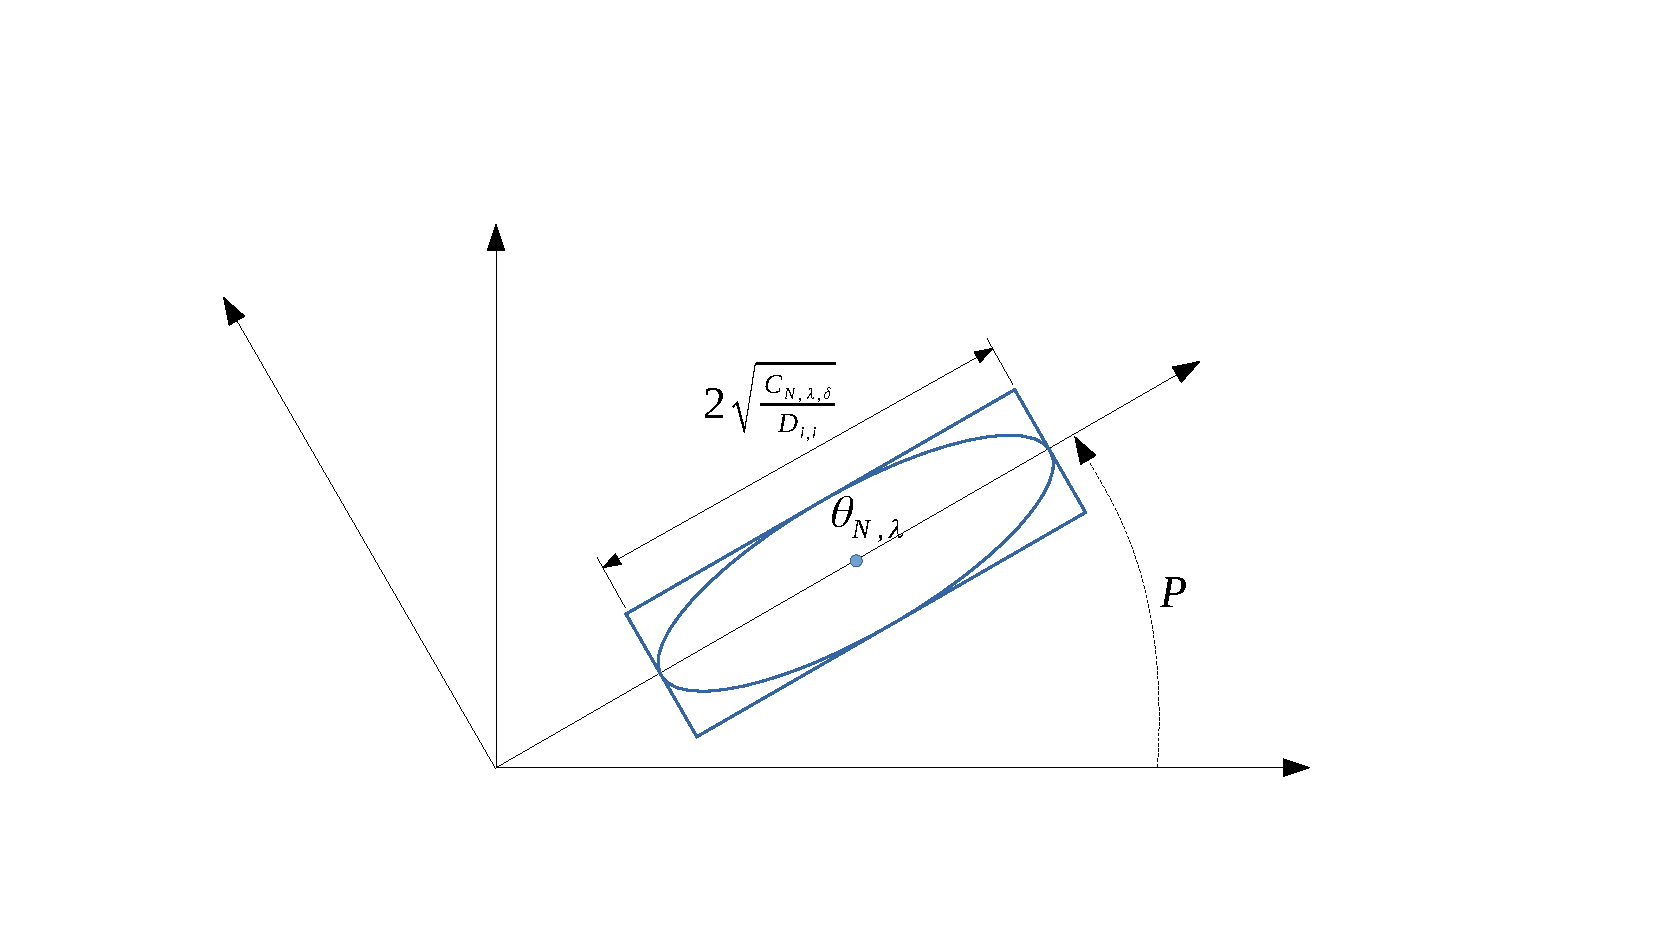
\includegraphics[trim={3.8cm, 2cm, 5cm, 3.8cm}, clip, width=0.7\linewidth]{img/ellipsoid_to_polytope}
		\caption{From the confidence ellipsoid $\cC_\confidence$ to its enclosing polytope $\cP_\confidence$}
		\label{fig:ellipsoid_to_polytope}
	\end{figure}
	
	\begin{lemma}[Confidence polytope]
		\label{lem:tight_polytope}
		\begin{leftbar}[lemmabar]
		We can enclose the confidence ellipsoid obtained in $\eqref{eq:confidence-ellipsoid}$ within a polytope
		\begin{equation}
		\cP = \left\{ A_{0}+\sum_{i=1}^{2^d}\lambda_{i}\Delta A_{i}: \lambda\in[0, 1]^{2^d},  \sum_{i=1}^{2^d}\lambda_{i}=1\right\}.
		\end{equation}
		with 
		\begin{align*}
		&h_k \text{ is the }k^\text{th}\text{ element of }\{-1,1\}^d\text{ for } k\in[2^d],\\
		&G_{N,\lambda} = PDP^{-1}, \quad \Delta\theta_k = \beta_{N}(\confidence)^{1/2} P^{-1}D^{-1/2} h_k, \\
		&A_0 = A + \theta_{N,\lambda}^\transp\phi, \quad \Delta A_k = \Delta\theta_k^\transp\phi.
		\end{align*}
		This conversion is illustrated in \Cref{fig:ellipsoid_to_polytope}.
		\end{leftbar}
	\end{lemma}

	\begin{proof}
		The ellipsoid in \eqref{eq:confidence-ellipsoid} is described by
		\begin{align*}
		\theta\in\confidenceset &\implies
		(\theta-\theta_{N,\lambda})^\transp G_{N,\lambda}(\theta-\theta_{N,\lambda}) \leq \beta_{N}(\confidence)\\
		&\implies (\theta'-\theta'_{N,\lambda})^\transp D (\theta'-\theta'_{N,\lambda}) \leq \beta_{N}(\confidence)\\
		&\implies \sum_{i=1}^d D_{i,i}(\theta'_i-\theta'_{N,\lambda,i})^2\leq \beta_{N}(\confidence)\\
		&\implies\forall i, |\theta'_i-\theta'_{N,\lambda,i}|\leq \beta_{N}(\confidence)^{1/2}D_{i,i}^{-1/2}
		\end{align*}
		This describes a $\Real^d$ box containing $\theta' = P\theta$, whose $k^\text{th}$ vertex is represented by $$\theta_{N,\lambda}' + \beta_{N}(\confidence)^{1/2}D^{-1/2} h_k.$$ We obtain the corresponding box on $\theta$ by transforming each vertex of the box with $P^{-1}$.
	\end{proof}

	
%		
%	\subsection{Experimental setting}
%	\label{sec:experimental-setting}
%	
%	In both experiments, we used $\discount=0.9$,  $\confidence=0.9$ and a planning budget $K=100$. The perturbations were sampled uniformly in $[-0.1, 0.1]^r$ while the measurements are Gaussian with covariance $\Sigma_r = 0.1 I_s$. 
%	
%	\subsection{Autonomous Driving}
%	
%	In the following, we describe the structure of the dynamical system $f$ representing the couplings and interactions between several vehicles.
%	
%	\paragraph{Kinematics}
%	
%	The kinematics of any vehicle $i\in[V]$ are represented by the Kinematic Bicycle Model:
%	\begin{align}
%	\dot{x}_i &= v_i\cos(\psi_i), \nonumber\\
%	\dot{y}_i &= v_i\sin(\psi_i), \nonumber\\
%	\dot{v}_i &= a_i, \nonumber\\
%	\dot{\psi}_i &= \frac{v_i}{l}tan(\beta_i), \nonumber
%	\end{align}
%	where $(x_i, y_i)$ is the vehicle position, $v_i$ is its forward velocity and $\psi_i$ is its heading, $l$ is the vehicle half-length, $a_i$ is the acceleration command and $\beta_i$ is the slip angle at the centre of gravity, used as a steering command.
%	
%	\paragraph{Longitudinal control}
%	Longitudinal behaviour is modelled by a linear controller using three features: a desired velocity, a braking term to drive slower than the front vehicle, and a braking term to respect a safe distance to the front vehicle.
%	
%	Denoting $f_i$ the index of the front vehicle preceding vehicle $i$, the acceleration command can be presented as follows:
%	\begin{equation*}
%	a_i = \begin{bmatrix}
%	\theta_{i,1} & \theta_{i,2} & \theta_{i,3}
%	\end{bmatrix} \begin{bmatrix}
%	v_0 - v_i \\
%	-(v_{f_i}-v_i)^- \\
%	-(x_{f_i} - x_i - (d_0 + v_iT))^- \\
%	\end{bmatrix},
%	\label{eq:theta_a}
%	\end{equation*}
%	where $v_0, d_0$ and $T$ respectively denote the speed limit, jam distance and time gap given by traffic rules.
%	
%	\paragraph{Lateral control}
%	
%	The lane $L_i$ with the lateral position $y_{L_i}$ and heading $\psi_{L_i}$ is tracked by a cascade controller of lateral position and heading $\beta_i$, which is selected in a way the closed-loop dynamics take the form
%	
%	\begin{align}
%	\label{eq:heading-command}
%	\dot{\psi}_i &= \theta_{i,5}\left(\psi_{L_i}+\sin^{-1}\left(\frac{\tilde{v}_{i,y}}{v_i}\right)-\psi_i\right),\\
%	\tilde{v}_{i,y} &= \theta_{i,4} (y_{L_i}-y_i). \nonumber
%	\end{align}
%	We assume that the drivers choose their steering command $\beta_i$ such that \eqref{eq:heading-command} is always achieved: $\beta_i = \tan^{-1}(\frac{l}{v_i}\dot{\psi}_i)$.
%	
%	\paragraph{LPV formulation}
%	
%	The system presented so far is non-linear and must be cast into the LPV form. We approximate the non-linearities induced by the trigonometric operators through equilibrium linearisation around $y_i=y_{L_i}$ and $\psi_i=\psi_{L_i}$.
%	
%	This yields the following longitudinal dynamics:
%	\begin{align*}
%	\dot{x}_i &= v_i,\\
%	\dot v_i &= \theta_{i,1} (v_0 - v_i) + \theta_{i,2} (v_{f_i} - v_i) + \theta_{i,3}(x_{f_i} - x_i - d_0 - v_i T),
%	\end{align*}
%	where $\theta_{i,2}$ and $\theta_{i,3}$ are set to $0$ whenever the corresponding features are not active.
%	
%	It can be rewritten in the form $$\dot{X} = \structureddynamics(X-X_c) + \omega.$$ For example, in the case of two vehicles only:
%	\begin{equation*}
%	X = \begin{bmatrix}
%	x_i \\
%	x_{f_i} \\
%	v_i \\
%	v_{f_i} \\
%	\end{bmatrix}
%	,\quad
%	X_c = \begin{bmatrix}
%	-d_0-v_0 T \\
%	0 \\
%	v_0\\
%	v_0 \\
%	\end{bmatrix}
%	,\quad
%	\omega = \begin{bmatrix}
%	v_0 \\
%	v_0 \\
%	0\\
%	0\\
%	\end{bmatrix}
%	\end{equation*}
%	
%	\begin{equation*}
%	\structureddynamics
%	=
%	\begin{blockarray}{ccccc}
%	& i & f_i & i & f_i \\
%	\begin{block}{c[cccc]}
%	i & 0 & 0 & 1 & 0 \\
%	f_i & 0 & 0 & 0 & 1 \\
%	i & -\theta_{i,3} & \theta_{i,3} & -\theta_{i,1}-\theta_{i,2}-\theta_{i,3} & \theta_{i,2} \\
%	f_i & 0 & 0 & 0 & -\theta_{f_i,1} \\
%	\end{block}
%	\end{blockarray}
%	\end{equation*}
%	
%	The lateral dynamics are in a similar form:
%	\begin{equation*}
%	\begin{bmatrix}
%	\dot{y}_i \\
%	\dot{\psi}_i \\
%	\end{bmatrix}
%	=
%	\begin{bmatrix}
%	0 & v_i \\
%	-\frac{\theta_{i,4} \theta_{i,5}}{v_i} & -\theta_{i,5}
%	\end{bmatrix}
%	\begin{bmatrix}
%	y_i - y_{L_i} \\
%	\psi_i - \psi_{L_i}
%	\end{bmatrix}
%	+
%	\begin{bmatrix}
%	v_i\psi_{L_i} \\
%	0
%	\end{bmatrix}
%	\end{equation*}
%	Here, the dependency in $v_i$ is seen as an uncertain parametric dependency, \ie $\theta_{i,6}=v_i$, with constant bounds assumed for $v_i$ using an overset of the longitudinal interval predictor.
%	
%	
%	\paragraph{Change of coordinates}
%	In both cases, the obtained polytope centre $A_0$ is non-Metzler.
%	We use the similarity transformation of coordinates of \citet{Efimov2013}. Precisely, we choose $\Theta$ such that for any $\theta\in\Theta$, $\structureddynamics$ is always diagonalisable with real eigenvalues, and perform an eigendecomposition to compute its change of basis matrix $Z$. The transformed system $X'=Z^{-1}(X-X_c)$ verifies \eqref{eq:confidence} with $A_0$ Metlzer as required to apply the interval predictor of \Cref{prop:predictor}. Finally, the obtained predictor is transformed back to the original coordinates $Z$ by using the following lemma:
%	\begin{lemma}[Interval arithmetic of \citealp{Efimov2012}]
%		\label{lem:interval} Let $x\in\mathbb{R}^{n}$ be a vector variable, $\underline{x}\le x\le\overline{x}$ for some $\underline{x},\overline{x}\in\mathbb{R}^{n}$. 
%		
%		\begin{enumerate}
%			\item If $A\in\Real^{m\times n}$ is a constant matrix, then
%			\begin{equation}
%			A^{+}\underline{x}-A^{-}\overline{x}\le Ax\le A^{+}\overline{x}-A^{-}\underline{x}.\label{eq:Interval1}
%			\end{equation}
%			\item If $A\in\Real^{m\times n}$ is a matrix variable and \textup{$\underline{A}\le A\le\overline{A}$} for some $\underline{A},\overline{A}\in\Real^{m\times n}$, then
%			\begin{gather}
%			\underline{A}^{+}\underline{x}^{+}-\overline{A}^{+}\underline{x}^{-}-\underline{A}^{-}\overline{x}^{+}+\overline{A}^{-}\overline{x}^{-}\leq Ax\label{eq:Interval2}\\
%			\leq\overline{A}^{+}\overline{x}^{+}-\underline{A}^{+}\overline{x}^{-}-\overline{A}^{-}\underline{x}^{+}+\underline{A}^{-}\underline{x}^{-}.\nonumber 
%			\end{gather}
%		\end{enumerate}
%	\end{lemma}
	
%	\paragraph{Actions}
%	
%	The action space $\cA$ is constituted of five actions: faster, slower, lane change to the right, lane change to the left, and no-op. They are implemented by a lateral linear controller that track a reference lateral position $y_L$, affected by the lane change actions, and a lateral longitudinal linear controller that tracks the desired velocity $v_0$, affected by the faster and slower actions.
%	
%	\paragraph{Reward}
%	
%	The reward function $R$ is the following:
%	\[
%	R(x) = 
%	\begin{cases}
%	1 & \text{if the ego-vehicle is at full velocity;}\\
%	0 & \text{if the ego-vehicle has collided with another vehicle;}\\
%	0.5 & \text{else.}
%	\end{cases}\]
	

\end{appendices}

	\newpage

%	\begin{small}   % XXX

	% %!TEX root = ../PhD_thesis__Edouard_Leurent
% ******************************* Thesis Appendix A ****************************
\chapter*{List of Publications}
\addcontentsline{toc}{chapter}{List of Publications}

\section*{International Workshops}
\renewcommand{\labelenumi}{[IW-\arabic{enumi}]}
\begin{etaremune}
\end{etaremune}

\section*{International Conferences}
\renewcommand{\labelenumi}{[IC-\arabic{enumi}]}
\begin{etaremune}
\end{etaremune}

	% **************** Listes *****************
%	\begin{spacing}{1.00}%
	{% group, to change the \cleardoublepage
		% FIXME force to not have a blank (even numbered) page between lists
		% https://tex.stackexchange.com/questions/69184/remove-blank-page-between-list-of-figures-and-list-of-tables#69218
		\let\cleardoublepage\clearpage%
		\listoffigures
		\mtcaddchapter
		\let\cleardoublepage\clearpage%
		\listofalgorithms
		\mtcaddchapter[List of Algorithms]
		\let\cleardoublepage\clearpage%
		\listoftables
		\mtcaddchapter
	}
%	\end{spacing}

	% *************** Bibliography ****************
	\begin{spacing}{0.93}
%		\bibliographystyle{apalike}
%		\bibliographystyle{apacite}
%		\bibliographystyle{alpha}
%		\bibliographystyle{plainnat}
		\cleardoublepage
		% \nocite{*}
%		\bibliography{all-phd-thesis,chapter4,chapter5,chapter6,chapter7,chapter7_2,contributions}

		\printbibliography[heading=bibintoc]
		\adjustmtc

%		\vfill{}
%		\hr{}		
%		\begin{small}
%			\begin{quote}
%				\emph{Visite aussi beaucoup de villes égyptiennes,}\\
%				\emph{et n’aie de cesse de t’instruire auprès de ceux qui savent.}\\
%				Konstantinos Kavafis, \emph{Ithaki}.
%			\end{quote}
%		\end{small}
	\end{spacing}

%	\end{small}

	\backmatter
	\cleartoleftpage
	% \begin{backpage} %backpage
% \setsinglecolumn
% \vspace*{0.2\textheight}
\thispagestyle{empty}
\pagestyle{plain}
%\includepdf[pages={1}]{6-Back/Back.pdf}
% \end{backpage}

\end{document}
